%%%%%%%% ICML 2024 EXAMPLE LATEX SUBMISSION FILE %%%%%%%%%%%%%%%%%

\documentclass{article}

% Recommended, but optional, packages for figures and better typesetting:
\usepackage{microtype}
\usepackage{graphicx}
\usepackage{booktabs} % for professional tables
\usepackage{pgfplots}
\usepackage{pgfplotstable}
\usepackage{hyperref}
\usepackage{tabularray}


% hyperref makes hyperlinks in the resulting PDF.
% If your build breaks (sometimes temporarily if a hyperlink spans a page)
% please comment out the following usepackage line and replace
% \usepackage{icml2024} with \usepackage[nohyperref]{icml2024} above.
\usepackage{hyperref}


% Attempt to make hyperref and algorithmic work together better:
\newcommand{\theHalgorithm}{\arabic{algorithm}}

% Use the following line for the initial blind version submitted for review:
% \usepackage{icml2024}

% If accepted, instead use the following line for the camera-ready submission:
\usepackage[accepted]{icml2024}

% For theorems and such
\usepackage{amsmath}
\usepackage{amssymb}
\usepackage{mathtools}
\usepackage{amsthm}
\usepackage{xspace}
\usepackage{multirow}
\usepackage{tcolorbox}
\usepackage{adjustbox}
\usepackage{makecell}
\usepackage{subfig}
% if you use cleveref..
\usepackage[capitalize,noabbrev]{cleveref}

\usepackage{balance}

\captionsetup[subfloat]{labelformat=simple, labelsep=colon}
\renewcommand{\thesubfigure}{\thefigure.\arabic{subfigure}}

%%%%%%%%%%%%%%%%%%%%%%%%%%%%%%%%
% THEOREMS
%%%%%%%%%%%%%%%%%%%%%%%%%%%%%%%%
\theoremstyle{plain}
\newtheorem{theorem}{Theorem}[section]
\newtheorem{proposition}[theorem]{Proposition}
\newtheorem{lemma}[theorem]{Lemma}
\newtheorem{corollary}[theorem]{Corollary}
\theoremstyle{definition}
\newtheorem{definition}[theorem]{Definition}
\newtheorem{assumption}[theorem]{Assumption}
\theoremstyle{remark}
\newtheorem{remark}[theorem]{Remark}
\pgfplotsset{compat=1.17}

% Todonotes is useful during development; simply uncomment the next line
%    and comment out the line below the next line to turn off comments
%\usepackage[disable,textsize=tiny]{todonotes}
\usepackage[textsize=tiny]{todonotes}
% The \icmltitle you define below is probably too long as a header.
% Therefore, a short form for the running title is supplied here:

\newcommand{\q}[1]{``{#1}''}
\newcommand{\tool}{Deep-Bench\xspace}
\newcommand*\circled[1]{\tikz[baseline=(char.base)]{
            \node[shape=circle,draw,inner sep=2pt] (char) {#1};}}

\icmltitlerunning{\tool: Deep Learning Benchmark Dataset for Code Generation}

\begin{document}

\newcommand{\thought}[1]{{\color[rgb]{0.2,0.39,0.66}(#1)}}
\newcommand{\todo}[1]{{\color[rgb]{1.0,0.0,0.0}(#1)}}
\newcommand{\hsh}[1]{{\color{green!50!black} Henrik: #1}}
\newcommand{\st}[1]{{\color{red!50!black} Sebastian: #1}}

\newcommand{\ulm}[1]{_{\scaleto{\mathrm{#1}}{3pt}}}
\newcommand\at[2]{\left.#1\right|_{#2}}











\newtheorem{assumption}{Assumption}

\DeclareMathOperator*{\argmax}{arg\,max}
\DeclareMathOperator*{\argmin}{arg\,min}

\newcommand{\swname}[1]{\texttt{#1}}
\newcommand{\ie}{i\/.\/e\/.,\/~}
\newcommand{\eg}{e\/.\/g\/.,\/~}
\newcommand{\cf}{cf\/.\/~}

\newcommand{\fig}{Fig\/.\/~}
\newcommand{\defn}{Def\/.\/~}
\newcommand{\sect}{Sec\/.\/~}
\newcommand{\tabl}{Tab\/.\/~}
\newcommand{\algo}{Algorithm~}
\newcommand{\theo}{Theorem~}

\newcommand{\bnnl}{3 hidden layers}
\newcommand{\bnnn}{50 neurons}
\newcommand{\bnna}{tanh activations}

\newcommand{\capt}[1]{\mdseries{\emph{#1}}}

\newcommand{\videolink}{at \url{https://youtu.be/_d7AqTRjz6g}}
\newcommand{\codelink}{\url{https://github.com/wheelbot/mini-wheelbot}}

\newcommand{\fakepar}[1]{\vspace{0mm}\noindent\textbf{#1.}}

\newcommand{\needref}{\textcolor{red}{[REF]}}

\newcommand{\plotfontsize}{9pt}


\twocolumn[
    \icmltitle{\tool: Deep Learning Benchmark Dataset for Code Generation}

    % You may provide any keywords that you
    % find helpful for describing your paper; these are used to populate
    % the "keywords" metadata in the PDF but will not be shown in the document
    % It is OKAY to include author information, even for blind
% submissions: the style file will automatically remove it for you
% unless you've provided the [accepted] option to the icml2024
% package.

% List of affiliations: The first argument should be a (short)
% identifier you will use later to specify author affiliations
% Academic affiliations should list Department, University, City, Region, Country
% Industry affiliations should list Company, City, Region, Country

% You can specify symbols, otherwise they are numbered in order.
% Ideally, you should not use this facility. Affiliations will be numbered
% in order of appearance and this is the preferred way.
\icmlsetsymbol{equal}{*}

\begin{icmlauthorlist}
\icmlauthor{Alireza Daghighfarsoodeh}{yyy}
\icmlauthor{Chung-Yu Wang}{yyy}
\icmlauthor{Hamed Taherkhani}{yyy}
\icmlauthor{Melika Sepidband}{yyy}
\icmlauthor{Mohammad Abdollahi}{yyy}
\icmlauthor{Hadi Hemmati}{yyy}
\icmlauthor{Hung Viet Pham}{yyy}
%\icmlauthor{}{sch}
%\icmlauthor{}{sch}
%\icmlauthor{}{sch}
\end{icmlauthorlist}

\icmlaffiliation{yyy}{Department of EECS, York University, Toronto, Canada}

    \icmlkeywords{Benchmark, Large Language Model, ICML}
    
\vskip 0.3in
]



\begin{abstract}
\begin{abstract}

% Recent works to jointly reconstruct 3D human and object from a single RGB image, are mostly model-based, that fail to capture the fine details of the clothed human body and object surface. In this paper, we introduce ReCHOR, a novel, model-free, first-method to produce realistic clothed human-object reconstructions from a monocular view. This is extremely challenging due to human-object occlusions, diverse interactions and depth ambiguity, as it needs to infer both 3D spatial awareness and high resolution details. Our core idea is based on estimating neural implicit representations for human and object respectively by an attention-based neural implicit model that attends to pixel-aligned features from both the global human-object image for spatial awareness and  the local separate view of human and object images for high quality details. Additionally, the network is conditioned on semantic features from an initial estimated human-object pose prior and a generative diffusion model that inpaints occluded regions, thus enabling the retrieval of details from them.
% We also propose a synthetic dataset with rendered scenes of diverse, inter-occluded 3D human and object scans, to train our network. We evaluate our method on the synthetic and real world BEHAVE dataset. Our experiments show that our method outperforms the SOTA in achieving realistic clothed human-object reconstructions.
Recent approaches to jointly reconstruct 3D humans and objects from a single RGB image represent 3D shapes with template-based or coarse models, which fail to capture details of loose clothing on human bodies. In this paper, we introduce a novel implicit approach for jointly reconstructing realistic 3D clothed humans and objects from a monocular view. For the first time, we model both the human and the object with an implicit representation, allowing to capture more realistic details such as clothing. This task is extremely challenging due to human-object occlusions and the lack of 3D information in 2D images, often leading to poor detail reconstruction and depth ambiguity. To address these problems, we propose a novel attention-based neural implicit model that leverages image pixel alignment from both the input human-object image for a global understanding of the human-object scene and from local separate views of the human and object images to improve realism with, for example, clothing details. Additionally, the network is conditioned on semantic features derived from an estimated human-object pose prior, which provides 3D spatial information about the shared space of humans and objects. To handle human occlusion caused by objects, we use a generative diffusion model that inpaints the occluded regions, recovering otherwise lost details. For training and evaluation, we introduce a synthetic dataset featuring rendered scenes of inter-occluded 3D human scans and diverse objects. Extensive evaluation on both synthetic and real-world datasets demonstrates the superior quality of the proposed human-object reconstructions over competitive methods.
\end{abstract}
\end{abstract}

\section{Introduction}
\label{sec:intro}
% Image editing methods in diffusion models depend on user-defined control directions - users can unlock their creativity using these methods by specifying the desired manipulation through prompts~\cite{gandikota2023concept}, reference images~\cite{ruiz2022dreambooth, kumari2022customdiffusion, gal2022image, chen2024trainingfreeregionalpromptingdiffusion}, or attribute vectors~\cite{parmar2023zero,hertz2022prompt}. In this work, we ask a fundamentally different question: \emph{Can we automatically discover the underlying visual structure of a concept within diffusion model's knowledge?} %Rather than requiring user-specified controls, we aim to decompose the model's internal knowledge into meaningful directions.

% This question touches on a fundamental limitation in how we interact with diffusion models. Current control methods ~\cite{zhang2023addingconditionalcontroltexttoimage, gandikota2023concept, ye2023ipadaptertextcompatibleimage,ye2023ipadaptertextcompatibleimage, hertz2024stylealignedimagegeneration, li2023photomaker, shi2024instantbooth, chen2024trainingfreeregionalpromptingdiffusion} require users to specify their desired manipulations in advance, limiting interactive creativity. This contrasts with natural human artistic workflows, where creators dynamically explore creative ideas while jointly refining them toward meaningful artistic outcomes~\cite{hoffmann2016modeling}. This synergy between specification and exploration is not new to generative models. Early GAN architectures naturally developed disentangled latent spaces that enabled continuous\cite{harkonen2020ganspace,radford2015unsupervised, wu2021stylespace, shen2020interfacegan}, compositional control over generated images. Users could explore these spaces to discover interesting variations that would be difficult to describe in words~\cite{wu2021stylespace}, then combine them to achieve their creative goals~\cite{grabe2022towards}. 


% While diffusion models have largely superseded GANs in conditional image synthesis~\cite{dhariwal2021diffusion},  their underlying structure remains less understood. Diffusion models achieve remarkable diversity through high-dimensional latents, unlike GANs' compact latent spaces.  With a single prompt, diffusion models can generate radically different variations through different random initializations of input noise. We ask - Is it possible to discover interpretable structure within this vast space of variations?

Text-to-image diffusion models are capable of generating remarkable visual variations from a single prompt through different random initializations. However, this vast creative potential remains largely opaque to users---while we can generate diverse images, we lack understanding of the underlying structure of these variations. This presents a fundamental challenge: how can we discover and expose the latent visual capabilities encoded within these models?

\let\thefootnote\relax \footnote{$^{*}$Correspondence to \texttt{gandikota.ro@northeastern.edu}}

The challenge touches on a key limitation in how we interact with diffusion models today. Current control methods require users to explicitly specify their desired edits in advance through prompts~\cite{gandikota2023concept}, reference images~\cite{zhang2023addingconditionalcontroltexttoimage, chen2024trainingfreeregionalpromptingdiffusion, ruiz2022dreambooth,kumari2022customdiffusion, Ryu_lora, hu2021lora}, or attribute vectors~\cite{ye2023ipadaptertextcompatibleimage, hertz2024stylealignedimagegeneration, li2023photomaker, shi2024instantbooth,parmar2023zero,hertz2022prompt}. That contrasts sharply with natural human creative workflows, where artists dynamically explore creative ideas and jointly refine them toward meaningful artistic outcomes~\cite{hoffmann2016modeling}. The need for pre-specified controls creates a barrier between users and the full creative potential of these models.

Interestingly, earlier generative models like GANs~\cite{gans,karras2019style,brock2018large} naturally developed more interpretable internal structures. Their compact latent spaces often exhibited emergent disentanglement~\cite{harkonen2020ganspace,radford2015unsupervised, wu2021stylespace, shen2020interfacegan}, enabling continuous and compositional control over generated images. Users could explore these spaces to discover interesting variations that would be difficult to describe in words~\cite{wu2021stylespace}, then combine them to achieve their creative goals~\cite{grabe2022towards}.

Diffusion models have largely superseded GANs in conditional image synthesis~\cite{dhariwal2021diffusion}, achieving greater diversity through much higher-dimensional latents. And yet an understanding of the underlying structure of these larger latent spaces has remained elusive. In this work, we ask a fundamental question: \emph{Can we automatically discover the visual structure within a diffusion model's knowledge of a concept?} Rather than requiring user-specified controls, we aim to decompose the model's internal representations into expressive directions that users can explore and combine.

To address these needs, we present \textbf{SliderSpace}, a framework that brings systematic explorability to diffusion models. Given just a text prompt, SliderSpace discovers a canonical set of meaningful, diverse, and controllable directions within the model's knowledge of that concept. Each direction is implemented as a low-rank adapter~\cite{hu2021lora} that can be scaled and composed with others, allowing users to explore and smoothly combine different aspects of variation, as shown in Figure~\ref{fig:intro}.

We ground SliderSpace discovery in three key requirements for meaningful decomposition of a diffusion model's visual manifold: 
\begin{enumerate}
    \item \textbf{Unsupervised Discovery:} The decomposition process should emerge from the intrinsic structure of the model's learned representation, rather than being guided by predefined attributes. This ensures we capture the true topology of the model's knowledge space rather than projecting our assumptions onto it.
    
    \item \textbf{Semantic Orthogonality:} Each discovered control must represent a distinct semantic direction. This is enforced in a semantic feature space, like CLIP, where every slider has an orthogonal effect in embeddings. This prevents discovering multiple controls that create similar semantic effects, making the system more efficient and easier.
    
    \item \textbf{Distribution Consistency:} Directions must induce consistent transformations across both random seeds and prompt variations. 
\end{enumerate}

These requirements naturally lead to our proposed framework, which we formalize in Section~\ref{sec:method}. As we show in our experiments, SliderSpace is architecture-agnostic, working with both conventional U-Net based models like Stable Diffusion~\cite{rombach2022high, rombach2022sd20, podell2023sdxl, turbo, dmd} and recent transformer-based architectures like Flux~\cite{flux}.

We demonstrate the expressiveness of SliderSpace through three applications: First, we show how SliderSpace can decompose high-level concepts into diverse and expressive components, revealing the natural axes of variation in the model's understanding. Second, we explore artistic style variation, where SliderSpace discovers directions that match or exceed the diversity of manually curated artist lists while being judged more useful by human evaluators. Finally, we show how SliderSpace can help reverse the mode collapse commonly observed in distilled diffusion models, restoring diversity while maintaining generation speed.

Beyond providing practical creative control, SliderSpace opens new avenues for understanding and utilizing the latent capabilities of diffusion models. By mapping these models' visual potential into intuitive, composable directions, we take a step toward making their creative possibilities more accessible and interpretable to users.

% Image editing methods in diffusion models unlock the creativity of users. In this work we ask an alternate question: \emph{Can we organize and expose what of the diffusion model is already capable of?}.
% Existing methods for controlling image generation typically require users to manually specify edit directions for desired changes. This process is time-consuming, requires technical expertise, and limits the spontaneity of the creative process. For instance, if a user wants to adjust the smile of a generated person, they must explicitly request this edit, often through imprecise prompt engineering or model fine-tuning. This approach of predefined controls or manual specifications restricts users from fully exploring the latent capabilities of the model. There may be interesting stylistic variations or attributes that the model can generate, but users have no easy way to discover or utilize these.

% Natural visual disentanglement was an emergent property in the latent space of Generative Adversarial Models (GANs) \cite{harkonen2020ganspace,radford2015unsupervised, wu2021stylespace, shen2020interfacegan}. In particular, it has been observed that StyleGAN~\cite{karras2019style} stylespace neurons offer detailed control over many meaningful aspects of images that would be difficult to describe in words~\cite{wu2021stylespace}. However, diffusion models do not share such a compact latent space~\cite{park2023unsupervised}; and efforts to uncover such a space in the semantic embeddings of the text conditioning have met with limited success \nik{Nick - is there a specific citation you were thinking about?}.

% In this work we introduce \textbf{SliderSpace}, which takes a step towards uncovering an analogous low dimensional representation of diffusion models' visual breadth; in essence treating the diffusion model as many generators sharing parameters, where a particular generator is defined by a specific prompt. For a given prompt we sample many random seeds (and optionally prompt expansions using an LLM), generate the corresponding images, and apply an off the shelf feature extractor (in this work CLIP, but our method can be applied to any differentiable feature extractor). We use PCA to analyze these features, and for each of the leading $k$ principal components we train a LoRA \cite{} which causes the diffusion model to produces images which increase the feature magnitude along that component when passed back through the same feature extractor. This leads to a 'Slider' for each principal component, because each LoRA can be scaled and applied to the original diffusion model, continuously varying those visual features in the generated results (as measured, in our case, by CLIP).

% There are many other works that enhance the controllability of diffusion models. One common approach is enabling users to add spatial constraints to a generation either manually, or via a reference image \cite{zhang2023addingconditionalcontroltexttoimage, chen2024trainingfreeregionalpromptingdiffusion}, a second is leveraging more abstract embeddings (e.g. identity, style) extracted from a reference image \cite{ye2023ipadaptertextcompatibleimage, hertz2024stylealignedimagegeneration, li2023photomaker, shi2024instantbooth}, a third is finetuning a foundation model to better generate a concept important to the user \cite{ruiz2022dreambooth, kumari2022customdiffusion, Ryu_lora, hu2021lora}, and a fourth (most relevant to this work) is finding low-rank adaptors of the model based on a prompt or small training set which can be scaled to provide continous control over one aspect of generated image (e.g. night vs day, basic vs luxury, etc.) \cite{gandikota2023concept}. SliderSpace is complementary to all of these methods and offers something distinct. All of the other methods we are aware require the user (and / or model designer) to know in advance what type of control they want. In contrast SliderSpace assists users in discovering and controlling hidden capabilities present in the diffusion model's distribution of possible generations.

%We propose that truly intuitive creative control in a text-to-image model should meet three key criteria: \emph{discoverability}, \emph{intuitiveness}, and \emph{specificity}. The model should reveal controllable attributes that may not be immediately obvious, offer controls that are easy to understand and manipulate, and ensure each control affects a distinct attribute of the generated image.

% We demonstrate the utility and power of SliderSpace using three applications built on top of SDXL-DMD \cite{dmd}, because its fast generation speed lends itself well to the continuous control offered by SliderSpace.

% First, we study concept decomposition (Section \ref{sec:concept_exp}), where we learn sliders for a specific concept (e.g. 'monster', 'waterfall', 'car'). Through quantitative metrics of diversity and text alignment we demonstrate that the learned sliders dramatically boost the diversity of generations when randomly applied without harming text alignment; we also ask humans to qualitatively judge these results in a user study where they find the SliderSpace results to be more 'Diverse', 'Useful', and 'Creative' than our baselines.

% Second, we attempt to compare the automatic discoveries of SliderSpace to a large scale manual study of artistic styles (Section \ref{sec:art_exp}), open-sourced by ParrotZone \cite{parrotzone}. In this study SDXL was prompted with over 4300 artist names,  and based on visual inspection the cases of successful stylistic mimicry recorded. Quantitatively SliderSpace more closely matches the distribution of artistic variation discovered by ParrotZone than other baselines, and in our user studies was judged to be significantly more 'Diverse' and 'Useful' than the baselines. To our surprise humans even judged SliderSpace results to be slightly more 'Diverse' than the results generated by the manually discovered artist names of \cite{parrotzone}.

% Third, we attempt to use SliderSpace to reverse the mode collapse commonly observed in distilled few-step diffusion models relative to the original teacher model (Section \ref{sec:diverse_exp}). We quantitatively demonstrate that applying SliderSpace to SDXL-DMD leads to more closely matching the distribution of images by the original teacher, SDXL.

%Through extensive experiments on various state-of-the-art text-to-image models, we demonstrate that SliderSpace significantly enhances user control and creative expression in AI-assisted image generation tasks. Our method enables a range of applications, including concept decomposition and control, diversity improvement in generated images, customization dissection and edits, and the exploration of artistic styles inherent in the model.

% SliderSpace goes beyond providing a practical tool for enhanced creative control. By mapping the visual potential of diffusion models it can open new avenues for generative creativity and deepens our understanding of each model's hidden potential.
\section{Related Work}

\paragraph{LLMs for Agent tasks.}

Our research is related to deploying large language models (LLMs) as agents for decision-making tasks in interactive environments~\citep{liu2023agentbench,zhou2023webarena,shridhar2020alfred,toyama2021androidenv}. Earlier works, such as~\citep{yao2023webshopscalablerealworldweb}, fine-tuned models like BERT~\citep{devlin2019bertpretrainingdeepbidirectional} for decision-making in simplified environments, such as online shopping or mobile phone manipulation. With the advent of large language models~\citep{brown2020languagemodelsfewshotlearners,openai2024gpt4technicalreport}, it became feasible to perform decision-making tasks through zero-shot or few-shot in-context learning. To better assess the capabilities of LLMs as agents, several models have been developed~\citep{deng2024mind2web,xiong2024watch,hong2023cogagent,yan2023gpt}. Most approaches~\citep{zheng2024seeact,deng2024mind2web} provide the agent with observation and action history, and the language model predicts the next action via in-context learning. Additionally, some methods~\citep{zhang2023building,li2023camel,song2024trial} attempt to distill trajectories from state-of-the-art language models to train more effective policy models. In contrast, our paper introduces a novel framework that automatically learns a reward model from LLM agent navigation, using it to guide the agents in making more effective plans.

\textbf{LLM Planning.} Our paper is also related to planning with large language models. Early researchers~\citep{brown2020languagemodelsfewshotlearners} often prompted large language models to directly perform agent tasks. Later, \citet{yao2022react} proposed ReAct, which combined LLMs for action prediction with chain-of-thought prompting~\citep{wei2022chain}. Several other works~\citep{yao2023treethoughtsdeliberateproblem,hao2023reasoning,zhao2023large,qiao2024agentplanningworldknowledge} have focused on enhancing multi-step reasoning capabilities by integrating LLMs with tree search methods. Our model differs from these previous studies in several significant ways. First, rather than solely focusing on text generation tasks, our pipeline addresses multi-step action planning tasks in interactive environments, where we must consider not only historical input but also multimodal feedback from the environment. Additionally, our pipeline involves automatic learning of the reward model from the environment without relying on human-annotated data, whereas previous works rely on prompting-based frameworks that require large commercial LLMs like GPT-4~\citep{openai2024gpt4technicalreport} to learn action prediction. Furthermore, \Model supports a variety of planning algorithms beyond tree search.

\textbf{Learning from AI Feedback.} In contrast to prior work on LLM planning, our approach also draws on recent advances in learning from AI feedback~\citep{bai2022constitutional,lee2023rlaif,yuan2024self,sharma2024critical,pan2024autonomous,koh2024tree}. These studies initially prompt state-of-the-art large language models to generate text responses that adhere to predefined principles and then potentially fine-tune the LLMs with reinforcement learning. Like previous studies, we also prompt large language models to generate synthetic data. However, unlike them, we focus not on fine-tuning a better generative model but on developing a classification model that evaluates how well action trajectories fulfill the intended instructions. This approach is simpler, requires no reliance on state-of-the-art LLMs, and is more efficient. We also demonstrate that our learned reward model can integrate with various LLMs and planning algorithms, consistently improving their performance.

\textbf{Inference-Time Scaling.} ~\citet{snell2024scaling} validates the efficacy of inference-time scaling for language models. Based on inference-time scaling, various methods have been proposed, such as random sampling~\citep{wang2022self} and tree-search methods~\citep{hao2023reasoning, zhang2024accessing, guan2025rstar}. Concurrently, several works have also leveraged inference-time scaling to improve the performance of agentic tasks. ~\citet{koh2024tree} adopts a training-free approach, employing MCTS to enhance policy model performance during inference and prompting the LLM to return the reward. ~\citet{gu2024your} introduces a novel speculative reasoning approach to bypass irreversible actions by leveraging LLMs or VLMs. It also employs tree search to improve performance and prompts an LLM to output rewards. ~\citet{yu2024exact} proposes Reflective-MCTS to perform tree search and fine-tune the GPT model, leading to improvements in ~\citet{koh2024visualwebarena}. ~\citet{putta2024agent} also utilizes MCTS to enhance performance on web-based tasks such as ~\citet{yao2023webshopscalablerealworldweb} and real-world booking environments. ~\cite{lin2025qlass} utilizes the stepwise reward to give effective intermediate guidance across different agentic tasks. Our work differs from previous efforts in two key aspects: (1) Broader Application Domain. Unlike prior studies that primarily focus on tasks from a single domain, our method demonstrates strong generalizability across web agents, mathematical reasoning, and scientific discovery domains, further proving its effectiveness. (2) Flexible and Effective Reward Modeling. Instead of simply prompting an LLM as a reward model, we finetune a small scale VLM~\citep{lin2023vila} to evaluate input trajectories. %Our reward scores range continuously between 0 and 1, in contrast to existing methods that rely on discrete scoring (e.g., 0 and 1, or 0, 0.5, and 1) through direct LLM prompting.

% Concurrently, several works have also leveraged inference-time scaling to improve the performance of agentic tasks. ~\citet{pan2024autonomous} demonstrates that LLMs and VLMs, such as the GPT series, can function as evaluators or reward models to provide guidance for fine-tuning or reflection, thereby enhancing digital agents. This lays the groundwork for subsequent studies that directly prompt LLMs as reward models. ~\citet{koh2024tree} adopts a training-free approach, employing MCTS to enhance policy model performance during inference. However, it is limited to web environments~\citep{koh2024visualwebarena}. Moreover, its value function relies on prompting an LLM, which is less effective than our proposed method. We validate our approach through ablation studies, demonstrating that our fine-tuned reward model is more effective. ~\citet{gu2024your} introduces a novel speculative reasoning approach to bypass irreversible actions, such as purchasing a product, by leveraging LLMs or VLMs. It also employs tree search to improve performance, but it remains restricted to the web domain~\citep{koh2024visualwebarena, deng2024mind2web}. Additionally, it lacks reward modeling and instead prompts an LLM to output rewards. ~\citet{yu2024exact} proposes Reflective-MCTS to perform tree search and fine-tune the GPT model, leading to improvements in ~\citep{koh2024visualwebarena}. However, this work focuses solely on a single web agent task, and its reward modeling is derived from multi-agent debate, differing from our more effective and efficient reward modeling approach. ~\citet{putta2024agent} also utilizes MCTS to enhance performance, but it is limited to web-based tasks such as ~\citep{yao2023webshopscalablerealworldweb} and real-world booking environments.
\section{Benchmark Construction}
\label{sec:BenchConstr}

\begin{figure*}[h!]
    \centering
    \includegraphics[width=\linewidth]{figs/pipeline_v2.pdf}
    \vspace{-40mm}
    \caption{Overview of our two-stage training pipeline {\ours}.}
    \label{fig:pipeline}
\end{figure*}

\begin{figure}
    \centering
    \includegraphics[width=\linewidth]{figs/last_template.pdf}
    %\vspace{-7pt}
    \caption{Template of generating prompt from code}
    
    \label{fig:code_prompt}
    \vspace{-10pt}
    
\end{figure}
%\subsection{Overview}

\tool consists of 520 instances of AI and DL data points (filtered from over 2,000 raw data points). The data is curated from 30 GitHub repositories (selected from an initial pool of 160 related repositories).

%In this section, we will discuss the step-by-step process of constructing \tool as demonstrated in Figure~\ref{fig:pipeline}. 
The construction process of \tool consists of two main phases: The Raw Data Extraction and the Labeling Procedure. The raw data extraction involves six semi-automatic steps. Since \tool is designed to have diverse and realistic code samples, the first step \circled{1} is to construct \tool from code crawled from highly rated GitHub repositories (i.e., with the most stars) filtered using 30 DL-related terms such as ``neural-networks'',  ``pytorch'', ``computer-vision''. We then manually select (step \circled{2}) 160 high quality candidate DL projects 
%that are considered DL related 
%to make DL benchmark in code generation, as they 
(i.e., involve the integration of DL and AI-related frameworks, comprehensive test cases, clear and well-written docstrings, and detailed contribution guidelines). We then employed a bespoke utility to extract the test files and then test cases from each repository (step \circled{3} and \circled{4}). By performing static analysis, we were able to track and collect all of the functions under test in step \circled{5} to form the raw data that is the base of \tool. 

Once the raw data is extracted, the labeling procedure starts. To speed up the task of constructing the prompt for each code sample, we utilize LLM (i.e., GPT-4o) as a code-explanation tool\cite{nam2024using} to generate the first prompt candidate for each function under test (step \circled{7}). Four co-authors were then tasked with manually filtering each entry to ensure that each function is highly relevant (i.e., contributes to a DL task such as image recognition, utilizes at least one recognized DL framework, and implements a relatively advanced and sophisticated algorithm).
Finally, we conduct a manual labeling process involving four co-authors (step \circled{9}) to refine the prompt and label each code sample with the appropriate category from our three chosen types of categories: DL pipeline phases, ML task types, and input types.


% (melika) It's better to explain how you generate the prompts. You just mentioned that they are generated automatically.
%In summary, the steps needed for building \tool is as follows:
%\begin{enumerate}
%    \item We gathered 30 different GitHub tags related to deep learning, like ``neural-networks'' (details in Section~\ref{sec:rs}).
%    \item We crawled GitHub and extracted related repositories with those tags, filtering for those that were more recently updated and had more than 400 stars (details in Section~\ref{sec:rs}).
%    \item We manually cherry-picked 160 repositories for more detailed data extraction and cloned them (details in Section~\ref{sec:rs}).
%    \item We extracted test cases within each repository (details in Section~\ref{sec:fe}).
%    \item We then extracted functions that are called in the test suites, ensuring they were not third-party functions (details in Section~\ref{sec:fe}).
%    \item We crawled each repository to extract the function definitions, forming the first version of our raw data (details in Section~\ref{sec:fe}).
%    \item We used code-explanation tools, such as LLMs, to generate prompts based on the function definitions (details in Section~\ref{sec:pg}).
%    \item We manually checked each function definition and rated them for relevance to deep learning, involving 2-3 people in the review process (details in Section~\ref{sec:rd}).
%    \item Finally, we manually checked and modified each prompt, integrating the generated prompts with doc-strings within each function to ensure clarity and accuracy (details in Section~\ref{sec:lp}).
%\end{enumerate}
%These steps are demonstrated in Fig.~\ref{fig:pipeline}. In the following sections, we will provide a more detailed explanation of each step.

\subsection{Raw Data Extraction}

This phase consists of six semi-automatic steps that crawl data from GitHub repositories to generate a list of function definitions and their test cases.

%\subsubsection{}
%\label{sec:rs}

%One of the characteristics of \tool is the source of its origin. 
%Unlike other datasets, which may draw from limited or outdated sources, 
%We curated our data from the most starred DL-related GitHub repositories
%~\cite{shrivastava2023repofusion, jimenez2023swe}.
%ensuring
%that our dataset contains 
%the inclusion of high-quality and widely used Dl-related functions.
%that reflect current trends and best practices in DL. To do this, we follow two steps. 

\textbf{Repository Selection:} We curated our data from the top 1000 starred DL-related GitHub repositories to include high-quality and widely used DL-related functions.

In step \circled{1}, we filtered GitHub projects with one of 30 DL-related tags such as ``neural-networks'',  ``pytorch'', and ``computer-vision'' (we provided the complete list of tags in our repository). 
%To select the most rated project, we select our candidate to be in the top 1000 projects ranked by the number of stars.
%Using this amount of tags ensures that the tags remain highly relevant and focused on popular, well-defined DL subdomains.
%Also, using too many tags can introduce excessive complexity, diluting the dataset with less significant projects~\cite{xiong2017mining}. 
Specifically, we select the tags
%selection, we 
by collecting from DL and AI-related GitHub repositories and filtering the most relevant ones to get the final 30.
%related to AI and deep learning, collect their tags, and identify common tags across projects. From these, we select 30 final tags for future use.

In step \circled{2}, we select 160 most relevant projects for \tool and
%. Specifically, from the 1000 candidates, we review each project and
retain only projects that: 1) are DL related (i.e., use DL libraries, or perform DL tasks like segmentation or detection), 2) have sufficient test cases (averaging at least three per function), and 3) include thorough documentation, such as source code docstrings or README files. 
%This ensures our selected repositories are relevant, well-documented, and actively maintained, providing reliable ground-truth code for our benchmark \cite{almarzouq2020mining}. 
%In the end, we select 160 projects, focusing on repositories updated after GPT-4o release to minimize data leakage.

%The diversity and complexity of the functions in these repositories provide a richer and more realistic testing ground for evaluating code generation models. Additionally, \tool targets function-level data. Function-level code presents a more complex and generalizable challenge for code generation models, as it requires handling the intricacies of specific ML/DL tasks without the simplicity of complete script generation. This is in contrary to other datasets (e.g., DS-1000~\cite{lai2023ds}), which focuses on testing the ability of models to generate scripts. This shift from script-level to function-level testing enables a more granular evaluation of how well models can generate individual components of DL systems, offering deeper insights into their strengths and limitations in different stages of the development of such systems.

%For gathering our data, we begin by collecting relevant GitHub repositories~\cite{kalliamvakou2016depth} related to machine learning and deep learning. Each repository is manually evaluated to ensure relevancy and quality, and to verify that they include useful test cases for our analysis~\cite{dabic2021sampling}. Through this process, we identified and filtered 160 repositories that are highly relevant to machine learning and deep learning, ensuring that they are suitable for further investigation and use in building our dataset. Next, we focused on extracting test cases from these repositories~\cite{madeja2021automating, tufano2022methods2test}. We crawled through the repositories to find all available test cases, which were then analyzed to identify the specific functions each test case was designed to test. This step allowed us to map each test case to its corresponding function, ensuring that we had clear associations between the test cases and the code they were testing. This mapping is crucial for understanding how code generation models should approach specific functions in the deep learning pipeline~\cite{tian2023test}. Once we had this mapping, we generated prompts for each function. These prompts were generated automatically by utilizing the code and the doc-strings within the code~\cite{yu2024codereval}. We manually evaluated each prompt to ensure that it provided sufficient information to cover different aspects of the corresponding function. This step involved carefully reviewing the prompts to make sure they captured key elements of the code, such as input parameters, functionality, and context. We aimed to generate prompts that would fully represent the complexities of the functions they were tied to. Following the prompt generation, four independent reviewers examined each instance and categorized them based on several key dimensions: relevancy, the specific step in the deep learning pipeline (i.e., pre-processing, training, model-construction, evaluation, and inference), data type (i.e., text, image, structured data), and task (i.e., classification, detection, segmentation, regression, recommendation, and prediction). This categorization allowed us to better understand the nature of the dataset and its relevance to different aspects of machine learning and deep learning~\cite{fredriksson2020data}.

%To establish a robust benchmark for AI, it is imperative to source high-quality ground-truth codes related to machine learning, alongside test cases that these ground-truths can successfully pass. Addressing this necessity, we propose leveraging well-known GitHub repositories as the basis for our ground truth. As referenced in step 1 of Fig.~\ref{fig:pipeline}, We utilized 30 different tags related to AI, such as``NLP'', ``convolutional-neural-networks'',and ``PyTorch''. Subsequently, we crawled GitHub and extracted repository links that met our criteria: having at least 400 stars and being recently updated. The rationale behind selecting repositories with a minimum of 400 stars is that they are more likely to be recognized for their reliable and high-quality code, widely utilized by the developer community. This ensures that we are relying on well-vetted and reputable sources for our ground-truth code. 

%Moreover, focusing on recently updated repositories helps address the concern of language models potentially memorizing existing code. By using more recent code, we reduce the likelihood that these repositories have been extensively seen or used in the training data of current LLMs. This approach not only enhances the relevance and reliability of the benchmark but also mitigates the issue of overfitting or memorization by the models being evaluated. In summary, our method involves a careful selection process to ensure that the ground-truth codes and test cases used for benchmarking deep learnin are both highly reliable and up-to-date, providing a robust foundation for evaluating in the performance of deep learning models.

%By this method, we initially extracted 1000 repositories that met our specified conditions. Subsequently, As indicated by entry 2 in Fig ~ \ref{fig:pipeline}, we manually reviewed these repositories and cherry-picked 160 different repositories As referenced by entry 3 in Fig ~ \ref{fig:pipeline}. During this process, we assessed each repository to determine how closely their projects were related to deep learning. We removed repositories that did not provide sufficient test cases or that were not directly related to using deep learning codes but rather built tools that were not sufficient for our purpose. Additionally, repositories that lacked comprehensive documentation, had sparse code comments, or showed minimal community engagement were also excluded. By rigorously filtering out such repositories, we ensured that our selected repositories are highly relevant and robust, providing a reliable source of ground-truth code for our benchmark. This careful selection process guarantees that the repositories used in our benchmark are well-documented, widely recognized, and actively maintained, thereby enhancing the credibility and utility of our benchmark for evaluating deep learning models.

%In selecting repositories for our study, we carefully applied the following criteria to ensure the relevance, quality, and utility of the dataset:
%\begin{enumerate}
%    \item \textbf{Presence of Test Cases:} 
        %We evaluated whether the repository includes test cases, as repositories with test cases are preferred due to their usefulness for applying metrics in future studies. The presence of test cases reflects a mature and robust codebase, making it a more reliable source for evaluating software metrics. Repositories with comprehensive test coverage should be prioritized to ensure more accurate assessments and benchmarks in future research.

    %\item \textbf{Use of Deep Learning or deep learning-related Libraries:}
    %We assessed whether the repository uses deep learning or deep learning-related libraries, as selecting repositories with deep learning pipelines enhances our dataset with complex, relevant examples. This approach aligns with current trends in machine learning and deep learning research. Focus on repositories that significantly utilize popular AI frameworks like TensorFlow, PyTorch,or JAX as they likely contain advanced code structures, contributing to a diverse and challenging dataset.

    %\item \textbf{Strength of Documentation for Contribution:}
        %We evaluated the quality of the repository's contribution guidelines and documentation, as strong documentation is essential for simplifying the process of rebuilding and rerunning test cases. Well-documented repositories minimize ambiguity and support smoother collaboration and experimentation. Prioritize repositories with clear, comprehensive contribution guidelines, including detailed instructions for environment setup, running tests, and understanding the codebase, ensuring they are accessible and usable for future research.

    %\item \textbf{Use of Docstrings for Functions:}
    %\begin{itemize}
     %   We checked whether functions in the repository are documented with docstrings, as they provide valuable information for prompt generation. Docstrings not only improve documentation quality but also offer contextual data that can enhance input generation for models, improving dataset usability. Prioritize repositories where functions have informative and descriptive docstrings, as this aids in understanding the code and supports better prompt generation for future research.
    %\end{itemize}
%\end{enumerate}

%\subsubsection{Function Extraction}
%\label{sec:fe}
%After compiling a list of suitable repositories, we cloned them for subsequent analysis and extraction. 

\textbf{Function Extraction:} One of the main design choices of \tool is to include a set of reliable and robust test cases for each benchmark entry. This is because programming languages are different from natural languages. Specifically, generated code can fulfill all of the functional requirements but could have a low BLEU score when compared with the ground truth code\cite{tran2019does}. This means that using text similarity metrics such as BLEU score as evaluation metrics is not the best method to evaluate code generation techniques. Instead, test cases (functional and non-functional) passing rate should be used to reliably access a new code generation approach.

In step \circled{3}, we crawled selected repositories for test files using standard test file name patterns such as tests/test\_file\_name.py~\cite{madeja2021automating}. In step \circled{4}, for each test file, we extract test cases using common patterns in Python test suites, such as the @pytest decorator.
%indicating the following function is a test case.

%to extract the functions contained therein 
% As highlighted in point \circled{5} of Fig.~\ref{fig:pipeline}. 
Once we identified all test cases, in step \circled{5}, we performed call graph analysis to track and collect all functions under test (excluding third-party function calls). The definitions of each of those functions are then extracted in step \circled{6} to form the bases for our ground-truth code samples.

%We then analyzed each function to identify the function calls they made, specifically excluding third-party function calls to focus solely on the internal functions within the repository. 

%Following this, we performed a comprehensive crawl of each repository to extract the definitions of these internal functions As show in point \circled{6} of Fig.~\ref{fig:pipeline}. Each function definition was meticulously extracted and saved for further analysis. 
%This process ensures that we have a detailed and accurate representation of the code and its functionality, which is crucial for the development of a robust deep learning benchmark.

\subsection{Labeling Procedure}

The labeling procedure involves three semi-automatic steps to generate and refine a prompt and assign categorizations for each entry in our \tool dataset. To determine the best procedure and criteria for our manual process, we perform a small trial run of the manual process on a small sample of the data points. In this trial run, we ask each reviewer to provide feedback on the labeling criteria so that when we start our full run we have
%can improve the final criteria for the full run.
%used for our manual process are 
the most comprehensive and accurate manual process possible.

\textbf{Prompt Generation:} 
%Since the \tool is designed to be a benchmark for code generation with LLM, one of the most important components is the prompts associated with the collected source code.
In step \circled{7}, we utilize two sources of data to create the code generation prompts: 1) the doc-strings provided by developers, which describe the functionality and parameters of the code, and 2) the function definitions themselves, which can be used to generate candidate prompts. Specifically, We take advantage of the function definitions to explain the code, and by combining them with their respective doc-strings (when available), we generate the initial candidate prompt by querying GPT-4o with the template as described in Fig.~\ref{fig:code_prompt}.

% ``\todo{The query to generate prompt from doc string and source code ...}''. 

%As noted in step \circled{7} of Fig.~\ref{fig:pipeline}, after extracting the function definitions, we have two sources of data to use as prompts: 1) the doc-strings provided by developers, which describe the functionality and parameters of the code, and 2) the function definitions themselves, which can be used to generate prompts. 

%We utilize the function definitions to explain the code, and by combining them with their respective doc-strings (when available), we generate initial prompts. 


However, generated prompts require manual validation to ensure accuracy and relevance. This review process is essential to refine prompts and guarantee quality for subsequent use~\cite{shrivastava2023repository}. We further refine prompts based on the following criteria: (1) contain clear, sufficient information for code generation, (2) specify input and output format, and (3) cover error handling and boundary conditions. More details are in the appendix.

%\subsection{Revising prompts}
%\label{sec:rp}
%In the final step
%After completing the initial round of data selection and labelling, we conduct a thorough review of each instance by re-examining each prompt and its corresponding ground truth. This meticulous process ensures that every prompt is capable of addressing various components of the function, including essential sub-functions, potential ``ValueError'' and other exceptions, and whether the prompt is comprehensible to an expert tasked with generating the code. Below is a detailed list of the key areas we scrutinize during this review:
%\begin{enumerate}
%    \item \textbf{Comprehensive Coverage of Code Aspects:}
%   The objective is to ensure that the prompt comprehensively addresses the various boundaries and aspects of the code. We examine whether the prompt effectively captures the critical elements of the function, such as conditional logic (e.g., ``if'' statements) that dictate execution flow based on input values. This ensures that all relevant decision points and branches are covered for accurate code generation. Reviewers should focus on control flow elements like loops, conditional statements, and function calls, confirming that these are clearly and logically integrated into the prompt.
%    \item \textbf{Handling of Errors and Exceptions:}
%    The objective is to verify that the prompt includes references to the function's error-handling mechanisms. We specifically check whether the prompt accounts for handling exceptions such as ``ValueError'', ``TypeError'', or other domain-specific exceptions that the function might raise. Including these scenarios ensures that the generated code can handle unexpected inputs and edge cases, making it robust for real-world usage. Reviewers should examine the function's error-handling logic and ensure the prompt explicitly mentions these errors, clearly describing the conditions under which they may occur for accurate code generation.
%    \item \textbf{Human Understandability:}
%        The objective is to assess the clarity and comprehensibility of the prompt for a human expert. We evaluate whether the prompt is articulated in clear, unambiguous language that provides enough detail for a subject matter expert to generate the corresponding code without needing additional context. The prompt should balance being informative and concise, allowing the expert to focus on the task without unnecessary complexity. Reviewers should ensure the prompt conveys the function’s purpose and requirements without leaving key details open to interpretation.
%\end{enumerate}

If the prompt does not meet the
%pass any of the 
mentioned criteria, the annotators propose and agree on changes that 
%to the prompt to 
bring it up to the expected quality.
%level.
This reviewing process 
%helps us to 
produces prompts that are 
not only 
technically correct 
but also include details essential to
%practically useful, fostering better outcomes in 
code generation.
%tasks.

\textbf{Data Filtering and Validation:} After compiling all the data (i.e., the ground truth, test cases, and candidate prompts), in step \circled{8}, we manually evaluate each function meticulously, reading and modifying the prompts following a set of criteria. Specifically, we discard general codes (e.g., those for reading text files) that are not DL related.
%to ensure we retain only deep learning-related codes. 
%This thorough evaluation and labelling process ensures the relevance and quality of the data for building a robust DL benchmark.
%For each instance in our dataset, a team of three reviewers thoroughly examines its usability and relevance for inclusion in our benchmark. This collaborative review process ensures that each instance meets our standards for data quality and applicability. If the instance is deemed acceptable, the reviewers then label the data according to several specific criteria. The process is broken down as follows:
%\subsubsection{Review the Applicability and Data Validation}
%\label{sec:rd}
In this step, the annotators independently assess the
%validity of the generated prompts based on whether they provide enough information to enable a successful code generation. 
%This involves a detailed evaluation of the 
prompt’s clarity, relevance to DL-related tasks, and overall usability 
%The annotators 
with the following
%provided 
criteria: (1) serving key DL tasks, (2) utilization of popular DL frameworks, and (3) algorithms' relevancy and clarity.

\textbf{Labeling:} In step \circled{9}, we assign labels for each data point based on the role of the function in the ML pipeline (e.g., pre/post-processing, model construction), the ML tasks (e.g., classification, regression) it solves, and types of data (e.g., image, text) it operates on. For each data point, three co-authors thoroughly analyze and assign appropriate labels. We use a majority vote to finalize the labels and modify the prompts accordingly. Specifically, we assign the following labels when appropriate to each data point: Stage in the ML pipeline, ML task type, and Input data type.





%\subsubsection{Consensus and final label}
%\label{sec:cfl}
Once each reviewer completes their assessments, the team meets to discuss any discrepancies and reach a consensus on the final labels. Due to our detailed instructions and guidelines, we achieve a high inter-rater reliability of 0.83 measured by Krippendorff's alpha~\cite{zapf2016measuring}(measures of more than 0.8 indicating strong agreement.
%among annotators. 
% \add{However, there are still instances of disagreement, during which the team deliberates to ensure the final labels accurately reflect the code's purpose, structure, and usability, ultimately resolving the issue through a majority vote among the reviewers.}

%\subsubsection{Documentation and Archiving}
%\label{sec:doc}
The labeled data is carefully documented, including notes on the decision-making process for transparency and future reference. Instances are organized, with labels to ensure easy retrieval and analysis in later stages of research. To enable easier benchmark utilization (i.e., running test cases), the relevant projects are set up in virtual environments along with appropriate dependencies and ready-to-run testing scripts.

This rigorous review and labeling process ensures that each instance in the dataset is not only relevant and useful but also thoroughly understood and appropriately categorized, contributing to a robust and reliable benchmark. %for DL and AI research. 
%Our dataset is available for use on GitHub.






\section{Evaluation}
% \begin{figure*}[t!]
    \centering
    \begin{subfigure}[t]{0.45\textwidth}
        \includegraphics[width=0.9\textwidth]{images/black_box_radar.png}
        \caption{Performance of the black-box models.}
        \label{fig:first}
    \end{subfigure}
    \begin{subfigure}[t]{0.45\textwidth}
        \includegraphics[width=0.9\textwidth]{images/white_box_radar.png}
        \caption{Performance of the open-source models.}
        \label{fig:second}
    \end{subfigure}
    \caption{Overall performance of nine models on a snapshot within 4k context length of Minerva.}
    \label{fig:radar}

\end{figure*}

\subsection{Experimental Setup}
We use the proposed framework to evaluate nine widely used language models on a fixed snapshot of 1110 randomly generated test samples. For all tests, we fixed the context length to 4k tokens, except in the Stateful Processing category, where the context length depends on the number of operation steps. We set the number of steps as 200 for quantity state and 100 for set state, corresponding to an approximate context length of 1.5k tokens. For evaluation, we use exact match accuracy for binary tasks, ROUGE-L\citep{lin-2004-rouge} for tests that require sequence overlap measurement, and Jaccard similarity \citep{jaccard1901etude} for set overlap. Further details on the number of examples, hyperparameter configurations, and evaluation metrics for the tests are provided in Appendices \ref{apd:task_detail} and \ref{apd:eval}.

The evaluated models are divided into two groups: 

\textbf{Black-box models}: GPT-4-turbo, GPT-4o, GPT-4o-mini, and Cohere-command-rplus. 

\textbf{Open-source models}: Mistral-7b-instruct-v02, Phi-3-small-128k-instruct (7B), LLaMA-3.1-8b-instruct, Gemma-2-9b, and Phi-3-medium-128k-instruct (14B).

We set the max output token to 4096, temperature to 0, and top\_p to 1 for all model inference.



\subsection{Model Performance Overview}

Figure \ref {fig:radar} summarizes the overall performance of the evaluated models on the memory test snapshot within 4k context length. Notably, this context length is usually considered short for context utilization benchmarks, and many models are expected to perform perfectly at this length. However, our evaluation reveals significant disparities in performance across the capabilities, even within this manageable context length. Overall, the GPT-4-turbo/GPT-4o models show stronger all-around performance across the capabilities. In contrast, other models excel at the search task but struggle significantly in other areas, leading to a widening performance gap compared to stronger models. This is especially evident in the \textbf{Stateful Processing} tasks, where models exhibit steep performance drops. Even within the GPT-4(o) models, there were noticeable variations in performance across different tasks, despite them being the best-performing models. This suggests that strong performance in simple retrieval tasks does not imply effective context processing, highlighting that using NIAH-like tests alone for evaluating context utilization is not sufficient to capture the full spectrum of model capabilities. Our framework instead reveals significant variability in performance across distinct capability categories, offering a more nuanced understanding of model limitations.

The following sections analyze each test type in detail, highlighting key insights from the evaluations.


\subsection{Analysis on Atomic Tests}


\section{Structure Search with Program Synthesis}\label{sec:algo}
%
\subsection{Preliminaries}
\begin{definition}[Tensor, Tensor Size]
Let $d \in \nat$ and $n_1, n_2, \ldots, n_d \in \nat$.
%
A tensor $\ten{T} \in \real^{n_1 \times n_2 \times \cdots \times n_d}$ is a $d$-dimensional array.
%
Each dimension $\mu \in \{1, 2, \ldots, d\}$ has a name $I_\mu$ and $\size{I_\mu} = n_\mu$.
%
We use $\ten{T}_{i_1, i_2, \ldots, i_d}$ to denote an element in the tensor where $i_\mu \in \{1, \ldots, n_\mu\}$.
%
The size of the tensor $\ten{T}$ is defined as $\size{\ten{T}} = \prod_{\mu=1}^{d} n_\mu$.
\end{definition}

\begin{definition}[Matricization]
For a $d$-dimensional tensor $\ten{T} \in \real^{n_1 \times n_2 \times \cdots \times n_d}$ and a set of dimensions $\ind_s \subseteq \{I_1,\ldots, I_d\}$, let $\ind_t = \{I_1, \ldots, I_d\}\ \backslash\ \ind_s$ be the complementary mode set, $\ten{T}' = \mathtt{permute}\left(\ten{T}, [\mu]_{I_\mu \in \ind_s} + [\nu]_{I_\nu \in \ind_t}\right)$ be the permuted tensor with the modes $s$ at the front, then the corresponding \emph{$\ind_s$-matricization} $\matric{T}{\ind_s}$ is defined as $
\matric{T}{\ind_s} = \mathtt{reshape}\left(\ten{T}', \prod_{I_\mu \in \ind_s} n_{\mu}, \prod_{I_\nu \in \ind_t} n_{\nu}\right)$.
\end{definition}
\begin{definition}[Tensor Network]
A tensor network is an undirected graph $G=(\nodes,\edges)$ where each vertex in $\nodes$ is a tensor and each edge in $\edges$ is a tuple of three elements: two node names and their shared index name. Particularly, tensor networks without cycles are called \emph{tree tensor networks}. The tensor represented by a graph $G$ is the contraction of all tensors over shared modes, denoted by $\net{G}$. The size of a tensor network is $\size{G} = \sum_{\ten{T} \in \nodes} \size{\ten{T}}$.
\end{definition}
%
Given a tensor network $G$, we call edges with a dangling end \emph{free edges}, and those without dangling ends \emph{contracted edges}.
%
For example, the network in \autoref{fig:example-program} has four free edges $I_1, I_2, I_3, I_4$ and three contracted edges $r_1, r_2, r_3$.
%
The tensor represented by this network is computed as
$
\net{G}_{ijkl} = \sum_{a=1}^{r_1}\sum_{b=1}^{r_2}\sum_{c=1}^{r_3} \ten{A}_{ia}\ten{B}_{jb}\ten{C}_{abc}\ten{D}_{c k l}
$

\begin{definition}[Tensor Network Structure Search]
The tensor network structure search (TN-SS) problem finds the optimal tensor network that reduces the storage space while maintaining accuracy. Specifically, given a TN-SS problem $(\ten{T}, \error)$ where $\ten{T}$ is the data tensor and $\error$ is a prescribed error bound, the goal of the TN-SS algorithm is to solve the following optimization problem
$$
\arg\min_{G} \quad \size{G} \quad
\textrm{s.t.} \quad \norm{\net{G} - \ten{T}}\leq \error\norm{\ten{T}}
$$
\end{definition}
In other words, the TN-SS problem aims at finding the most compressed tensor network within a given error bound.
%
In this work, we target arbitrary tree structures and do not consider structures with cycles.

\begin{algorithm}[t]
\small
\captionsetup{font=small} % set size of caption font
\caption{Tensor network structure search algorithm}\label{alg:high-level}
\begin{algorithmic}[1]
    \Require The data tensor $\ten{T}$, the error bound $\error$, the param $k$
    \Ensure The result tensor network $G$ such that $\size{G} \leq \size{\ten{T}}$, and $\norm{\net{G} - \ten{T}} \leq \error \norm{\ten{T}}$
    \Function{SearchStructure}{$\ten{T}, \error, k$}
        \State $G_0 \gets (\{\ten{T}\}, \emptyset)$
        \State $G_{min} \gets G_0$
        \For{$(G, \error') \in \textsc{Synth}(\ten{T}, \error, k)$}
            \State $G \gets$ \Call{Round}{$G, \error'$}
            \If{$\size{G} < \size{G_{min}}$}
                \State $G_{min} \gets G$
            \EndIf
        \EndFor
        \State \Return $G_{min}$
    \EndFunction
\end{algorithmic}
\end{algorithm}

\subsection{From TN-SS To Program Synthesis}\label{sec:algo:program}
%
To solve a TN-SS problem $(\ten{T},\error)$, we propose to find a near-optimal solution by generating a transformation program that incrementally splits nodes to produce a tensor network with reduced size.
%
The algorithm that integrates program synthesis with TN-SS is presented in~\cref{alg:high-level}.
%
The process begins by constructing an initial graph $G_0$ containing a single node $\ten{T}$.
%
Then, the algorithm enters a loop, where it repeatedly calls the function \textsc{Synth} (Line 4).
%
This function uses a program synthesizer to enumerate and execute transformation programs, generating various tensor networks $G$.
%
At the end of each iteration, the algorithm calls the procedure \textsc{Round} for further compression, and updates the current minimum structure $G_{min}$ if the newly generated structure has a lower cost.
%
Finally, the algorithm returns the structure with the minimum cost.
%
In the remaining section, we introduce the design of the transformation language and the formal reduction of TN-SS to program synthesis.

\begin{figure}[t]
    \centering
    \small
    \vspace{-1em}
    \begin{alignat*}{2}
        \text{Programs or sketches}\quad & P,\sketch && := \emptyprog \mid \expr \mid \seq{P}{\expr} \\
        \text{Expressions}\quad & \expr &&:= \osplit(\ind, r) \\
        \text{Index sets}\quad & \ind  &&:= \{I_\mu\} \mid \ind \cup \{I_\mu\} \\
        \text{Ranks or holes}\quad & r     &&:=\ \hole \mid 1 \mid 2 \mid \cdots \\
        \text{Dimensions}\quad & \mu   &&:= 1, 2, 3, \ldots
    \end{alignat*}
    \vspace{-2em}
    \begin{align*}
    \sem{E}(\bot) = \bot \quad&\quad \sem{\emptyprog}(G, \error) = (G, \error) \\
    \sem{\osplit(\indices, r)}(G, \error) &= \textsc{ExecOSplit}(G, \error, \ind, r)\\
    \sem{\seq{P}{\expr}}(G,\error) &= \sem{\expr}(\sem{P}(G,\error))
    \end{align*}
    \vspace{-2em}
    \caption{Syntax and semantics for the DSL.}\label{fig:dsl}
    % \vspace{-1em}
\end{figure}

\paragraph{Syntax and Semantics of the Language}
%
As illustrated in~\cref{fig:dsl}, a program $P$ can either be empty, denoted by $\emptyprog$, or a sequence of expressions $\seq{P}{E}$.
%
Each expression represents a split operation that takes a set of indices $\ind$ and a rank $r$ as inputs.
%
The index set consists of indices from different modes $I_\mu$.
%
The rank $r$ can be either an integer or a hole $\hole$, which can be filled later.
%
If a program consists of ranks as holes, it is referred to as a \emph{program sketch}.
%
A sketch $\sketch$ can be completed with a rank assignment $\many{\hole_s \mapsto r_s}$ (we use $\many{X}$ to denote a set of similar elements), which is a mapping from holes to integers.
%
A rank assignment can \emph{complete} a sketch by filling holes with corresponding integers, resulting in a complete program, represented as $\sketch[\many{\subst{\hole_s}{r_s}}]$.
%
The execution of a complete program $\sem{P}$ takes a tensor network $G$ and an error bound $\error$ as inputs, and outputs a new tensor network $G'$ and the remaining error bound $\error' \leq \error$.
%
If an execution fails, it skips the remaining expressions and return $\bot$.
%
Multiple expressions in a program are executed sequentially.
%
For each split operation, it is executed using the method \textsc{ExecOSplit}, which produces an updated tensor network while ensuring the result stays within the specified error bound.
%
For example, \cref{fig:example-program} (left) shows a program of three splits.
%
Its execution produces the network structure depicted on the right.
%
The steps of how this result is reached is detailed in \cref{fig:output-directed-example}, and further explained in \cref{sec:algo:split}.

\paragraph{Reduction to Program Synthesis}
%
Using the language defined above, we reduce the TN-SS problem $(\ten{T}, \error)$ to an optimal program synthesis problem:
\begin{align*}
\arg\min_{P}~\size{G} \quad
\textrm{s.t.} \quad \sem{P}(G_0, \error) = (G, \error^{*}) \land \error \leq \error^{*}
\end{align*}
where $G_0 = (\{\ten{T}\}, \emptyset)$ is the initial tensor network containing the data tensor and $\error^{*}$ is the remaining error.
%
Its solution is a program, execution of which produces a tensor network $G$ of the smallest size within the error bound $\error$.

\cref{alg:synth} outlines our high-level program synthesis algorithm.
%
The core idea is to enumerate and rank sketches, and then complete sketches by filling in their holes.
%
The algorithm starts from an empty sketch, and incrementally appends new expressions to construct all possible sketches (Line 3-7).
%
The details of sketch construction and the implementation of the function \validexpr\ are described in \cref{sec:algo:split}.
%
Then, the algorithm fills holes in each sketch and creates complete programs that generate various network structures.
%
As the last step, the algorithm extracts the top-$k$ network structures according to their approximated costs (Line 12).
%
Both the sketch completion algorithm and the cost computation are elaborated in \cref{sec:algo:fillhole}.

\begin{algorithm}[t]
\small
\captionsetup{font=small} % set size of caption font
\caption{The high-level program synthesis algorithm}\label{alg:synth}
\begin{algorithmic}[1]
    % \Require The data tensor $\ten{T}$, the error bound $\error$, the param $k$
    % \Ensure Networks $Gs$ such that $\norm{\net{G}-\ten{T}} \leq \error \norm{\ten{T}}$
    \Function{Synth}{$\ten{T}, \error, k$}
        \State $\sketch s, Gs \gets \{\emptyprog\}, \emptyset$
        \For{$\sketch \in Ss$} %\Comment{Compute all sketch structures}
            \For{$\expr \in \validexpr(\ten{T}, \sketch)$}
                \For{$P \in \fillholes(\seq{\sketch}{\expr}, \error)$}
                    \State $(G, \error') \gets \sem{P}(G_0, \error)$
                    \State $Gs \gets Gs \cup \{(G, \error')\}$
                \EndFor
                \State $Ss \gets Ss \cup \{\seq{\sketch}{\expr}\}$
            \EndFor
        \EndFor
        \State \Return{\Call{TopK}{$Gs, k$}}
    \EndFunction
\end{algorithmic}
\end{algorithm}

\subsection{Programs with Output-Directed Splits}\label{sec:algo:split}
%
\paragraph{Output-Directed Splits}
%
An output-directed split expression $\osplit(\ind, r)$ takes two arguments: a partition block $\ind$ of free indices from the data tensor and a target rank $r$.
%
The semantic of this expression is as follows: given a tensor network $G$ and an error bound $\error$, the expression transforms $G$ by splitting a node into two.
%
The resulting edge connecting the two new nodes forms a free index partition that includes the block $\ind$.
%
\cref{fig:output-directed-example} provides a step-by-step walk-through of the execution of output-directed splits from the program shown in \cref{fig:example-program}.
%
In step \textcircled{\scriptsize 1}, the split expression aims to create a partition where one block is $\{I_1\}$.
%
Since the current network consists of a single node $\ten{T}$, it is picked and split into $\ten{T}_1$ and $\ten{T}_2$.
%
A new edge labelled $r_1$ is created between them, dividing the free indices into two disjoint sets $\{I_1\}$ and $\{I_2, I_3, I_4\}$ and thereby satisfying the split requirement.
%
In step \textcircled{\scriptsize 2}, the goal is to form a new partition block $\{I_1, I_2\}$.
%
The execution procedure discovers that splitting $\ten{T}_2$ and isolating $I_2$ and $r_1$ fulfills the requirement.
%
Finally, step \textcircled{\scriptsize 3} expects to further split a previously created partition block.
%
Splitting the node $\ten{T}_3$ at the index $I_2$ meets the expectation.

The key idea of executing output-directed splits is to convert $\osplit(\ind, r)$ into equivalent, natural node splits $\isplit(\ten{T}, \ind_s, r)$, which takes the node name as arguments and we call them \emph{input-directed splits}.
%
Execution of an input-directed split is built on truncated singular value decomposition (SVD) with minor modifications.
%
Due to the space limitation, we leave the details of output- and input-directed splits to \cref{sec:appendix:alg}.
%
Note that the execution of output-directed splits may fail if the combination  is invalid.
%
For instance, $\osplit(\{I_1, I_2\}, r)$ followed by $\osplit(\{I_1, I_3\}, r)$ is invalid as we cannot put the index $I_1$ in two partition blocks if one is not a subset of the other.
%
%
During program synthesis, the function \validexpr\ in~\cref{alg:synth} takes charge of filtering out invalid combinations to avoid failures.
%

\begin{figure}[t]
    \centering
    \resizebox{0.85\linewidth}{!}{
    \begin{tikzpicture}
\Vertex[x=1,y=1,label=\ten{T},Math,size=.5,color=splitcolor]{G}
\Vertex[x=0,y=1,IdAsLabel,style={color=white},Math,size=.5]{I_1}
\Vertex[x=0.5,y=1.75,IdAsLabel,style={color=white},Math,size=.5]{I_2}
\Vertex[x=1.5,y=1.75,IdAsLabel,style={color=white},Math,size=.5]{I_3}
\Vertex[x=2,y=1,IdAsLabel,style={color=white},Math,size=.5]{I_4}
\Edge(I_1)(G)
\Edge(I_2)(G)
\Edge(I_3)(G)
\Edge(I_4)(G)

\node[circle, draw, minimum size=0.1cm, inner sep=1pt, align=center] (step) at (2.7,1.25) {\tiny 1};
\draw[->] (2.5, 1) node {} -- node[anchor=south]{\scriptsize $\quad\osplit(\{I_1\}, r_1)$} (5, 1) node {};

\Vertex[x=5.5,y=1,label=\ten{T}_1,Math,size=.5,color=splitcolor]{G_1}
\Vertex[x=6.5,y=1,label=\ten{T}_2,Math,size=.5,color=splitcolor]{G_2}
\Vertex[x=5.5,y=2,label=I_1,style={color=white},Math,size=.5]{I1_1}
\Vertex[x=6.5,y=2,label=I_2,style={color=white},Math,size=.5]{I2_1}
\Vertex[x=7.25,y=1.75,label=I_3,style={color=white},Math,size=.5]{I3_1}
\Vertex[x=7.5,y=1,label=I_4,style={color=white},Math,size=.5]{I4_1}
\Edge(I1_1)(G_1)
\Edge(I2_1)(G_2)
\Edge(I3_1)(G_2)
\Edge(I4_1)(G_2)
\Edge[color=splitcolor,lw=2,label=r_1,Math,position=above](G_1)(G_2)
% \draw[dashed,thick,orange] (5,2) node {} -- (5,0) node {};
% \draw[dashed,thick] (4.05,0.5) rectangle (6,1.5);


% \draw[->] (7, 1) node {} -- node[anchor=south]{\scriptsize $\opsplit(\{I_1, I_2\})$} (9, 1) node {};

% \Vertex[x=9.5,y=1,label=G_1,Math]{G1_2}
% \Vertex[x=10.5,y=1,label=G_3,Math]{G3}
% \Vertex[x=11.5,y=1,label=G_4,Math]{G4}
% \Vertex[x=9.5,y=2,label=I_1,style={color=white},Math]{I1_2}
% \Vertex[x=10.5,y=2,label=I_2,style={color=white},Math]{I2_2}
% \Vertex[x=11.5,y=2,label=I_3,style={color=white},Math]{I3_2}
% \Vertex[x=11.5,y=0,label=I_4,style={color=white},Math]{I4_2}
% \Edge(I1_2)(G1_2)
% \Edge(I2_2)(G3)
% \Edge(I3_2)(G4)
% \Edge(I4_2)(G4)
% \Edge[label=r_1,Math,position=above](G1_2)(G3)
% \Edge[color=orange,lw=2,label=r_2,Math,position=above](G3)(G4)
% % \draw[dashed,thick,orange] (11,2) node {} -- (11,0) node {};

% \draw[->] (0, -2) node {} -- node[anchor=south]{\scriptsize $\opsplit(\{I_2\})$} (1.5, -2) node {};

% \Vertex[x=3,y=-1.5,label=G_1,Math]{G1_3}
% \Vertex[x=3,y=-2.5,label=G_5,Math]{G5}
% \Vertex[x=4,y=-2,label=G_6,Math]{G6}
% \Vertex[x=5,y=-2,label=G_4,Math]{G4_3}
% \Vertex[x=2,y=-1,label=I_1,style={color=white},Math]{I1_3}
% \Vertex[x=2,y=-3,label=I_2,style={color=white},Math]{I2_3}
% \Vertex[x=5,y=-1,label=I_3,style={color=white},Math]{I3_3}
% \Vertex[x=6,y=-2,label=I_4,style={color=white},Math]{I4_3}
% \Edge(I1_3)(G1_3)
% \Edge(I2_3)(G5)
% \Edge(I3_3)(G4_3)
% \Edge(I4_3)(G4_3)
% \Edge[label=r_1,Math,position=above right](G1_3)(G6)
% \Edge[color=orange,lw=2,label=r_3,Math,position=below right](G5)(G6)
% \Edge[label=r_2,Math,position=above](G6)(G4_3)
% % \draw[dashed,thick,orange] (3,-2) node {} -- (4,-3) node {};

% \draw[->] (6.5, -2) node {} -- node[anchor=south]{\scriptsize $\opsplit(\{I_4\})$} (8, -2) node {};

% \Vertex[x=9.5,y=-1.5,label=G_1,Math]{G1_4}
% \Vertex[x=9.5,y=-2.5,label=G_5,Math]{G5_4}
% \Vertex[x=10.5,y=-2,label=G_6,Math]{G6_4}
% \Vertex[x=11.5,y=-2,label=G_7,Math]{G7}
% \Vertex[x=12.5,y=-2,label=G_8,Math]{G8}
% \Vertex[x=8.5,y=-1,label=I_1,style={color=white},Math]{I1_4}
% \Vertex[x=8.5,y=-3,label=I_2,style={color=white},Math]{I2_4}
% \Vertex[x=11.5,y=-1,label=I_3,style={color=white},Math]{I3_4}
% \Vertex[x=12.5,y=-1,label=I_4,style={color=white},Math]{I4_4}
% \Edge(I1_4)(G1_4)
% \Edge(I2_4)(G5_4)
% \Edge(I3_4)(G7)
% \Edge(I4_4)(G8)
% \Edge[label=r_1,Math,position=above right](G1_4)(G6_4)
% \Edge[label=r_3,Math,position=below right](G5_4)(G6_4)
% \Edge[label=r_2,Math,position=above](G6_4)(G7)
% \Edge[color=orange,lw=2,label=r_4,Math,position=above](G7)(G8)
% \draw[dashed,thick,orange] (12,-1) node {} -- (12,-3) node {};


\end{tikzpicture}
    }
    \resizebox{0.95\linewidth}{!}{
    \begin{tikzpicture}
\Vertex[x=4.5,y=1,label=\ten{T}_1,Math,size=.5]{G_1}
\Vertex[x=5.5,y=1,label=\ten{T}_2,Math,size=.5,color=splitcolor]{G_2}
\Vertex[x=4.5,y=2,label=I_1,style={color=white},Math,size=.5]{I1_1}
\Vertex[x=5.5,y=2,label=I_2,style={color=white},Math,size=.5]{I2_1}
\Vertex[x=6.25,y=1.75,label=I_3,style={color=white},Math,size=.5]{I3_1}
\Vertex[x=6.5,y=1,label=I_4,style={color=white},Math,size=.5]{I4_1}
\Edge(I1_1)(G_1)
\Edge(I2_1)(G_2)
\Edge(I3_1)(G_2)
\Edge(I4_1)(G_2)
\Edge[label=r_1,Math,position=above](G_1)(G_2)
% \draw[dashed,thick,orange] (5,2) node {} -- (5,0) node {};
% \draw[dashed,thick] (4.05,0.5) rectangle (6,1.5);

\node[circle, draw, minimum size=0.1cm, inner sep=1pt, align=center] (step) at (7, 1.25) {\tiny 2};
\draw[->] (7, 1) node {} -- node[anchor=south]{\scriptsize $\quad\osplit(\{I_1, I_2\}, r_2)$} (9.5, 1) node {};

\Vertex[x=10,y=1,label=\ten{T}_1,Math,size=.5]{G1_2}
\Vertex[x=11,y=1,label=\ten{T}_3,Math,size=.5,color=splitcolor]{G3}
\Vertex[x=12,y=1,label=\ten{T}_4,Math,size=.5,color=splitcolor]{G4}
\Vertex[x=10,y=2,label=I_1,style={color=white},Math,size=.5]{I1_2}
\Vertex[x=11,y=2,label=I_2,style={color=white},Math,size=.5]{I2_2}
\Vertex[x=12,y=2,label=I_3,style={color=white},Math,size=.5]{I3_2}
\Vertex[x=13,y=1,label=I_4,style={color=white},Math,size=.5]{I4_2}
\Edge(I1_2)(G1_2)
\Edge(I2_2)(G3)
\Edge(I3_2)(G4)
\Edge(I4_2)(G4)
\Edge[label=r_1,Math,position=above](G1_2)(G3)
\Edge[color=splitcolor,lw=2,label=r_2,Math,position=above](G3)(G4)
\end{tikzpicture}
    }
    \resizebox{\linewidth}{!}{
    \begin{tikzpicture}
\Vertex[x=0,y=1,label=\ten{T}_1,Math,size=.5]{G1_2}
\Vertex[x=1,y=1,label=\ten{T}_3,Math,size=.5,color=splitcolor]{G3}
\Vertex[x=2,y=1,label=\ten{T}_4,Math,size=.5]{G4}
\Vertex[x=0,y=2,label=I_1,style={color=white},Math,size=.5]{I1_2}
\Vertex[x=1,y=2,label=I_2,style={color=white},Math,size=.5]{I2_2}
\Vertex[x=2,y=2,label=I_3,style={color=white},Math,size=.5]{I3_2}
\Vertex[x=3,y=1,label=I_4,style={color=white},Math,size=.5]{I4_2}
\Edge(I1_2)(G1_2)
\Edge(I2_2)(G3)
\Edge(I3_2)(G4)
\Edge(I4_2)(G4)
\Edge[label=r_1,Math,position=above](G1_2)(G3)
\Edge[label=r_2,Math,position=above](G3)(G4)
% \draw[dashed,thick,orange] (11,2) node {} -- (11,0) node {};

\node[circle, draw, minimum size=0.1cm, inner sep=1pt, align=center] (step) at (3.25,1.25) {\tiny 3};
\draw[->] (3.25, 1) node {} -- node[anchor=south]{\scriptsize $\quad\osplit(\{I_2\}, r_3)$} (5.25, 1) node {};

\Vertex[x=6.5,y=1.5,label=\ten{T}_1,Math,size=.5]{G1_3}
\Vertex[x=6.5,y=0.5,label=\ten{T}_5,Math,size=.5,color=splitcolor]{G5}
\Vertex[x=7.5,y=1,label=\ten{T}_6,Math,size=.5,color=splitcolor]{G6}
\Vertex[x=8.5,y=1,label=\ten{T}_4,Math,size=.5]{G4_3}
\Vertex[x=5.5,y=1.5,label=I_1,style={color=white},Math,size=.5]{I1_3}
\Vertex[x=5.5,y=0.5,label=I_2,style={color=white},Math,size=.5]{I2_3}
\Vertex[x=8,y=2,label=I_3,style={color=white},Math,size=.5]{I3_3}
\Vertex[x=9,y=2,label=I_4,style={color=white},Math,size=.5]{I4_3}
\Edge(I1_3)(G1_3)
\Edge(I2_3)(G5)
\Edge(I3_3)(G4_3)
\Edge(I4_3)(G4_3)
\Edge[label=r_1,Math,position=above right](G1_3)(G6)
\Edge[color=splitcolor,lw=2,label=r_3,Math,position=below right](G5)(G6)
\Edge[label=r_2,Math,position=above](G6)(G4_3)
\end{tikzpicture}
    }
    % \begin{tikzpicture}
\Vertex[x=2.75,y=-1.5,label=\ten{T}_1,Math,size=.5]{G1_3}
\Vertex[x=2.75,y=-2.5,label=\ten{T}_5,Math,size=.5]{G5}
\Vertex[x=3.5,y=-2,label=\ten{T}_6,Math,size=.5]{G6}
\Vertex[x=4.25,y=-2,label=\ten{T}_4,Math,size=.5,color=splitcolor]{G4_3}
\Vertex[x=2,y=-1,label=I_1,style={color=white},Math,size=.5]{I1_3}
\Vertex[x=2,y=-3,label=I_2,style={color=white},Math,size=.5]{I2_3}
\Vertex[x=4.25,y=-1,label=I_3,style={color=white},Math,size=.5]{I3_3}
\Vertex[x=4.25,y=-3,label=I_4,style={color=white},Math,size=.5]{I4_3}
\Edge(I1_3)(G1_3)
\Edge(I2_3)(G5)
\Edge(I3_3)(G4_3)
\Edge(I4_3)(G4_3)
\Edge[label=r_1,Math,position=above right](G1_3)(G6)
\Edge[label=r_3,Math,position=below right](G5)(G6)
\Edge[label=r_2,Math,position=above](G6)(G4_3)
% \draw[dashed,thick,orange] (3,-2) node {} -- (4,-3) node {};

\node[circle, draw, minimum size=0.1cm, inner sep=1pt, align=center] (step) at (4.65, -1.75) {\tiny 4};
\draw[->] (4.75, -2) node {} -- node[anchor=south]{\scriptsize $\opsplit(\{I_4\}, r_4)$} (6.75, -2) node {};

\Vertex[x=7.5,y=-1.5,label=\ten{T}_1,Math,size=.5]{G1_4}
\Vertex[x=7.5,y=-2.5,label=\ten{T}_5,Math,size=.5]{G5_4}
\Vertex[x=8.25,y=-2,label=\ten{T}_6,Math,size=.5]{G6_4}
\Vertex[x=9,y=-2,label=\ten{T}_7,Math,size=.5,color=splitcolor]{G7}
\Vertex[x=9.75,y=-2,label=\ten{T}_8,Math,size=.5,color=splitcolor]{G8}
\Vertex[x=6.75,y=-1,label=I_1,style={color=white},Math,size=.5]{I1_4}
\Vertex[x=6.75,y=-3,label=I_2,style={color=white},Math,size=.5]{I2_4}
\Vertex[x=9,y=-1,label=I_3,style={color=white},Math,size=.5]{I3_4}
\Vertex[x=9.75,y=-1,label=I_4,style={color=white},Math,size=.5]{I4_4}
\Edge(I1_4)(G1_4)
\Edge(I2_4)(G5_4)
\Edge(I3_4)(G7)
\Edge(I4_4)(G8)
\Edge[label=r_1,Math,position=above right](G1_4)(G6_4)
\Edge[label=r_3,Math,position=below right](G5_4)(G6_4)
\Edge[label=r_2,Math,position=above](G6_4)(G7)
\Edge[color=splitcolor,lw=2,label=r_4,Math,position=above](G7)(G8)
\end{tikzpicture}
    \caption{Execution of output-directed splits from \cref{fig:example-program}. Nodes involved in split operations are highlighted in purple.}
    \label{fig:output-directed-example}
\end{figure}

\begin{figure}[t]
    \centering
    \resizebox{\linewidth}{!}{
    \begin{tikzpicture}
\Vertex[x=5,y=1,label=\ten{T}_1,Math,size=.5,color=splitcolor]{G1}
\Vertex[x=6,y=1,label=\ten{T}_2,Math,size=.5]{G2}
\Vertex[x=5,y=2,style={color=white},label=I_1,Math,size=.5]{I1_1}
\Vertex[x=6,y=2,style={color=white},label=I_2,Math,size=.5]{I2_1}
\Vertex[x=6.5,y=1.75,style={color=white},label=I_3,Math,size=.5]{I3_1}
\Vertex[x=7,y=1,style={color=white},label=I_4,Math,size=.5]{I4_1}
\Edge(I1_1)(G1)
\Edge(I2_1)(G2)
\Edge(I3_1)(G2)
\Edge(I4_1)(G2)
\Edge[Math,label=r_1,position=above](G1)(G2)

% \node[circle, draw, minimum size=0.1cm, inner sep=1pt, align=center] (step) at (6.85,1.25) {\tiny 2};
\draw[->] (7.25, 1) node {} -- node[anchor=south]{\scriptsize $\isplit(\ten{T}_1, \{I_1\},r_2)$} (10, 1) node {};

\Vertex[x=10.5,y=1,label=\ten{T}_3,Math,size=.5,color=splitcolor]{G3_2}
\Vertex[x=11.5,y=1,label=\ten{T}_4,Math,size=.5,color=splitcolor]{G4_2}
\Vertex[x=12.5,y=1,label=\ten{T}_2,Math,size=.5]{G2_2}
\Vertex[x=10.5,y=2,style={color=white},label=I_1,Math,size=.5]{I1_1}
\Vertex[x=12.5,y=2,style={color=white},label=I_2,Math,size=.5]{I2_1}
\Vertex[x=13,y=1.75,style={color=white},label=I_3,Math,size=.5]{I3_1}
\Vertex[x=13.5,y=1,style={color=white},label=I_4,Math,size=.5]{I4_1}
\Edge(I1_1)(G3_2)
\Edge[color=splitcolor,Math,label=r_2,position=above](G3_2)(G4_2)
\Edge(I2_1)(G2_2)
\Edge(I3_1)(G2_2)
\Edge(I4_1)(G2_2)
\Edge[Math,label=r_1,position=above](G4_2)(G2_2)
\end{tikzpicture}
    }
    \caption{The problem of suboptimality in input-directed splits: the resulting structure of this operation is suboptimal.}
    \label{fig:suboptimal}
\end{figure}

\begin{figure*}[t]
    \centering
    \begin{minipage}{.45\linewidth}
    \centering
    \resizebox{.9\linewidth}{!}{
    \begin{tikzpicture}
\Vertex[x=1,y=1,label=\ten{T},Math,size=.5,color=splitcolor]{G}
\Vertex[x=0,y=1,label=I_1,style={color=white},Math,size=.5]{I1_0}
\Vertex[x=0.5,y=1.75,label=I_2,style={color=white},Math,size=.5]{I2_0}
\Vertex[x=1.5,y=1.75,label=I_3,style={color=white},Math,size=.5]{I3_0}
\Vertex[x=2,y=1,label=I_4,style={color=white},Math,size=.5]{I4_0}
\Edge(I1_0)(G)
\Edge(I2_0)(G)
\Edge(I3_0)(G)
\Edge(I4_0)(G)

\node[circle, draw, minimum size=0.1cm, inner sep=1pt, align=center] (step) at (2.5,1.25) {\tiny 1.1};
\draw[->] (2.5, 1) node {} -- node[anchor=south]{\scriptsize $\quad\isplit(\ten{T}, \{I_1\},r_1)$} (5, 1) node {};

\Vertex[x=5.5,y=1,label=\ten{T}_1,Math,size=.5,color=splitcolor]{G1}
\Vertex[x=6.5,y=1,label=\ten{T}_2,Math,size=.5,color=splitcolor]{G2}
\Vertex[x=5.5,y=2,label=I_1,style={color=white},Math,size=.5]{I1_1}
\Vertex[x=6.5,y=2,label=I_2,style={color=white},Math,size=.5]{I2_1}
\Vertex[x=7.25,y=1.75,label=I_3,style={color=white},Math,size=.5]{I3_1}
\Vertex[x=7.5,y=1,label=I_4,style={color=white},Math,size=.5]{I4_1}
\Edge(I1_1)(G1)
\Edge(I2_1)(G2)
\Edge(I3_1)(G2)
\Edge(I4_1)(G2)
\Edge[color=splitcolor,Math,label=r_1,position=above](G1)(G2)

% \draw[->] (0, -1.5) node {} -- node[anchor=south]{\scriptsize $\opsplit(\mathcal{A}_1, I_1,r_2)$} (2, -1.5) node {};

% \Vertex[x=2.5,y=-1.5,label=\mathcal{A}_3,Math]{G3_2}
% \Vertex[x=3.5,y=-1.5,label=\mathcal{A}_4,Math]{G4_2}
% \Vertex[x=4.5,y=-1.5,label=\mathcal{A}_2,Math]{G2_2}
% \Vertex[x=2.5,y=-0.5,style={color=white},label=I_1,Math]{I1_1}
% \Vertex[x=5.5,y=-1.5,style={color=white},label=I_2,Math]{I2_1}
% \Vertex[x=4.5,y=-0.5,style={color=white},label=I_3,Math]{I3_1}
% \Vertex[x=4.5,y=-2.5,style={color=white},label=I_4,Math]{I4_1}
% \Edge(I1_1)(G3_2)
% \Edge[Math,label=r_2,position=above](G3_2)(G4_2)
% \Edge(I2_1)(G2_2)
% \Edge(I3_1)(G2_2)
% \Edge(I4_1)(G2_2)
% \Edge[Math,label=r_1,position=above](G4_2)(G2_2)
\end{tikzpicture}
    }
    \resizebox{\linewidth}{!}{
    \input{figs/input_split_step12}
    }
    \end{minipage}
    \hfill
    \vline
    \hfill
    \begin{minipage}{.45\linewidth}
    \centering
    \resizebox{.9\linewidth}{!}{
    \begin{tikzpicture}
\Vertex[x=1,y=1,label=\ten{T},Math,size=.5,color=splitcolor]{G}
\Vertex[x=0,y=1,label=I_1,style={color=white},Math,size=.5]{I1_0}
\Vertex[x=0.5,y=1.75,label=I_2,style={color=white},Math,size=.5]{I2_0}
\Vertex[x=1.5,y=1.75,label=I_3,style={color=white},Math,size=.5]{I3_0}
\Vertex[x=2,y=1,label=I_4,style={color=white},Math,size=.5]{I4_0}
\Edge(I1_0)(G)
\Edge(I2_0)(G)
\Edge(I3_0)(G)
\Edge(I4_0)(G)

\node[circle, draw, minimum size=0.1cm, inner sep=1pt, align=center] (step) at (2.5,1.25) {\tiny 2.1};
\draw[->] (2.5, 1) node {} -- node[anchor=south]{\scriptsize $\quad\isplit(\ten{T}, \{I_1, I_2\},r_2)$} (5.5, 1) node {};

\Vertex[x=6,y=1,label=\ten{T}_1,Math,size=.5,color=splitcolor]{G1}
\Vertex[x=7,y=1,label=\ten{T}_2,Math,size=.5,color=splitcolor]{G2}
\Vertex[x=5.5,y=2,style={color=white},label=I_1,Math,size=.5]{I1_1}
\Vertex[x=6.5,y=2,style={color=white},Math,size=.5]{I2_1}
\Vertex[x=6.5,y=2,style={color=white},Math,size=.5]{I3_1}
\Vertex[x=7.5,y=2,style={color=white},label=I_4,Math,size=.5]{I4_1}
\node[] (step) at (6.25,2) {\tiny $I_2$};
\node[] (step) at (6.75,2) {\tiny $I_3$};
\Edge(I1_1)(G1)
\Edge(I2_1)(G1)
\Edge(I3_1)(G2)
\Edge(I4_1)(G2)
\Edge[color=splitcolor,lw=2,Math,label=r_2,position=above](G1)(G2)
\end{tikzpicture}
    }
    \resizebox{\linewidth}{!}{
    \begin{tikzpicture}
\Vertex[x=0,y=1,label=\ten{T}_1,Math,size=.5,color=splitcolor]{G1}
\Vertex[x=1,y=1,label=\ten{T}_2,Math,size=.5]{G2}
\Vertex[x=-0.5,y=2,style={color=white},label=I_1,Math,size=.5]{I1_1}
\Vertex[x=0.5,y=2,style={color=white},Math,size=.5]{I2_1}
\Vertex[x=0.5,y=2,style={color=white},Math,size=.5]{I3_1}
\Vertex[x=1.5,y=2,style={color=white},label=I_4,Math,size=.5]{I4_1}
\node[] (step) at (0.25,2) {\tiny $I_2$};
\node[] (step) at (0.75,2) {\tiny $I_3$};
\Edge(I1_1)(G1)
\Edge(I2_1)(G1)
\Edge(I3_1)(G2)
\Edge(I4_1)(G2)
\Edge[Math,label=r_2,position=above](G1)(G2)


\node[circle, draw, minimum size=0.1cm, inner sep=1pt, align=center] (step) at (1.9,1.25) {\tiny 2.2};
\draw[->] (2, 1) node {} -- node[anchor=south]{\scriptsize $\quad\isplit(\ten{T}_1, \{I_1\},r_1)$} (4.5, 1) node {};

\Vertex[x=5,y=1,label=\ten{T}_3,Math,size=.5,color=splitcolor]{G3}
\Vertex[x=6,y=1,label=\ten{T}_4,Math,size=.5,color=splitcolor]{G4}
\Vertex[x=7,y=1,label=\ten{T}_2,Math,size=.5]{G2}
\Vertex[x=5,y=2,style={color=white},label=I_1,Math,size=.5]{I1_1}
\Vertex[x=6,y=2,style={color=white},label=I_2,Math,size=.5]{I2_1}
\Vertex[x=6.5,y=2,style={color=white},label=I_3,Math,size=.5]{I3_1}
\Vertex[x=7.5,y=2,style={color=white},label=I_4,Math,size=.5]{I4_1}
\Edge(I1_1)(G3)
\Edge(I2_1)(G4)
\Edge(I3_1)(G2)
\Edge(I4_1)(G2)
\Edge[color=splitcolor,lw=2,Math,label=r_1,position=above](G3)(G4)
\Edge[Math,label=r_2,position=above](G2)(G4)
\end{tikzpicture}
    }
    \end{minipage}
    \caption{The problem of redundancy in input-directed splits: two different sequences of input-directed splits result in the same network structure, and reasoning of their equivalence is complicated.}
    \label{fig:input-splits}
\end{figure*}


\paragraph{Output- versus Input-Directed Splits}
%
Output-directed splits have advantages over input-directed splits in several aspects.
%
First, output-directed splits create a more succinct search space while maintaining the same level of expressiveness.
%
They exclude many suboptimal structures produced by input-directed splits, as shown in~\cref{fig:suboptimal}.
%
This structure consists of two edges $r_1$ and $r_2$ corresponding to the same partition of free indices, which makes the structure unlikely to be an optimal one because the middle node $\ten{T}_4$ is redundant and can be merged with $\ten{T}_3$ or $\ten{T}_2$ to get a more compact structure.
%
%
Second, input-directed splits result in an infinite search space because one can keep splitting the new node introduced by a previous split operation and get a fresh topology.
%
This is problematic and a boundary limit is needed to make the search algorithm tractable.
%
Third, different orders of input-directed splits may produce the same structure, and it is challenging to reason about their equivalence without execution.
%
For example, \cref{fig:input-splits} (left) and (right) are two programs of input-directed splits that lead to the same structure.
%
It is difficult to tell these two programs are equivalent without sophisticated analysis.
%
However, the equivalence of programs with output-directed splits is simple because programs of the same set of splits are equivalent.

\begin{theorem}[Completeness of Output-Directed Splits]\label{thm:completeness}
If $G$ is the optimal tree tensor network for a tensor $\ten{T}$ and an error bound $\error$,
then there exists a program with output-directed splits $P$ that $\sem{P}(G_0, \error) = G$ where $G_0 = (\{\ten{T}\},\emptyset)$.
\end{theorem}

\subsection{Synthesis of Transformation Programs}\label{sec:algo:fillhole}
%
As mentioned in~\cref{sec:algo:program}, our synthesis algorithm consists of two components: sketch generation and sketch completion.
%
In the phase of sketch generation, the algorithm exhaustively enumerates all semantically correct sketches.
%
The second component, sketch completion, is particularly interesting in the context of tensor networks.
%
Given a sketch $\sketch$, an initial tensor network $G_0$, and an error bound $\error$, the goal of sketch completion is to find a rank assignment $\many{\hole_i \mapsto r_i}$  such that the program execution succeeds after the completion, \ie $\sem{\sketch[\many{\hole_i \mapsto r_i}]}(G_0, \error) \not= \bot$.
%
Through sketch completion, we hope to discover which sketches are more promising to produce tensor network structures with high compression ratio.
%
Achieving this requires calculating the optimal rank assignment for each sketch, but trying all possible rank assignments is computationally prohibitive.
%
An alternative approach is to compress each sketch by distributing errors equally between splits, as done in TT or HT.
%
This approach sacrifices the compression quality for faster speed, but it also suffers from performance issues when dealing with large tensors or small error bounds as we show in \cref{sec:eval:ablation}.
%
To address this challenge, we propose to encode the sketch completion task as integer programming constraints.
%
By leveraging the efficiency of constraint solvers, we can quickly estimate the optimal rank assignment without the need for costly program executions.

\paragraph{Truncation Algorithm}
%
Before detailing the encoding for sketch completion, we illustrate how to find valid rank assignments for a hole.
%
Given a data tensor $\ten{T}$ and an error bound $\error$, completions of the hole in $\osplit(\ind_s, \hole)$ are computed by truncated SVD.
%
Specifically, after converting $\osplit(\ind_s, \hole)$ into an input-directed split, we apply SVD to compute singular values $\Sigma$ for the splitting node, where $\Sigma = \many{\sigma_i}$ and $\sigma_1 \leq \sigma_2 \leq \cdots \leq \sigma_{\size{\Sigma}}$.
%
A valid assignment $\hole \mapsto (\size{\Sigma} - r)$ is constructed if $\sum_{i=1}^{r} \sigma_{i}^2 \leq (\error \norm{\ten{T}})^2$.
%
Truncated SVD achieves a low-rank approximation of the original tensor by discarding the $r$ smallest singular values.
%
This connection between discarded singular values and the error bound forms the foundation of our sketch completion method.

\paragraph{Sketch Completion Using Integer Programming}
%
Given a data tensor $\ten{T}$, an error bound $\error$, and a sketch $\sketch = \many{\osplit(\ind_s, \hole_s)}$, we formulate the problem of finding the optimal rank assignment within the error bound as an integer programming problem.
%
Each hole in the sketch is assigned an integer variable $r_s$.
%
The network cost and the error bound requirements are encoded as follows:
\begin{equation}
\begin{aligned}
    \min_{r_1, r_2, \ldots, r_s} &\size{\sem{\sketch[\many{\subst{\hole_s}{(\size{\Sigma_s} - r_s)}}]}(G_0, \error)} \\
    \text{s.t.} & \quad \sum_{i=1}^{s}\sum_{j=1}^{r_i} \sigma_{ij}^2 \leq \left(\error\norm{\ten{T}}\right)^2
\end{aligned}
\label{eqn:ip}
\end{equation}
Here, $\sigma_{ij}$ is the $j$th smallest singular values at the $i$th split, $G_0$ is the initial tensor network containing the input data tensor.
%
The constraint accumulates the truncation errors, \ie the sum of truncated singular values, from all split operations, guaranteeing that the total error remains within the specified error bound.
%
The objective minimizes the symbolic representation of the network cost and asks the solver to find an optimal solution.
%
However, this encoding is not directly feasible because the singular values for a split operation cannot be determined until all preceding ones are completed.
%
Earlier truncation affect the singular values of subsequent split operations.
%
To overcome this challenge, we utilize the following property:
\begin{theorem}[Upper Bound of Singular Values]\label{thm:rank-bound}
Let $\ten{T} \in \real^{n_1 \times \cdots \times n_d}$ be a $d$-dimensional tensor with free indices $I_1, I_2, \ldots, I_d$, and $G=(\{\ten{T}\},\emptyset)$ be the graph with a single tensor.
%
If a complete program $P = \osplit(\ind_1, r_1); \ldots; \osplit(\ind_n, r_n)$ such that $\sem{P}(G, \error) = (G_n, \error_n)$,
then for every $1 \leq i, s \leq n$, we have $\sigma_j(\net{G_{i-1}}_{\langle\ind_s\rangle}) \leq \sigma_j(\matric{T}{\ind_s})$ where $\sigma_j(A)$ is the $j$th smallest singular value of the matrix $A$.
\end{theorem}

In other words, for each index partition $\ind_s$ of the data tensor, the singular values at this partition in the original tensor provide an upper bound for the singular values of any truncated tensor at the same partition.
%
This theorem allows us to approximate singular values for all splits, which enables us to calculate an upper-bound cost through \cref{eqn:ip}.

\begin{theorem}[Upper Bound of Costs]\label{thm:cost-bound}
Given a data tensor $\ten{T}$ and an error bound $\error$, if \cref{eqn:ip} with upper bounded singular values yields $r_1, \ldots, r_n$ for a sketch program $\osplit(\indices_1, \hole_1); \ldots; \osplit(\indices_n, \hole_n)$, then $\many{\hole_i \mapsto (\Sigma_i - r_i)}$ is a valid completion.
\end{theorem}

This rank assignment is not only used to select the promising sketches, but also serves as the initial completion of the holes, which is followed by a rounding operation that further compresses the network structure~\cite{ht}.

\paragraph{Search} All models performed relatively well on \textbf{Search} tasks, which is unsurprising given the 4k context length. However, even at this length, model performance varied significantly depending on the specific search type (see Table \ref{tab:search}). For example, in the binary \textit{String Search} task, models handled individual word searches well but struggled with subsequence searches, where queries consisted of multi-word sequences. The performance drop can be attributed to two factors: (1) length of query affects the difficulty of precise memory access; (2) negative samples are created by replacing a single word in present subsequences, making absent longer subsequence more distracting.

% \begin{figure}[h!]
%     \centering
%     \includegraphics[width=0.85\columnwidth]{images/ablation_seq_search.png}
%     \caption{Analysis on \textit{String Search (with subsequence)} across increasing subsequence lengths. This figure examines the behavior of models on \textbf{pos}itive samples (where the subsequence is present) and \textbf{neg}ative samples (where the subsequence is absent). }
%     \label{fig:seq_search}
% \end{figure}

\begin{figure}
    \centering
\resizebox{0.9\columnwidth}{!}{
    \begin{tikzpicture}
        \begin{axis}[
            ybar,
            bar width=6pt,
            symbolic x coords={8, 16, 32, 64},
            xtick=data,
            ymin=0, ymax=1.02,
            legend columns=3,
            legend style={at={(0.5,1.3)}, anchor=north, draw=black},
            enlarge x limits=0.15,
            width=11cm, height=6cm
        ]
        
        % gpt-4o
        \addplot[fill={rgb,255:red,0;green,91;blue,150}, draw=none] coordinates {(8,1.000) (16,1.000) (32,1.000) (64,1.000)};
        \addlegendentry{gpt-4o (pos)}
        \addplot[fill={rgb,255:red,0;green,91;blue,150}, postaction={
        pattern=north east lines
    }, draw=none] coordinates {(8,0.900) (16,0.800) (32,0.700) (64,0.200)};
        \addlegendentry{gpt-4o (neg)}
        
        % mistral-7b-instruct-v02
        \addplot[fill={rgb,255:red,255;green,196;blue,218}, draw=none] coordinates {(8,1.000) (16,1.000) (32,1.000) (64,1.000)};
        \addlegendentry{mistral-7b (pos)}
        \addplot[fill={rgb,255:red,255;green,196;blue,218}, postaction={
        pattern=north east lines
    }, draw=none] coordinates {(8,0.300) (16,0.600) (32,0.600) (64,0.900)};
        \addlegendentry{mistral-7b (neg)}
        
        % phi-3-medium-128k-instruct
        \addplot[fill={rgb,255:red,255;green,218;blue,112}, draw=none] coordinates {(8,0.000) (16,0.100) (32,0.100) (64,0.500)};
        \addlegendentry{phi-3-medium (pos)}
        \addplot[fill={rgb,255:red,255;green,218;blue,112}, postaction={
        pattern=north east lines
    }, draw=none] coordinates {(8,1.000) (16,1.000) (32,1.000) (64,0.700)};
        \addlegendentry{phi-3-medium (neg)}
        
        \end{axis}
    \end{tikzpicture}}
    \caption{Analysis on \textit{String Search (with subsequence)} across increasing subsequence lengths. This figure examines the behavior of models on \textbf{pos}itive samples (where the subsequence is present) and \textbf{neg}ative samples (where the subsequence is absent).}
    \label{fig:seq_search}
\end{figure}

Figure \ref{fig:seq_search} further analyzes subsequence search performance for GPT-4o, Mistral, and Phi-3-medium. These models exhibit distinct error patterns as the length of the subsequence increases: GPT-4o has no false negative errors (it never misses a present subsequence) but makes more false positive errors as the subsequence length grows, suggesting it overestimates presence in more ambiguous cases.
Mistral also makes no false negative errors but exhibits a decreasing false positive rate, implying it struggles more with shorter distractors. Phi-3-medium, in contrast, makes few false positive errors (rarely identifies an absent sequence as present), but struggles more with false negatives, indicating a general tendency to deny presence. These differing patterns suggest that the models may employ different search strategies, affecting their susceptibility to different types of errors.

For \textit{Batch Search} and \textit{Key-Value Search} tasks (analogous to multi-NIAH and NIAH, respectively), models like Mistral, Phi-3, and Cohere show a notable performance drop, revealing their limitations in handling multiple memory accesses effectively.

% \begin{figure}[h]
%     \centering
%     \begin{subfigure}[t]{0.49\linewidth}
%         \includegraphics[width=\textwidth]{images/recall_black.png}
%         \caption{Black-box models.}
%         \label{fig:first_recall}
%     \end{subfigure}
%     \begin{subfigure}[t]{0.49\linewidth}
%         \includegraphics[width=\textwidth]{images/recall_white.png}
%         \caption{Open-source models.}
%         \label{fig:second_recall}
%     \end{subfigure}
%     \caption{Results for the \textbf{Recall and Edit} tasks.}
%     \label{fig:recall}
% \end{figure}

\begin{figure}[h]
    \centering
    \begin{subfigure}{0.49\columnwidth}
        \resizebox{\textwidth}{!}{
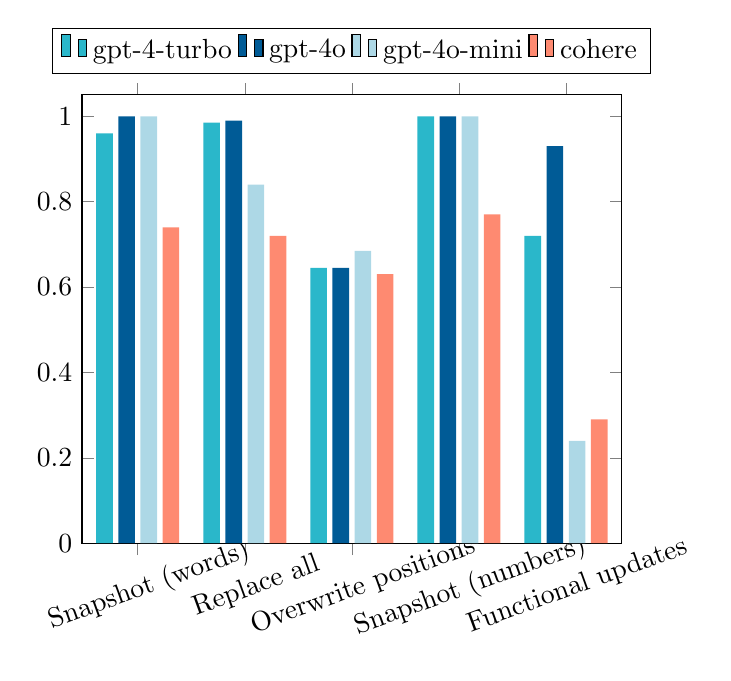
\begin{tikzpicture}
        \begin{axis}[
            ybar,
            bar width=6pt,
            symbolic x coords={Snapshot (words), Replace all, Overwrite positions, Snapshot (numbers), Functional updates},
            xtick=data,
            ymin=0, ymax=1.05,
            legend columns=4,
            legend style={at={(0.5,1.15)}, anchor=north, draw=black},
            enlarge x limits=0.13,
            xticklabel style={rotate=20, anchor=center, yshift=-12pt}
        ]
        
        \addplot[fill={rgb,255:red,42;green,183;blue,202}, draw=none] coordinates {(Snapshot (words),0.96) (Replace all,0.985) (Overwrite positions,0.645) (Snapshot (numbers),1.00) (Functional updates,0.72)};
        \addlegendentry{gpt-4-turbo}
        
        \addplot[fill={rgb,255:red,0;green,91;blue,150}, draw=none] coordinates {(Snapshot (words),1.00) (Replace all,0.99) (Overwrite positions,0.645) (Snapshot (numbers),1.00) (Functional updates,0.93)};
        \addlegendentry{gpt-4o}
        
        \addplot[fill={rgb,255:red,173;green,216;blue,230}, draw=none] coordinates {(Snapshot (words),1.00) (Replace all,0.84) (Overwrite positions,0.685) (Snapshot (numbers),1.00) (Functional updates,0.24)};
        \addlegendentry{gpt-4o-mini}
        
        \addplot[fill={rgb,255:red,254;green,138;blue,113}, draw=none] coordinates {(Snapshot (words),0.74) (Replace all,0.72) (Overwrite positions,0.63) (Snapshot (numbers),0.77) (Functional updates,0.29)};
        \addlegendentry{cohere}
        
        \end{axis}
\end{tikzpicture}}
    \end{subfigure}
    \begin{subfigure}{0.49\columnwidth}
        \resizebox{\textwidth}{!}{    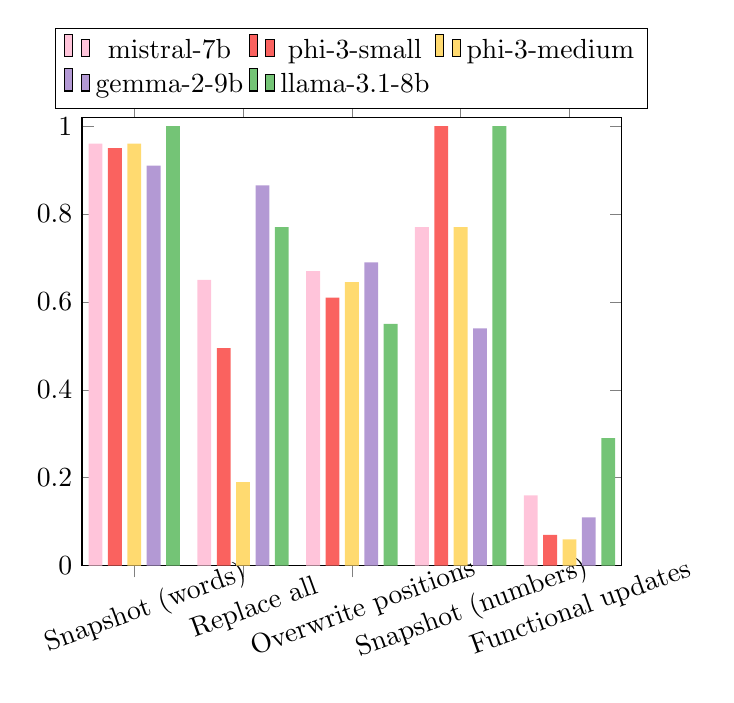
\begin{tikzpicture}
        \begin{axis}[
            ybar,
            bar width=5pt,
            symbolic x coords={Snapshot (words), Replace all, Overwrite positions, Snapshot (numbers), Functional updates},
            xtick=data,
            ymin=0, ymax=1.02,
            legend columns=3,
            legend style={at={(0.5,1.20)}, anchor=north, draw=black},
            enlarge x limits=0.12,
            xticklabel style={rotate=20, anchor=center, yshift=-12pt}
        ]
        
        \addplot[fill={rgb,255:red,255;green,196;blue,218}, draw=none] coordinates {(Snapshot (words),0.96) (Replace all,0.65) (Overwrite positions,0.67) (Snapshot (numbers),0.77) (Functional updates,0.16)};
        \addlegendentry{mistral-7b}
        
        \addplot[fill={rgb,255:red,250;green,98;blue,95}, draw=none] coordinates {(Snapshot (words),0.95) (Replace all,0.495) (Overwrite positions,0.61) (Snapshot (numbers),1.00) (Functional updates,0.07)};
        \addlegendentry{phi-3-small}
        
        \addplot[fill={rgb,255:red,255;green,218;blue,112}, draw=none] coordinates {(Snapshot (words),0.96) (Replace all,0.19) (Overwrite positions,0.645) (Snapshot (numbers),0.77) (Functional updates,0.06)};
        \addlegendentry{phi-3-medium}
        
        \addplot[fill={rgb,255:red,179;green,153;blue,212}, draw=none] coordinates {(Snapshot (words),0.91) (Replace all,0.865) (Overwrite positions,0.69) (Snapshot (numbers),0.54) (Functional updates,0.11)};
        \addlegendentry{gemma-2-9b}
        
        \addplot[fill={rgb,255:red,116;green,196;blue,118}, draw=none] coordinates {(Snapshot (words),1.00) (Replace all,0.77) (Overwrite positions,0.55) (Snapshot (numbers),1.00) (Functional updates,0.29)};
        \addlegendentry{llama-3.1-8b}
        
        \end{axis}
\end{tikzpicture}}
    \end{subfigure}
    \caption{Results for the \textbf{Recall and Edit} tasks.}
    \label{fig:recall}
\end{figure}

\paragraph{Recall and Edit} 
\begin{table}[!h]
    \centering
        \resizebox{0.8\columnwidth}{!}{%
    \begin{tabular}{lllll}
    \toprule
        \textbf{Model} & \textbf{String Search (word)} & \textbf{Snapshot} \\ \hline
gpt-4-turbo    & 1.00 \textcolor{green}{(0.06)} & 1.00 \textcolor{green}{(0.04)} \\ 
gpt-4o         & 1.00 (0.00)                   & 1.00 (0.00)                   \\ 
gpt-4o-mini    & 0.94 \textcolor{red}{(-0.04)}  & 1.00 (0.00)                   \\ 
cohere         & 1.00 (0.00)                   & 1.00 \textcolor{green}{(0.26)} \\ 
mistral-7b     & 1.00 \textcolor{green}{(0.22)} & 0.96 (0.00)                   \\ 
phi-3-small    & 1.00 \textcolor{green}{(0.06)} & 0.99 \textcolor{green}{(0.04)} \\ 
phi-3-medium   & 0.98 \textcolor{red}{(-0.02)}  & 0.87 \textcolor{red}{(-0.09)}  \\ 
gemma-2-9b     & 0.96 \textcolor{red}{(-0.04)}  & 0.96 \textcolor{green}{(0.05)} \\ 
llama-3.1-8b   & 0.98 \textcolor{red}{(-0.02)}  & 1.00 (0.00)                   \\
\bottomrule
    \end{tabular}
    }
    \caption{Ablation study with gibberish context.}
    \label{tab:ablation_gibberish}
\end{table}

Figure \ref{fig:recall} presents the results for the \textbf{Recall and Edit} tasks. While models performed well on basic recall (\textit{Snapshot}), their performance dropped sharply when tasked with making regular edits. A closer analysis of the generated outputs reveals that models struggled with maintaining coherence during edits, often getting trapped in repetitive word loops. For the \textit{Functional Update} task, we deliberately selected simple numerical updates, such as ``Subtract 1 from every number," to ensure the edits were within the models' capabilities. Nevertheless, when comparing performance on \textit{Snapshot (with numbers)} to \textit{Functional Updates}, all models exhibited a steep decline, especially for smaller ones. Analysis of generated outputs revealed that these models frequently deviated from instructions over longer sequences, suggesting difficulties in maintaining consistent rule applications over extended contexts.

Additionally, we conducted a separate ablation study on \textit{Snapshot} and \textit{String Search}. In this study, we replaced meaningful words in the context with gibberish tokens consisting of randomly generated alphabetical characters. As shown in Table \ref{tab:ablation_gibberish}, performance remained largely unchanged, suggesting that semantic meaning was not a significant distractor in these tasks.

\begin{table}
\centering
% \footnotesize
\resizebox{\linewidth}{!}{
\setlength{\tabcolsep}{5pt}
\begin{tabular}[t]{l|ccc}
\toprule
 \makecell[c]{\textbf{Method}} & \makecell[c]{\textbf{Self}\\\textbf{Reflection}} & \makecell[c]{\textbf{Memory}} & \makecell[c]{\textbf{Length}\\\textbf{Generalization}} \\
\midrule
Revision~\cite{DBLP:journals/corr/abs-2408-03314} & \redcross & \greencheck & \redcross \\
Self-Refine~\cite{DBLP:conf/nips/MadaanTGHGW0DPY23} & \greencheck & \greencheck & \redcross \\
Best-of-N~\cite{DBLP:journals/corr/abs-2407-21787} & \redcross & \redcross & \greencheck \\
Beam Search~\cite{ow1988filtered} & \redcross & \redcross & \greencheck \\
Guided Beam Search~\cite{DBLP:conf/nips/XieKZZKHX23} & \greencheck & \redcross & \greencheck \\
\midrule
\textbf{FTTT (ours)} & \greencheck & \greencheck & \greencheck \\
\bottomrule
\end{tabular}
}
% \vspace{-5pt}
\caption{Comparing the advantages and drawbacks of FTTT and related works.}
\label{tab:compare}
% \vspace{-0.5cm}
\end{table}

\begin{table}[!htbp] \centering
  \caption{Human Choices and Predictions About GenAI Choice in the Same Problem: Heterogeneity by Exposure and Attitudes (Pooled)}
\begin{adjustbox}{scale=0.8}
\begin{tabular}{@{\extracolsep{5pt}}lccccc}
% \\[-1.8ex]\hline
% \hline \\[-1.8ex]
\toprule
& \multicolumn{5}{c}{\textit{Dependent variable: Prediction}} \
\cr \cline{2-6}
\\[-1.8ex] & \multicolumn{1}{c}{Heavy User} & \multicolumn{1}{c}{Text-Based LLM User} & \multicolumn{1}{c}{Paid User} & \multicolumn{1}{c}{Agree AI Similar} & \multicolumn{1}{c}{Agree AI Better}  \\
\\[-1.8ex] & (1) & (2) & (3) & (4) & (5) \\
% \hline \\[-1.8ex]
\midrule
 X$\times$Heavy User & -0.056$^{}$ & & & & \\
& (0.052) & & & & \\
 X$\times$Text-Based LLM User & & 0.082$^{**}$ & & & \\
& & (0.040) & & & \\
 X$\times$Paid User & & & -0.001$^{}$ & & \\
& & & (0.072) & & \\
 X$\times$Agree AI Similar & & & & 0.033$^{}$ & \\
& & & & (0.045) & \\
 X$\times$Agree AI Better & & & & & 0.019$^{}$ \\
& & & & & (0.017) \\
 Problem FE & Yes & Yes & Yes & Yes & Yes \\
 X$\times$Problem FE & Yes & Yes & Yes & Yes & Yes \\
 G$\times$Problem FE & Yes & Yes & Yes & Yes & Yes \\
% \hline \\[-1.8ex]
\midrule
 Observations & 2700 & 2700 & 2700 & 2700 & 2700 \\
 % Residual Std. Error & 22.874 & 22.851 & 22.863 & 22.847 & 22.895 \\
% \hline
% \hline \\[-1.8ex]
\bottomrule
\textit{Note:} & \multicolumn{5}{r}{Standard errors are clustered at the problem level. $^{*}$p$<$0.1; $^{**}$p$<$0.05; $^{***}$p$<$0.01} \\
% \multicolumn{6}{r}\textit{} \\
\end{tabular}
\end{adjustbox}
\label{tab:group} \end{table}


\paragraph{Match and Compare}
 As shown in Figure \ref{fig:match}, model performance in the \textbf{Match and Compare} tasks was relatively consistent across different model sizes. Given that counting is a well-known weakness in LLMs, it is unsurprising that all models struggled significantly with the counting task, though GPT models performed slightly better than others. However, models generally succeeded in identifying the duplicates (in \textit{Find duplicates}), and primarily struggled with the counting aspect -- which requires tracking and updating an integer state, a skill that is more similar to stateful processing. This suggests that relying solely on counting-based tests \cite{song2024countingstars} could overly bias the evaluation and fail to capture broader model capabilities. The results also indicate that models exhibit some ability to recognize relative positions and group associations, but their accuracy remains limited (ranging between 0.6-0.8). A closer examination of model generations reveals an overwhelming tendency for the models to produce false positive errors -- models often answer “yes” when the correct answer is “no”, while making very few false negative errors. This means that when the relationship is correct, the models can more reliably identify it. This may stem from a combination of their inherent inclination to agree and the difficulty in recognizing relative comparisons and associations.

% \begin{figure}[h]
%     \centering
%     \includegraphics[width=0.92\columnwidth]{images/difference.png}
%     \caption{Results for \textbf{Spot the Differences }tasks.}
%     \label{fig:difference}
% \end{figure}

\begin{figure}[h]
\centering
\resizebox{0.9\columnwidth}{!}{
 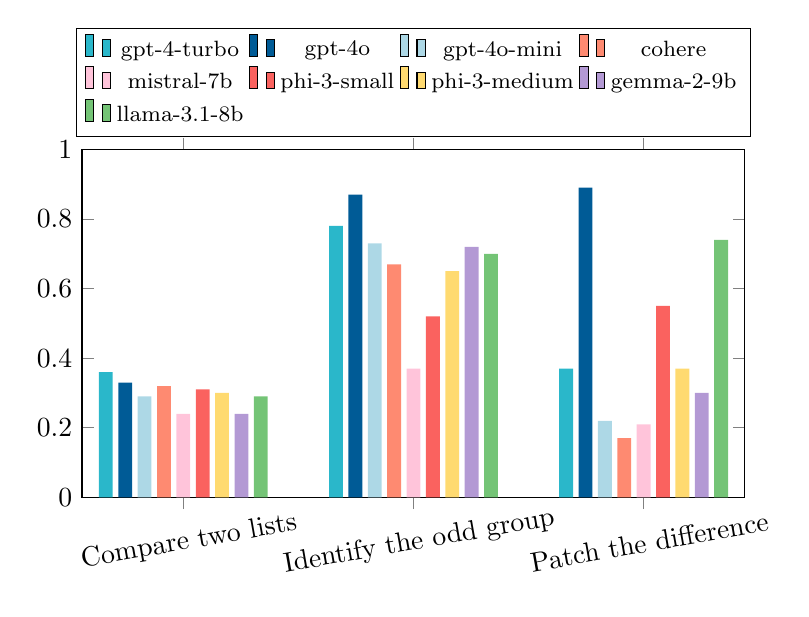
\begin{tikzpicture}
        \begin{axis}[
            ybar,
            bar width=5pt,
            symbolic x coords={Compare two lists, Identify the odd group, Patch the difference},
            xtick=data,
            ymin=0, ymax=1.0,
            legend columns=4,
            legend style={at={(0.5,1.35)}, anchor=north, draw=black, font=\footnotesize},
            enlarge x limits=0.22,
            xticklabel style={rotate=10, anchor=center, yshift=-12pt},
            width=10cm, height=6cm,
        ]
        
        \addplot[fill={rgb,255:red,42;green,183;blue,202}, draw=none] coordinates {(Compare two lists,0.36) (Identify the odd group,0.78) (Patch the difference,0.37)};
        \addlegendentry{gpt-4-turbo}
        
        \addplot[fill={rgb,255:red,0;green,91;blue,150}, draw=none] coordinates {(Compare two lists,0.33) (Identify the odd group,0.87) (Patch the difference,0.89)};
        \addlegendentry{gpt-4o}
        
        \addplot[fill={rgb,255:red,173;green,216;blue,230}, draw=none] coordinates {(Compare two lists,0.29) (Identify the odd group,0.73) (Patch the difference,0.22)};
        \addlegendentry{gpt-4o-mini}
        
        \addplot[fill={rgb,255:red,254;green,138;blue,113}, draw=none] coordinates {(Compare two lists,0.32) (Identify the odd group,0.67) (Patch the difference,0.17)};
        \addlegendentry{cohere}
        
        \addplot[fill={rgb,255:red,255;green,196;blue,218}, draw=none] coordinates {(Compare two lists,0.24) (Identify the odd group,0.37) (Patch the difference,0.21)};
        \addlegendentry{mistral-7b}
        
        \addplot[fill={rgb,255:red,250;green,98;blue,95}, draw=none] coordinates {(Compare two lists,0.31) (Identify the odd group,0.52) (Patch the difference,0.55)};
        \addlegendentry{phi-3-small}
        
        \addplot[fill={rgb,255:red,255;green,218;blue,112}, draw=none] coordinates {(Compare two lists,0.30) (Identify the odd group,0.65) (Patch the difference,0.37)};
        \addlegendentry{phi-3-medium}
        
        \addplot[fill={rgb,255:red,179;green,153;blue,212}, draw=none] coordinates {(Compare two lists,0.24) (Identify the odd group,0.72) (Patch the difference,0.30)};
        \addlegendentry{gemma-2-9b}
        
        \addplot[fill={rgb,255:red,116;green,196;blue,118}, draw=none] coordinates {(Compare two lists,0.29) (Identify the odd group,0.70) (Patch the difference,0.74)};
        \addlegendentry{llama-3.1-8b}
        
        \end{axis}
    \end{tikzpicture}}
    \caption{Results for \textbf{Spot the Differences }tasks.}
    \label{fig:difference}
\end{figure}

\paragraph{Spot the Differences}
As shown in Figure \ref{fig:difference}, performance across all models are poor on \textit{Compare Two Lists}, suggesting inherent difficulties in cross-referencing information across long contexts, even for larger models.  GPT-4o and the LLaMA model significantly outperform the others in the \textit{Identify the Odd Group} task, highlighting a general weakness in detecting contextual differences by the other models. However, an 8B LLaMA model outperforms both equivalently-sized models and even GPT-4 in this task, suggesting that model size alone was not the determining factor. This indicates that architectural differences, training objectives, or specific inductive biases may contribute to improved performance in comparative memory utilization.


\paragraph{Compute on Sets and Lists}
The tasks in this category require models to recognize and process group structures within the context, and performance gradually declines as the complexity of the task increases (see Table \ref{tab:lists}). For instance, in comparing the \textit{Group Membership} task with the \textit{String Search} task, where the former requires identifying which list a word belongs to rather than simply determining its presence, the performance of open-source models drops considerably. Similarly, in comparing the \textit{Group Association} task with the \textit{Group Membership} task, where the former requires determining whether two words belong to the same group, all models exhibit a noticeable decline in performance. The decline becomes even more pronounced when comparing the \textit{ Group Association (alternating)} variant of the task to the standard \textit{Group Association} task. Here, the context involves alternating repeated groups rather than simple group structures, which further challenges the models' abilities to handle partitioned contexts effectively.

An interesting observation was found during the \textit{Iterate} task. In an ablation study, we modified the task to require returning the first words in each list instead of the last words (making it more similar to the \textit{Batch Search} task). The performance sharply declines when models are asked to return the last words, despite their strong information-fetching capabilities. This suggests that, while the models can retrieve information effectively, they struggle to accurately recognize and process partitions within the context.



\begin{table}[t!]
\centering
    \resizebox{0.7\columnwidth}{!}{%

\begin{tabular}{lcc}
\toprule
\textbf{Model} & \textbf{Quantity state} & \textbf{Set state} \\
\midrule
gpt-4-turbo & 0.8 & \textbf{0.80} \\
gpt-4o & \textbf{1.0} & 0.65 \\
gpt-4o-mini & 0.7 & 0.24 \\
cohere & 0.0 & 0.58 \\
mistral-7b & 0.0 & 0.08 \\
phi-3-small & 0.0 & 0.13 \\
phi-3-medium & 0.0 & 0.11 \\
gemma-2-9b & 0.0 & 0.24 \\
llama-3.1-8b & 0.0 & 0.13 \\
\bottomrule
\end{tabular}
}
\caption{Results for \textbf{Stateful Processing} tasks.}
\label{tab:state}
\end{table}
\paragraph{Stateful Processing}

\begin{figure}[t!]
    \centering
    \begin{subfigure}{0.49\columnwidth}
        \resizebox{\textwidth}{!}{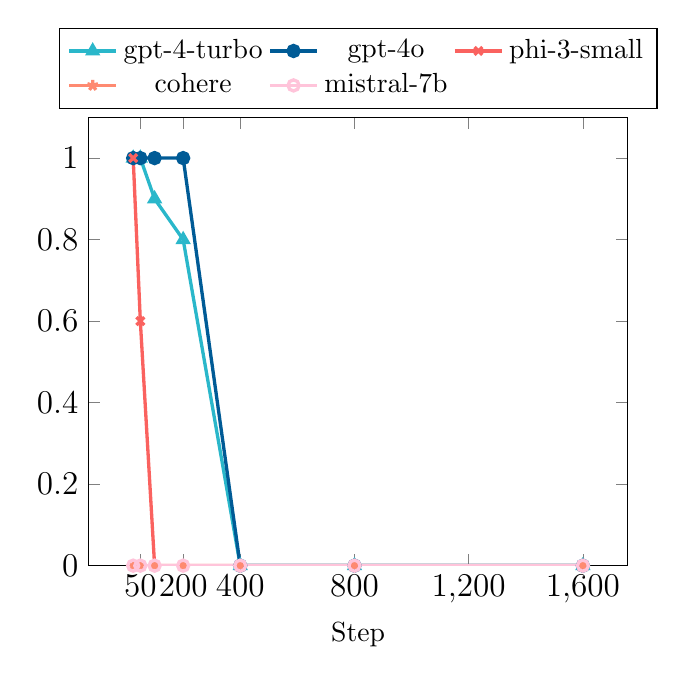
\begin{tikzpicture}
    \begin{axis}[
        xlabel={Step},
        legend style={at={(0.5,1.2)}, anchor=north, cells={align=left}, legend columns=3},
        ymin=0, ymax=1.1,
        xtick={50, 200, 400, 800, 1200, 1600},
        ytick={0,0.2,0.4,0.6,0.8,1.0},
        grid=none,
        tick label style={font=\large}
    ]

    % GPT-4-Turbo
    \addplot[mark=triangle, very thick, color={rgb,255:red,42;green,183;blue,202}] coordinates {
        (25,1.0) (50,1.0) (100,0.9) (200,0.8) (400,0.0) (800,0.0) (1600,0.0)
    };
    \addlegendentry{gpt-4-turbo}

    % GPT-4o
    \addplot[mark=*, very thick, color={rgb,255:red,0;green,91;blue,150}] coordinates {
        (25,1.0) (50,1.0) (100,1.0) (200,1.0) (400,0.0) (800,0.0) (1600,0.0)
    };
    \addlegendentry{gpt-4o}



    % Phi-3-Small
    \addplot[mark=x, very thick, color={rgb,255:red,250;green,98;blue,95}] coordinates {
        (25,1.0) (50,0.6) (100,0.0) (200,0.0) (400,0.0) (800,0.0) (1600,0.0)
    };
    \addlegendentry{phi-3-small}

    % Cohere
    \addplot[mark=star, very thick, color={rgb,255:red,254;green,138;blue,113}] coordinates {
        (25,0.0) (50,0.0) (100,0.0) (200,0.0) (400,0.0) (800,0.0) (1600,0.0)
    };
    \addlegendentry{cohere}

    % Mistral-7B
    \addplot[mark=o, very thick, color={rgb,255:red,255;green,196;blue,218}] coordinates {
        (25,0.0) (50,0.0) (100,0.0) (200,0.0) (400,0.0) (800,0.0) (1600,0.0)
    };
    \addlegendentry{mistral-7b}
    
    \end{axis}
\end{tikzpicture}}
    \end{subfigure}
    \begin{subfigure}{0.49\columnwidth}
        \resizebox{\textwidth}{!}{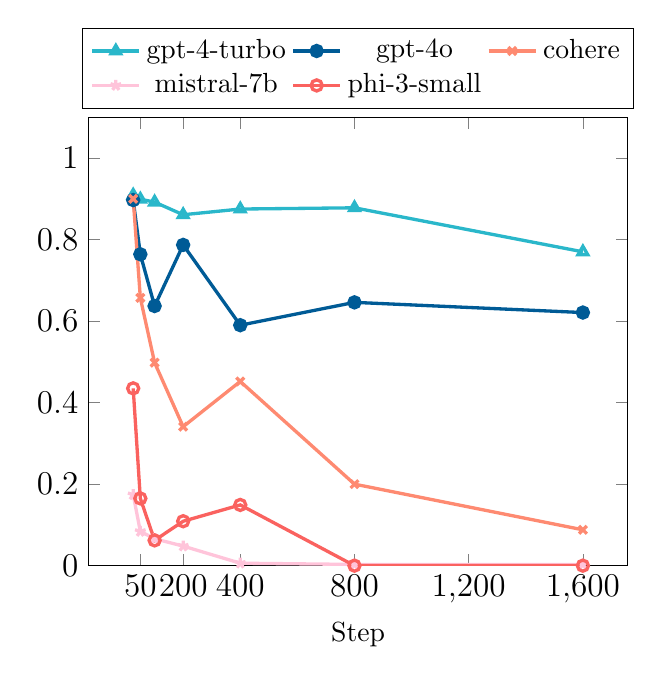
\begin{tikzpicture}
    \begin{axis}[
        xlabel={Step},
        legend style={at={(0.5,1.2)}, anchor=north, cells={align=left}, legend columns=3},
        ymin=0, ymax=1.1,
        xtick={50, 200, 400, 800, 1200, 1600},
        ytick={0,0.2,0.4,0.6,0.8,1.0},
        grid=none,
        tick label style={font=\large}
    ]

    % GPT-4-Turbo
    \addplot[mark=triangle, very thick, color={rgb,255:red,42;green,183;blue,202}] coordinates {
        (25,0.909) (50,0.899) (100,0.892) (200,0.861) (400,0.875) (800,0.878) (1600,0.770)
    };
    \addlegendentry{gpt-4-turbo}

    % GPT-4o
    \addplot[mark=*, very thick, color={rgb,255:red,0;green,91;blue,150}] coordinates {
        (25,0.897) (50,0.764) (100,0.637) (200,0.787) (400,0.590) (800,0.646) (1600,0.621)
    };
    \addlegendentry{gpt-4o}

    % Cohere
    \addplot[mark=x, very thick, color={rgb,255:red,254;green,138;blue,113}] coordinates {
        (25,0.900) (50,0.657) (100,0.498) (200,0.341) (400,0.452) (800,0.200) (1600,0.088)
    };
    \addlegendentry{cohere}

    % Mistral-7B
    \addplot[mark=star, very thick, color={rgb,255:red,255;green,196;blue,218}] coordinates {
        (25,0.174) (50,0.084) (100,0.066) (200,0.048) (400,0.006) (800,0.003) (1600,0.003)
    };
    \addlegendentry{mistral-7b}

    % Phi-3-Small
    \addplot[mark=o, very thick, color={rgb,255:red,250;green,98;blue,95}] coordinates {
        (25,0.435) (50,0.165) (100,0.062) (200,0.109) (400,0.149) (800,0.000) (1600,0.000)
    };
    \addlegendentry{phi-3-small}
    
    \end{axis}
\end{tikzpicture}}
    \end{subfigure}
    \caption{Ablation study on the number of operation steps for the \textbf{quantity state} (left) and\textbf{ set state }(right).}
    \label{fig:ablation_state_step}
\end{figure}



Table \ref{tab:state} presents the results for the \textbf{Stateful Processing} tasks, where performance gaps among models are the most pronounced. The GPT-4(o) models perform well on integer state tracking, while most other models struggle (near zero accuracy). For set state tracking, larger models generally perform better.

We conducted an ablation study to examine how the number of operation steps influences performance of five selected models (Fig. \ref{fig:ablation_state_step}). For quantity state tracking, GPT-4(o) models perform well within fewer than 200 steps but experience a sharp decline in accuracy beyond this threshold. For set state tracking, the performance decline is more gradual. The differences in performance drop between the two tasks can be attributed to the nature of the two tasks. While tracking an integer state might seem simpler than tracking a set, it actually requires the model to maintain and apply every operation sequentially to compute the final value. In contrast, for set state, the fixed size of the set makes more recent operations more relevant to the final state, reducing the need for exhaustive step-by-step tracking. Nevertheless, even in this scenario, all models show a clear inability to handle longer or more complex operation sequences effectively. Interestingly, GPT-4 model outperformed GPT-4o at this task, suggesting potential optimization trade-offs may have affected its ability to manage set-based updates. 

Overall, while larger models like GPT-4(o) exhibit some ability to track state over time, their effectiveness rapidly deteriorates as task complexity increases. Smaller models, in particular, struggle to track operations over time, pointing to significant gaps in their ability to manage and process sequential dependencies critical for state tracking tasks.

\subsection{Results on Composite Tests}

\section{Simple Construction of Projective Compositions}
\label{sec:comp_coord}

It is not clear apriori that projective compositional distributions satisfying Definition \ref{def:proj_comp} ever exist, much less that there is any straightforward way to sample from them.
To explore this, we first restrict attention to perhaps the simplest setting, where the projection functions $\{\Pi_i\}$ are
just coordinate restrictions.
This setting is meant to generalize the intuition we had
in the CLEVR example of Figure~\ref{fig:len_gen},
where different objects were composed in disjoint regions of the image.
We first define the construction of the composed distribution,
and then establish its theoretical properties.








\subsection{Defining the Construction}
Formally, suppose we have a set of distributions
$(p_1, p_2, \ldots, p_k)$ that we wish to compose;
in our running CLEVR example, each $p_i$ is the distribution of images
with a single object at position $i$.
Suppose also we have some reference distribution $p_b$,
which can be arbitrary, but should be thought of as a 
``common background'' to the $p_i$s.
Then, one popular way to construct a composed distribution
is via the \emph{compositional operator} defined below.
(A special case of this construction is used in \citet{du2023reduce}, for example).


\begin{definition}[Composition Operator]
    \label{def:comp_oper}
    Define the \emph{composition operator} $\cC$ acting on an arbitrary set of distributions $(p_b, p_1, p_2, \ldots)$ by
    \begin{align}
    \label{eq:comp_oper}
    \cC[\vec{p}] := \cC[p_b, p_1, p_2, \dots](x) := \frac{1}{Z} p_b(x) \prod_i \frac{p_i(x)}{p_b(x)},
    \end{align}
    where $Z$ is the appropriate normalization constant. We name $\cC[\vec{p}]$ the \emph{composed distribution}, and the score of $\cC[\vec{p}]$ the \emph{compositional score}:
    \begin{align}
    \label{eqn:comp_score}
    &\grad_x \log \cC[\vec{p}](x)  \\
    &= \grad_x \log p_b(x) + \sum_i \left( \grad_x \log p_i(x) - \grad_x \log p_b(x) \right). \notag
    \end{align}
\end{definition}
Notice that if $p_b$ is taken to be the unconditional distribution then this is exactly the Bayes-composition.


\vspace{-0.5em}
\subsection{When does the Composition Operator Work?}
We can always apply the composition operator to any set of distributions,
but when does this actually yield a ``correct'' composition
(according to Definition~\ref{def:proj_comp})?
One special case is when each distribution $p_i$ is
``active'' on a different, non-overlapping set of coordinates.
We formalize this property below
as \emph{Factorized Conditionals} (Definition~\ref{def:factorized}).
The idea is, 
each distribution $p_i$
must have a particular set of ``mask'' coordinates $M_i \subseteq [n]$ which it
samples in a characteristic way,
while independently sampling all other coordinates
from a common background distribution.
If a set of distributions $(p_b, p_1, p_2, \ldots)$ has this
\emph{Factorized Conditional} structure, then 
the composition
operator will produce a projective composition (as we will prove below).



\begin{definition}[Factorized-Conditionals]
\label{def:factorized}

We say a set of distributions $(p_b, p_1, p_2, \dots p_k)$
over $\R^n$
are \emph{Factorized Conditionals} if
there exists a partition of coordinates $[n]$
into disjoint subsets $M_b, M_1, \dots M_k$ such that:
\begin{enumerate}
    \setlength{\itemsep}{1pt}
    \item $(x|_{M_i}, x|_{M_i^c})$ are independent under $p_i$.
    \item $(x|_{M_b}, x|_{M_1}, x|_{M_2}, \dots, x|_{M_k})$
    are mutually independent under $p_b$.
    \item $p_i(x|_{M_i^c}) = p_b(x|_{M_i^c})$.
\end{enumerate}

Equivalently, if we have:
\begin{align}
    p_i(x) &= p_i(x|_{M_i}) p_b(x|_{M_i^c}), \text{ and} \label{eqn:cc-cond}\\
    p_b(x) &= p_b(x|_{M_b}) \prod_{i \in [k]} p_b(x|_{M_i}). \notag
\end{align}
\end{definition}
\vspace{-1em}
Equation~\eqref{eqn:cc-cond} means that each $p_i$
can be sampled by first sampling $x \sim p_b$,
and then overwriting the coordinates of $M_i$
according to some other distribution (which can be specific to distribution $i$).
For instance, the experiment of Figure~\ref{fig:len_gen}
intuitively satisfies this property, since 
each of the conditional distributions could essentially be sampled
by first sampling an empty background image ($p_b$), then ``pasting''
a random object in the appropriate location (corresponding to pixels $M_i$).
If a set of distributions obey this Factorized Conditional structure,
then we can prove that the composition operator $\cC$
yields a correct projective composition,
and reverse-diffusion correctly samples from it.
Below, let $N_t$ denote the noise operator of the
diffusion process\footnote{Our results are agnostic to the specific diffusion noise-schedule and scaling used.} at time $t$.

\begin{theorem}[Correctness of Composition]
\label{lem:compose}
Suppose a set of distributions $(p_b, p_1, p_2, \dots p_k)$
satisfy Definition~\ref{def:factorized},
with corresponding masks $\{M_i\}_i$.
Consider running the reverse-diffusion SDE 
using the following compositional scores at each time $t$:
\begin{align}
s_t(x_t) &:= \grad_x \log \cC[p_b^t, p_1^t, p_2^t, \ldots](x_t),
\end{align}
where $p_i^t := N_t[p_i]$ are the noisy distributions.
Then, the distribution of the generated sample $x_0$ at time $t=0$ is:
\begin{align}
\label{eqn:p_hat}
\hat{p}(x) := p_b(x|_{M_b}) \prod_i p_i(x|_{M_i}).
\end{align}
In particular,
$\hat{p}(x|_{M_i}) = p_i(x|_{M_i})$ for all $i$,
and so
$\hat{p}$ is a projective composition
with respect to projections $\{\Pi_i(x) := x|_{M_i}\}_i$,
per Definition \ref{def:proj_comp}.
\end{theorem}




Unpacking this, Line \ref{eqn:p_hat} says that the final generated distribution
$\hat{p}(x)$ can be sampled by
first sampling
the coordinates $M_b$ according to $p_b$ (marginally),
then independently sampling 
coordinates $M_i$ according to $p_i$ (marginally) for each $i$.
Similarly, by assumption, $p_i(x)$ can be sampled by first sampling the coordinates $M_i$ in some specific way, and then independently sampling the remaining coordinates according to $p_b$. Therefore Theorem \ref{lem:compose} says that $\hat{p}(x)$ samples the coordinates \emph{$M_i$ exactly as they would be sampled by $p_i$}, for each $i$ we wish to compose. 

\begin{proof}(Sketch) \small
Since $\vec{p}$ satisfies Definition \ref{def:factorized}, we have
\begin{align*}
&\cC[\vec{p}](x) := p_b(x) \prod_i \frac{p_i(x)}{p_b(x)} \notag 
= p_b(x) \prod_i \frac{p_b(x_t|_{M_i^c}) p_i(x|_{M_i})}{p_b(x|_{M_i^c})p_b(x|_{M_i})} \notag \\
&= p_b(x) \prod_i \frac{p_i(x|_{M_i})}{p_b(x|_{M_i})} \notag 
= p_b(x|_{M_b}) \prod_i p_i(x_t|_{M_i}) := \hat{p}(x).
\end{align*}
The sampling guarantee follows from the commutativity of composition with the diffusion noising process, i.e. $\cC[\vec{p^t}]= N_t[\cC[\vec{p}]]$. 
The complete proof is in Appendix \ref{app:compose_pf}.
\end{proof}

\begin{remark}
In fact, Theorem~\ref{lem:compose} still holds under any orthogonal transformation of the variables,
because the diffusion noise process commutes with orthogonal transforms.
We formalize this as Lemma~\ref{lem:orthogonal_sampling}.
\end{remark}

\begin{remark}
Compositionality is often thought of in terms of orthogonality between scores.
Definition \ref{def:factorized} implies orthogonality between the score differences that appear in the composed score \eqref{eqn:comp_score}:
$\grad_x \log p_i^t(x_t) - \grad_x \log p_b^t(x_t),$
but the former condition is strictly stronger
(c.f. Appendix \ref{app:score_orthog}).
\end{remark}

\begin{remark}
Notice that the composition operator $\cC$
can be applied to a set of Factorized Conditional
distributions
without knowing the coordinate partition $\{M_i\}$.
That is, we can compose distributions and compute scores
without knowing apriori exactly ``how'' these distributions are supposed to compose
(i.e. which coordinates $p_i$ is active on).
This is already somewhat remarkable, and we will see a much
stronger version of this property in the next section.
\end{remark}

\textbf{Importance of background.}
Our derivations highlight the crucial role of the background
distribution $p_b$ for the composition operator  
(Definition~\ref{def:comp_oper}).
While prior works have taken $p_b$ to be an unconditional distribution and the $p_i$'s its associated conditionals,
our results suggest this is not always the optimal choice -- in particular,
it may not satisfy a Factorized Conditional structure (Definition~\ref{def:factorized}). Figure~\ref{fig:len_gen_monster} demonstrates this empirically: settings (a) and (b) attempt to compose the same distributions using different backgrounds -- empty (a) or unconditional (b) -- with very different results.

\subsection{Approximate Factorized Conditionals in CLEVR.}
\label{sec:clevr-details}

In \cref{fig:len_gen_monster} we explore compositional length-generalization (or lack thereof) in three different setting, two of which (\cref{fig:len_gen_monster}a and \ref{fig:len_gen_monster}c) approximately satisfy \cref{def:factorized}. In this section we explicitly describe how our definition of Factorized Conditionals approximately captures the CLEVR settings of Figures \ref{fig:len_gen_monster}a and \ref{fig:len_gen_monster}c. The setting of \ref{fig:len_gen_monster}b does not satisfy our conditions, as discussed in \cref{sec:problematic-compositions}.

\textbf{Single object distributions with empty background.}
This is the setting of both \cref{fig:len_gen} and \cref{fig:len_gen_monster}a.
The background distribution $p_b$ 
over $n$ pixels is images of an empty scene with no objects.
For each $i \in \{1,\ldots,L\}$ (where $L=4$ in \cref{fig:len_gen} and $L=9$ in \cref{fig:len_gen_monster}a), define the set $M_i \subset [n]$ 
as the set of pixel indices surrounding location $i$.
($M_i$ should be thought of as a ``mask'' that
that masks out objects at location $i$).
Let $M_b := (\cup_i M_i)^c$ be the remaining
pixels in the image.
Then, we claim the distributions $(p_b, p_1, \ldots, p_L)$
form approximately
Factorized Conditionals, with corresponding
coordinate partition $\{M_i\}$.
This is essentially because each distribution $p_i$
matches the background $p_b$ on all pixels except those surrounding
location $i$ (further detail in Appendix~\ref{app:clevr-details}).
Note, however, that the conditions of Definition~\ref{def:factorized}
do not \emph{exactly} hold in the experiment of Figure~\ref{fig:len_gen} -- there is still some dependence between
the masks $M_i$, since objects can cast shadows or even occlude each other.
Empirically, these deviations 
have greater impact
when composing many objects, as seen in \cref{fig:len_gen_monster}a.


\textbf{Bayes composition with cluttered distributions.}
In \cref{fig:len_gen_monster}c we replicate CLEVR experiments in  \citet{du2023reduce, liu2022compositional} where the images contain many objects (1-5) and the conditions label the location of one randomly-chosen object. It turns out the unconditional together with the conditionals can approximately act as Factorized Conditionals in ``cluttered'' settings like this one. The intuition is that if the conditional distributions each contain one specific object plus many independently sampled random objects (``clutter''), then the unconditional distribution \emph{almost} looks like independently sampled random objects, which together with the conditionals \emph{would} satisfy Definition \ref{def:factorized} (further discussion in Appendix \ref{app:clevr-details} and \ref{app:bayes_connect}). This helps to explain the length-generalization observed in \citet{liu2022compositional} and verified in our experiments (\cref{fig:len_gen_monster}c).







\section{Projective Composition in Feature Space}
\label{sec:comp_feature}

\begin{figure}
    \centering
    \includegraphics[width=1.0\linewidth]{figures/feat-space-vis.png}
    \caption{A commutative diagram illustrating Theorem~\ref{lem:transform_comp}.
    Performing composition in pixel space is equivalent 
    to encoding into a feature space ($\cA$),
    composing there,
    and decoding back
    to pixel space ($\cA^{-1}$).
    }
    \label{fig:feat-space-vis}
\end{figure}

So far we have focused on the setting where the projection functions $\Pi_i$ are simply projections onto coordinate subsets $M_i$ in the native space (e.g. pixel space).
This covers simple examples like Figure~\ref{fig:len_gen} but does not include more realistic situations such as Figure~\ref{fig:style-content},
where the properties to be composed are more abstract.
For example a property like ``oil painting'' does not correspond to projection
onto a specific subset of pixels in an image.
However, we may hope that there exists some conceptual feature space
in which ``oil painting'' does correspond to a particular subset of variables.
In this section, we extend our results to the case where the composition occurs in some conceptual feature space, and each distribution to be composed
corresponds to some particular subset of \emph{features}.


Our main result is a featurized analogue of Theorem~\ref{lem:compose}:
if there exists \emph{any} invertible transform $\cA$
mapping into a feature space
where Definition \ref{def:factorized} holds,
then the composition operator (Definition~\ref{def:comp_oper})
yields a projective composition in this feature space, as shown in Figure~\ref{fig:feat-space-vis}.

\begin{theorem}[Feature-space Composition]
\label{lem:transform_comp}
Given distributions $\vec{p} := (p_b, p_1, p_2, \dots p_k)$,
suppose there exists a diffeomorphism $\cA: \R^n \to \R^n$
such that
$(\cA \sharp p_b, \cA \sharp p_1, \dots \cA \sharp p_k)$
satisfy Definition~\ref{def:factorized},
with corresponding partition $M_i \subseteq [n]$.
Then, the composition $\hat{p} := \cC[\vec{p}]$ satisfies:
\begin{align}
\label{eqn:p_hat_A}
\cA \sharp \hat{p}(z)
\equiv
(\cA \sharp p_b (z))|_{M_b} \prod_{i=1}^k (\cA \sharp p_i(z))|_{M_i}.
\end{align}
Therefore, $\hat{p}$
is a projective composition of $\vec{p}$ w.r.t. projection functions
$\{\Pi_i(x) := \cA(x)|_{M_i}\}$.
\end{theorem}
This theorem is remarkable because it means we can
compose distributions $(p_b, p_1, p_2, \dots)$ in the base space,
and this composition will ``work correctly'' in the feature space
automatically (Equation~\ref{eqn:p_hat_A}),
without us ever needing to compute or even know the feature transform $\cA$
explicitly.



Theorem~\ref{lem:transform_comp} may apriori seem too strong
to be true, since it somehow holds for all feature spaces $\cA$
simultaneously.
The key observation underlying Theorem~\ref{lem:transform_comp} 
is that the composition operator $\cC$ behaves
well under reparameterization.
\begin{lemma}[Reparameterization Equivariance]
\label{lem:reparam}
The composition operator of Definition~\ref{def:comp_oper}
is reparameterization-equivariant. That is,
for all diffeomorphisms $\cA: \R^n \to \R^n$
and all tuples of distributions $\vec{p} = (p_b, p_1, p_2, \dots, p_k)$,
\begin{align}
 \cC[ \cA \sharp \vec{p}] =  \cA \sharp \cC[\vec{p}].
\end{align}
\end{lemma}
\arxiv{\footnote{
For example (separate from our goals in this paper):
Classifier-Free-Guidance can be seen as an instance of the composition operator.
Thus, Lemma~\ref{lem:reparam} implies that performing CFG
in latent space is \emph{equivalent} to CFG in pixel-space,
assuming accurate score-models in both cases.}}
\arxiv{This lemma is potentially of independent interest:
reparametrization-equivariance
is a very strong property which is typically not satisfied by
standard operations between probability distributions---
for example, the ``simple product'' $p_1(x)p_2(x)$ does not satisfy it---
so it is mathematically notable that the composition operator 
has this structure.
Lemma~\ref{lem:reparam} and Theorem~\ref{lem:transform_comp}
are proved in Appendix \ref{app:param-indep}.}

This lemma is potentially of independent interest:
equivariance distinguishes the composition operator
from many other common operators
(e.g. the simple product).
Lemma ~\ref{lem:reparam} and Theorem~\ref{lem:transform_comp}
are proved in Appendix \ref{app:param-indep}.

\section{Sampling from Compositions.}
The feature-space Theorem~\ref{lem:transform_comp} is weaker than Theorem~\ref{lem:compose}
in one important way: it does not provide a sampling algorithm.
That is, Theorem~\ref{lem:transform_comp} guarantees that $\hat{p} := \cC[\vec{p}]$
is a projective composition, but does not guarantee that reverse-diffusion
is a valid sampling method.

There is one special case where diffusion sampling \emph{is} guaranteed to work, namely, for orthogonal transforms (which can seen as a straightforward extension of the coordinate-aligned case of \cref{lem:compose}):
\begin{lemma}[Orthogonal transform enables diffusion sampling]
\label{lem:orthogonal_sampling}
If the assumptions of Lemma \ref{lem:transform_comp} hold for $\cA(x) = Ax$, where $A$ is an orthogonal matrix, then running a reverse diffusion sampler with scores $s_t = \grad_x \log \cC[\vec{p}^t]$ generates the composed distribution $\hat{p} = \cC[\vec{p}]$ satisfying \eqref{eqn:p_hat_A}.
\end{lemma}
The proof is given in \cref{app:orthog_sample_pf}.

However, for general invertible transforms, we have no such sampling guarantees.
Part of this is inherent: in the feature-space setting, the 
diffusion noise operator $N_t$ no longer commutes
with the composition operator $\cC$ in general,
 so scores of the noisy composed 
distribution $N_t[\cC[\vec{p}]]$
cannot be computed from scores
of the noisy base distributions $N_t[\vec{p}]$.
Nevertheless, one may hope to sample from the distribution $\hat{p}$
using other samplers besides diffusion, 
such as annealed Langevin Dynamics
or
Predictor-Corrector methods \citep{song2020score}.
We find that the situation is surprisingly subtle:
composition $\cC$ produces distributions which
are in some cases easy to sample (e.g. with diffusion),
yet in other cases apparently hard to sample.
For example, in the
setting of Figure~\ref{fig:clevr_color_comp}, 
our Theorem~\ref{lem:transform_comp} implies
that all pairs of colors should compose equally well
at time $t=0$, since there exist diffeomorphisms
(indeed, linear transforms) between different colors.
However, as we saw,
the diffusion sampler
fails to sample from compositions 
of non-orthogonal colors--- and 
empirically, even more sophisticated
samplers such as Predictor-Correctors
also fail in this setting.
At first glance, it may seem odd that
composed distributions are so hard to sample,
when their constituent distributions are relatively easy to sample.
One possible reason for this below is that the composition operator has extremely poor Lipchitz constant,
so it is possible for a set of distributions $\vec{p}$ to ``vary smoothly''
(e.g. diffusing over time) while their composition $\cC[\vec{p}]$
changes abruptly.
We formalize this in \cref{lem:lipschitz} (further discussion and proof in Appendix \ref{app:lipschitz}).
\begin{lemma}[Composition Non-Smoothness]
\label{lem:lipschitz}
For any set of distributions $\{p_b, p_1, p_2, \dots, p_k\}$,
and any noise scale $t := \sigma$,
define the noisy distributions 
$p_i^t := N_{t}[p_i]$,
and let $q^t$ denote the composed distribution at time $t$: $q^t := \cC[\vec{p}^t]$. Then, for any choice of $\tau > 0$,
there exist distributions $\{p_b, p_1, \dots p_k\}$ over $\R^n$
such that
\begin{enumerate}
    \setlength{\itemsep}{0pt}
    \item For all $i$, the annealing path of $p_i$ is 
    $\cO(1)$-Lipshitz:
    $\forall t, t': W_2(p_i^{t}, p_i^{t'}) \leq \cO(1) |t - t'|$.
    \item The annealing path of $q$ has Lipshitz constant
    at least $\Omega(\tau^{-1})$:
    $\exists t, t': W_2(q^{t}, q^{t'}) \geq \frac{|t - t'|}{2\tau}.$
\end{enumerate}
\end{lemma}




The composite tests significantly challenge the models by combining multiple atomic capabilities into a single test. In the \textit{Processing Data Blocks} task, the context is fixed at 4k tokens, while for the \textit{Theory of Mind} task, the number of operation steps is set to 100. As shown in Table \ref{tab:comp}, model performance on both tasks are generally low, showing a broad inability to handle the more complex scenarios. Performance across all models drop substantially on composite tasks compared to their performance on individual capability tasks, such as search, recall, and group processing. 

Interestingly, some smaller models, like Mistral and Phi-3-small, exhibit slightly better performance on the \textit{Theory of Mind} task than on the set state tracking task. This anomaly likely stems from their already weak state tracking ability, which limits their performance across both tasks. Additionally, these models tend to generate longer answers in the set state task which reduces the set overlap.

Notably, even the most capable models, such as GPT-4-turbo and GPT-4o, struggle, showing that scaling model size alone is not enough for solving these composite tasks. Additionally, the variation in performance among smaller models suggests that their limitations stem not only from size but also from underlying architectural or training differences. This indicates that smaller models require more targeted care to bridge the gap in effective memory use.



% \section{Research Questions}
% \label{sec:rq}

% Introduce your research questions briefly
\setlength{\parskip}{0pt}

\section{Quantitaive Analysis}
\label{sec:study}



% Please add the following required packages to your document preamble:
% \usepackage{booktabs}
\begin{table}[]
\caption{Pass@1 (\%) scores for various SOTA LLMs on DS-1000 and \tool.}
\label{tab:RQ1_ACC}
\center
\resizebox{0.6\linewidth}{!}{
\begin{tabular}{llr}
\toprule
\textbf{Benchmark}                                      & \textbf{LLM}              & \textbf{Pass@1} \\ 
\midrule
\multirow{4}{*}{DS-1000}& GPT-4o           & 60\\
 & Claude 3.5 sonnet&54\\
 & LLama 3.1 70B&41\\
 & Mistral 7B&20\\
%\multicolumn{1}{l}{\multirow{4}{*}{DS-1000}} & GPT 4o           & 0.20   \\
%\multicolumn{1}{c}{}                         & Claude 3.5 sonet & 0.18   \\
%\multicolumn{1}{c}{}                         & LLama 3.1 70B    & 0.17   \\
%\multicolumn{1}{c}{}                         & Mistral 7B       & $<$0.01  \\ 
\midrule
\multicolumn{1}{l}{\multirow{4}{*}{\tool}}  & GPT-4o           & 31   \\
\multicolumn{1}{c}{}                         & Claude 3.5 sonnet & 28   \\
\multicolumn{1}{c}{}                         & LLama 3.1 70B    & 21   \\
\multicolumn{1}{c}{}                         & Mistral 7B       & 15   \\
\bottomrule
\end{tabular}
}
\end{table}


\textbf{What are the performances of SOTA LLMs on DL/ML code generation tasks?}
In this analysis, we investigate how the existing ML code generation benchmark (DS-1000) and \tool evaluate SOTA LLMs.
Table~\ref{tab:RQ1_ACC} shows the pass@1 metric of SOTA LLMs on those benchmarks.
%specifically designed to test code generation capabilities. The dataset consists of carefully crafted prompts or doc-strings to minimize the risk of memorization by the LLM. 
To focus on 
%the purpose of this RQ is to 
demonstrating \tool's ability to evaluate existing LLMs, we intentionally avoided using specialized prompt strategies, opting instead for vanilla prompts to assess the model's baseline performance. However, the use of advanced prompt engineering strategies could yield different results and this will be interesting for future usage of \tool. 

Our analysis underscores that even the most advanced model such as GPT-4o struggles with ML/DL-specific code generation. Specifically, GPT-4o achieves only 60\% and 31\% Pass@1 scores on DS-1000 and \tool respectively. 
Also, when comparing between DS-1000 and \tool, our benchmark is more challenging as the SOTA LLM gets a much lower Pass@1 score, SOTA LLMs in other categories are behind GPT-4o with performance as low as 15\% for the tiny Mistral 7B model on \tool. The overall weak performance of these models highlights the ongoing challenges in generating reliable, executable ML/DL code which supports the need for more benchmarks in this domain.

%\hung{do we have any idea how our run of ds-1000 is much lower than their run? Was it because of pass@k where k is not 1? Or do they have special dependencies that we need to set up? It is kind of bad if they say they get 53\% but we get 20\%, to the reader, this will effect their confidence in our work.}
%\alireza{I used exactly run their scrips and build the environment as they set. I can mail them and ask}
%\hung{yes, for now I will just include their reported value.}

%Our analysis underscores that even the most advanced models struggle with code generation for deep learning %tasks. GPT-4, while performing best, still only achieves a Pass@1 score of 0.31 This reflects a broader trend—none of the models truly excel. Claude 3.5 and LLaMA 3.1, though slightly behind GPT-4o, also fail to meet expectations. Mistral, the weakest, falls significantly short of the benchmark. The overall weak performance of these models highlights the ongoing challenges in generating reliable, executable code.

% \hung{can we have the passing rate analysis there?}

% \hung{Also compilation rate or syntact error rate? This would be very interesting to discuss here.}

Overall, GPT-4o's pass@k is 31\%, but to further assess its performance, we calculated the average passing rate across the functions, which was higher at 40\%. This suggests that while only 31\% of functions pass all test cases, many pass some. With additional insights, these partially valid cases could be improved.

%the overall pass@k metric may appear lower, the model demonstrates improved performance in specific scenarios when evaluated on a case-by-case basis.

%For example, more advanced prompt techniques can be used to improve the result. Such techniques often require additional domain-specific information from deeper analyses that DS-1000 could not provide. In the later RQs, we will demonstrate how \tool can be used to conduct deep analyses so useful insights can be extracted and more sophisticated prompting techniques can be developed to better tackle the task of generating DL-specific code.

%To improve these outcomes, future experiments might explore optimized prompting strategies, such as prompt tuning or providing more detailed context. These approaches could potentially enhance the performance of GPT-4o in complex code generation tasks, particularly those within the AI domain. Our current findings suggest that while GPT-4o demonstrates some level of competence, its application in practical AI code generation remains limited without further optimization.

\begin{tcolorbox}[boxrule=0.5pt, colback=gray!10,  arc=4pt,left=3pt,right=3pt,top=3pt,bottom=3pt,boxsep=0pt
]
\textbf{Finding 1:} Our evaluation indicates that current LLMs struggle to generate correct, executable code for ML/DL tasks. Although GPT-4o is the strongest among the tested models, it still falls short of meeting practical standards (Pass@k score of only 31\%). 
%Prior benchmarks such as DS-1000 pose some challenges to the top SOTA LLM but are still not as challenging as \tool. 
A deeper analysis is needed (which \tool can provide) to extract insight into improving prompting techniques.
%This underscores the limitations of existing LLMs in AI code generation and highlights the need for optimized prompting strategies or further advancements to enhance their performance.
\end{tcolorbox}

% \begin{tcolorbox}[boxrule=0.5pt, colback=gray!10, arc=4pt,left=6pt,right=6pt,top=6pt,bottom=6pt,boxsep=0pt]
% \textbf{Finding 1:} Our findings suggest that task complexity, data variability, and the nature of the input are critical factors in determining how well an LLM can generate accurate code. These insights shed light on the current limitations of LLMs and provide direction for future research aimed at improving their performance in more complex domains, such as image segmentation.
% \end{tcolorbox}

\begin{table}[]
\caption{Pass@1 scores (\%) for different LLMs in different stages on \tool}
\label{tab:RQ2_MLStage}
\resizebox{\linewidth}{!}{
\begin{tabular}{@{}l@{}rrrrr@{}}
\toprule
\textbf{Model}                        & \makecell{ \textbf{Pre/Post} \\ \textbf{Processing} }    & \makecell{ \textbf{Model} \\ \textbf{Construction}} & \textbf{Training}              & \textbf{Inference}            & \makecell{ \textbf{Evaluation} \\ \textbf{\& Metrics} }  \\ \midrule
GPT-4o           & \textbf{33} & \textbf{26} & \textbf{31} & 30&\textbf{32} \\
Claude 3.5 sonnet & 31 & 22 & 28 & 30& 29 \\
LLama 3.1 70B    & 22 & 14 & 21 & 29 & 24 \\
Mistral 7B          & 14 & 11& 16& 26 & 19 \\
\bottomrule
\end{tabular}
}
\end{table}


\textbf{Which stages in the ML pipeline pose a greater challenge for SOTA LLMs?}
We conduct an analysis of the challenges of generating DL code for specific stages in the pipeline (enabled by %Since 
\tool provided categorization)
%of the stage that each of our data points belongs to in the ML pipeline, we group the result into these specific stages. T
Table~\ref{tab:RQ2_MLStage} presents the Pass@1 scores that each LLM achieves for code in each %categorization of 
ML/DL pipeline stage.
Our result shows that the best SOTA LLM---GPT-4o---outperforms all of the other LLMs in all stages. Claude 3.5 sonnet is the closest second, where in the \textit{Inference} category, it is level with GPT-4o. 

%We tested our benchmark using SOTA LLMs, focusing on its ability to perform tasks across these different stages. By examining the model's performance in each category, we aim to identify the specific challenges and complexities involved in generating the various pipeline steps. This analysis will provide valuable insights into the strengths and limitations of different LLMs when applied to different tasks within the AI pipeline.

%\begin{figure}
    \centering
    \includegraphics[width=\linewidth]{figs/box_x.pdf}
    %\vspace{-7pt}
    \caption{Pre/post processing example: Converting formats of bounding boxes
    }
    \label{fig:accepted1}
    %\vspace{-10pt}
\end{figure}
\textit{Pre/post Processing} stages often require small but important data transformation tasks, thus such codes are the most available. Hence, 
%in AI and deep learning projects where 
\tool collected the most data in this category (210/520). %This is because many different tasks are performed on the data at the beginning (pre-processing) or at the end (post-processing) of the pipeline. 
Code in this category prepares and cleans the input data for the model and formats the model's output. 
%For example, the prompt and reference code in Fig~\ref{fig:accepted1} demonstrate a straightforward task of converting the format of the bounding boxes which is common in image-processing ML systems.
Our result shows that LLMs have the most success in generating code for 
%this case.
the Pre/post Processing stages. 
One possible reason for the higher Pass@1 scores is that the models might have more changes to learn from a vast set of samples in this category. 
%of such 
%pre/post processing category.
%tasks in their respective training sets. 

%The reason LLMs, usually perform better in pre- and post-processing might be to do with the higher number of related code samples to these tasks, in the training set. Pre- and post-processing involve common tasks(e.g., \ref{fig:accepted1} which GPT 4o generated correct code for that which is a simple pre/post-processing task that easily transforms bounding box coordinates) that are used in many projects, making them easier for LLMs to predict and generate accurately. In addition, the code for these stages is usually more repetitive, which helps the models handle them more effectively.

On the other hand, LLMs struggle to generate code for the \textit{Model Construction} stage with the
%showed the 
lowest Pass@1 scores.
%in our experiments. 
This is because the code for this stage is more complex, very project-specific, and often longer.
%is usually much longer and more complex. Unlike pre and post-processing, model construction is unique to each project, making it harder for GPT-4o to generate accurate code.

%\begin{figure}
    \centering
    \includegraphics[width=\linewidth, ]{figs/cauchy_last.pdf}
    %\vspace{-7pt}
    \caption{Model Construction example
    }

    \label{fig:rejected2}
    %\vspace{-10pt}
\end{figure}
%\subsection{Superpixel Segmentation} \label{sec:segmentation}

Superpixels are perceptually meaningful, connected regions that group pixels based on similarities in color or other features, first introduced by \citet{renmalik2003}. Since then, various algorithmic approaches have been developed \citep{achanta2012, felzenszwalb2004}. Defining appropriate local regions is crucial for extracting spatial features in spectral-spatial models. While fixed-size windows (e.g., \citet{ertem2020}) have shown promising results, they constrain the ability to fully capture spatial context. In contrast, superpixels provide adaptive regions that enhance discriminative information, as demonstrated by \citet{fang2015kernals}. \citet{cui2018} further highlighted this by employing a superpixel-based random walker to refine an SVM probability map with significant success. Additionally, Cui et al. showed that superpixel spectra are more stable and less sensitive to noise than individual pixel spectra, making superpixel-based approaches more robust to image noise.


% The most common algorithm used in clustering based superpixel methods is Lloyd's algorithm \citep{lloyd2006}, a modified version of the popular k-means clustering algorithm. In the context of Lloyd's algorithm, let us first formalise the definition of a superpixel segmentation.

\begin{definition}[Superpixel Segmentation]  
Given an image \( I : \Lambda \to \mathbb{R}^d \), where \( \Lambda \subset \mathbb{Z}^2 \) represents the image domain, superpixel segmentation partitions \( \Lambda \) into a set of regions \(\{S_i\}_{i=1}^n\). Each superpixel \( S_i \) is defined as \( S_i = \{x \in \Lambda : f(x) = i\} \), where \( f: \Lambda \to \{1, \ldots, n\} \) is a labeling function that assigns each pixel \( x \) to one of the \( n \) superpixels based on a feature function.  
\end{definition}


We propose using the Felzenszwalb segmentation algorithm \citep{felzenszwalb2004} as an enhancement to superpixel-based methods, which predominantly rely on SLIC \citep{achanta2010slic} and its variants.

\begin{figure}[h]
    \centering
    \includegraphics[width=\linewidth]{method/images/felz_salinas.pdf}
    \caption{The Salinas HSI segmented using Felzenszwalb segmentation algorithm. \citep{felzenszwalb2004} The first figure shows a false-colored RGB image and other 3 shows the image segmented using a minimum size of 50, 100, 200 pixels respectively.}
    \label{fig:felz_salinas}
\end{figure}

% \begin{table}[h!]
%     \centering
%     \begin{tabular}{|c|c|c|c|c|}
%         \hline
%         Method & OA & AA & KA & No. \\
%         \hline
%         SLIC & 0.9969 & 0.9946 & 0.9966 & 2210 \\
%         \hline
%         Felzenszwalb & \textbf{0.9987} & \textbf{0.9955} & \textbf{0.9976} & 517 \\
%         \hline
%         Quickshift & 0.9978 & 0.9955 & 0.9976 & 274 \\
%         \hline
%     \end{tabular}
%     \caption{Segmentation performance if each superpixel was assigned by its most common class among its pixels, and then compared against ground truth labels. This test was performed on the SALINAS dataset. All parameters are set by default according to the skimage library \citep{skimage2014}, except for \texttt{n\_segments = 2000} for SLIC, and \texttt{min\_size = 100} for Felzenszwalb.}
%     \label{tab:my_label}
% \end{table}

%For example, Fig~\ref{fig:rejected2} shows the prompt and the reference code corresponding to a model construction code that GPT-4o failed to generate code for. The main reason is that the code involves utilizing various libraries and constructing a model in a non-standardized way (i.e., with significant variations in structure and organization). Since these tasks appear less frequently in the development pipeline, LLMs are exposed to fewer examples, which diminishes their ability to generate code for these stages.

%, we see an example related to model construction where GPT-4o fails to generate the correct code. 
%This is primarily due to the complexity of the task, which involves utilizing various libraries and constructing a model in a non-standardized way. The intricacy of integrating multiple libraries adds an extra layer of difficulty, making it challenging for the model to produce accurate code.

%Moreover, the variability in how model construction is implemented across different projects adds to the challenge. The code for these tasks is often less standardized, with significant differences in structure and organization. This lack of uniformity, combined with the typically larger codebase for these steps, makes it harder for LLMs to handle them effectively. Since these tasks appear less frequently in the development pipeline compared to pre-processing and post-processing, LLMs are exposed to fewer examples, which diminishes their accuracy when generating code for these stages.

%\begin{figure}
    \centering
    \includegraphics[width=1\linewidth]{figs/forward_f.pdf}
    %\vspace{-1pt}
    \caption{An example that GPT is failed to generate the code
    }
    \label{fig:rejected1}
    %\vspace{-10pt}
\end{figure}
%Fig~\ref{fig:rejected1} presents another case where the LLM struggled, this time with generating a function in the Training stage. Specifically, the forward function for each class can vary significantly, introducing further complexity. These variations make it difficult for the LLM to generalize and learn how to generate the correct code, as it encounters different implementations depending on the context. Perhaps, an interactive prompt technique can help clarify the context or some additional domain-specific information that could be added as a few-step learning to improve the models' performance.

%Our deeper analysis of GPT-4o shows that it achieves an average passing rate of 0.40\% for pre/post-processing tasks, and 0.32\% for model construction. The passing rates for training and inference are 38\% and 39\%, respectively. Notably, for evaluation and metrics, the model's performance jumps to 46\%, highlighting its strengths in that area.

\begin{tcolorbox}[boxrule=0.5pt, colback=gray!10, arc=4pt,left=3pt,right=3pt,top=3pt,bottom=3pt,boxsep=0pt
]
\textbf{Finding 2:} Our study shows that LLMs perform best (e.g., GPT-4o's Pass@1 score is 33\%) in Pre/post Processing stages because code in such stages involves common, repetitive tasks, making them easier to learn and generate. In contrast, the Model Construction stage has the lowest scores (e.g., GPT-4o's Pass@1 is 26\%) due to its complexity, variability across projects, and the need to integrate multiple libraries. 
\tool enables detailed analysis which helps future work develop prompting techniques to provide LLMs with the appropriate context and information, improving their performance.
\end{tcolorbox}


\begin{table*}[h]
    \centering
    \caption{Pass@1 (\%) scores for different ML/DL tasks on \tool}
    \label{tab:rq4_accuracy}
    \resizebox{\linewidth}{!}{
    % Please add the following required packages to your document preamble:
    % \usepackage{booktabs}
    \begin{tabular}{@{}lrrrrrrr@{}}
    \toprule
    \textbf{Model} & \textbf{Classification} & \textbf{Regression} & \textbf{Object Detection} & \textbf{Image Segmentation} & \textbf{Time Series Prediction} & \textbf{Recommendation} & \textbf{General} \\ 
    \midrule
    GPT-4o &
      30&
      \textbf{36}&
      28&
      19&
      \textbf{33}&
      \textbf{58}&
      \textbf{31} \\
    Claude 3.5 sonnet&
      \textbf{32} &
      35&
      \textbf{30} &
      \textbf{21}&
      29&
      47&
      27\\
    LLama 3.1 70B &
      28 &
      22&
      17 &
      14 &
      31&
      40&
      19 \\
    Mistral 7B &
      24 &
      21 &
      11 &
      11 &
      13 &
      29&
      13 \\
      \bottomrule
    \end{tabular}
    }
\end{table*}


\textbf{Are different ML task types easier or harder to generate code for?}
In this analysis, we demonstrate how \tool's categorization of ML task types can enable deeper analysis of LLMs code generation and may provide additional insight that can help research propose more accurate prompting techniques and models. Specifically, we made use of our categorization of ML/DL task types: \textit{Classification}, \textit{Regression}, \textit{Object Detection}, \textit{Image Segmentation}, \textit{Time Series Prediction}, \textit{Recommendation}, and \textit{General}.
%In our benchmark construction, we categorized various tasks into distinct 
%task types: 
%1. Classification, 2.Regression, 3. Recommendation, 4. Prediction, 5. Segmentation, 6. Detection
%These categories represent the broad range of tasks typically encountered in machine learning and artificial intelligence. The primary objective of this research is to evaluate the relative difficulty of generating code for each of these task types using large LLMs.

%Through our experiments, 
There is a significant disparity in the Pass@1 score of generated code across task types. Notably, scores for \textit{Recommendation} tasks were the highest among all LLMs, with the best score of 58\% with GPT-4o. On the other end of the scale, \textbf{Image Segmentation} tasks' scores are the lowest across all LLMs. These results indicate that each task type has characteristics LLMs can or not yet capture.
%is either suitable or not for LLMs' code generation.

%Specifically, we suspect that image segmentation code is harder to generate due to its close relation to image processing. Specifically, segmentation tasks involve dividing an image into distinct regions, which can vary greatly based on image type, number of channels, and image resolution which present significant challenges to even the top-of-the-line LLMs such as GPT-4o. 
%For example, Fig~\ref{fig:segmentation} shows an example where the generated code incorrectly assumes that cropping can be represented by a simple translation matrix.
%, leading to improper image processing.

%Recommendation codes, on the other hand, generally involve structured data, such as user-item interactions, which are more predictable compared to image data. The limited variation in data structures and patterns across different recommendation tasks makes it easier for GPT-4o to generate accurate code. Specifically, Recommendation systems typically rely on common algorithms such as collaborative filtering or matrix factorization, both of which follow relatively standardized patterns. This standardization likely enables GPT-4o to "memorize" these patterns (one example is shown in Fig~\ref{fig:accepted_structured}).
%that GPT-4o memorized the structure of data.

%\add{Our analysis of GPT-4o reveals varied strengths across tasks: while recommendation tasks showed no pass@k improvement, segmentation achieved a notable 28\% accuracy. Regression and classification tasks improved to 49\% and 40\% accuracy, respectively, with prediction and detection each reaching a strong 45\% pass@k accuracy.}

%Recommendation systems typically rely on common algorithms such as collaborative filtering or matrix factorization, both of which follow relatively standardized patterns. This standardization likely enables GPT-4o to "memorize" these patterns, allowing for a higher degree of accuracy when generating recommendation code. Furthermore, the structured nature of the data in recommendation tasks—usually in numerical or categorical form—presents fewer challenges than the complex, high-dimensional data involved in segmentation tasks.

%The disparity in accuracy between recommendation and segmentation tasks highlights the varying levels of difficulty GPT-4o face in different domains. Tasks such as segmentation, which involve complex image data and require nuanced understanding, are more challenging for LLMs and result in lower performance. Conversely, recommendation tasks, with their structured nature and repetitive patterns, are easier for LLMs to process.

% \hung{Some analysis of passing rate or syntax error would be interesting here.}

\begin{tcolorbox}[boxrule=0.5pt, colback=gray!10,  arc=4pt,left=3pt,right=3pt,top=3pt,bottom=3pt,boxsep=0pt
]
\textbf{Finding 3:} Different ML/DL tasks vary in complexity affecting LLMs' code generation abilities.
LLMs score highest (up to 58\% with GPT-4o) for recommendation code due to their predictable input structure and patterns.
However, they struggled with image segmentation tasks (up to only 21\%) since they require pixel-level understanding and generalization across variable inputs. \tool's categorization provides insights to improve DL code generation techniques.
\end{tcolorbox}
%\vspace{-8pt}

\begin{table}[h]
    \centering
    \caption{Pass@1 (\%) scores across various input data types on \tool}
    \label{tab:rq3_accuracy}
    \resizebox{\linewidth}{!}{
    % Please add the following required packages to your document preamble:
    % \usepackage{booktabs}
    \begin{tabular}{@{}lrrrr@{}}
    \toprule
    \textbf{Model}                        & \textbf{Image}                 & \textbf{Text}                  & \textbf{Structured Array}               & \textbf{Others} \\ \midrule
    GPT-4o          & \textbf{25}& \textbf{32}& \textbf{29} &\textbf{ 40}\\
    Claude 3.5 sonnet& \textbf{25}& 30& 24 & 33\\
    LLama 3.1 70B    & 18 & 30 & 19& 26 \\
    Mistral 7B          & 8& 23 & 13 & 25\\
    \bottomrule
    \end{tabular}
    }
\end{table}

%\begin{figure}
    \centering
    \includegraphics[width=1\linewidth]{figs/rgb_to.pdf}
    % \vspace{-7pt}
    \caption{An Example of difference variance of Image as data.
    }
    \label{fig:gray_rgb}
    \vspace{-10pt}
\end{figure}


\textbf{Do the various required input data types have any effect on how LLMs generate DL code?}
This analysis aims to investigate if different input data types have different effects on how well LLMs generate code. \tool enables this analysis by providing a categorization of input data types: \textit{Image}, \textit{Text}, \textit{Structured Array}, and \textit{Others}. By comparing their performance across these input types, the study evaluates 
%seeks to provide a comprehensive understanding of 
the versatility and limitations of LLMs in dealing with varied data sources.
%and provide specific areas of improvement that future researchers can address.
%investigate the performance of LLMs across different input types, including image, text, and tabular data. The study will evaluate how effectively LLMs process and analyze each type of input, identifying strengths and weaknesses in their ability to handle diverse data formats. By comparing their performance across these input types, the study seeks to provide a comprehensive understanding of the versatility and limitations of LLMs in dealing with varied data sources within the AI pipeline.
%In this study, we examine the challenges of generating code for a range of tasks, with a particular focus on handling different input types. 
Table~\ref{tab:rq3_accuracy} shows the Pass@1 of all LLMs 
%under test 
across different types of input data.
Specifically, performance for image-related tasks is the lowest (only up to 25\% for GPT-4o).
%We suspect that 
This can be attributed to the inherent complexity and lack of consistent structure in image data, such as varying shapes, resolutions, and channel configurations (e.g., grayscale vs. RGB). 
%Fig~\ref{fig:gray_rgb} shows an example where GPT-4o failed to generate the correct type torch.unit8.
%of different image types. The problem with generated code is when image.dtype is torch.uint8, creating a tensor with dtype=image.dtype and then dividing by 255.0 leads to integer division before casting to float. This results in weights effectively becoming [0, 0, 0] because integer division truncates the decimal part.

%Our analysis shows that while the overall difficulty of these tasks is comparable, the performance varies significantly depending on the input type. Specifically, performance for image-related tasks is the lowest. This can be attributed to the inherent complexity and lack of consistent structure in image data, such as varying shapes, resolutions, and channel configurations (e.g., grayscale vs. RGB). These variations increase the complexity of code generation for image-based tasks compared to other data types, making it more challenging for models to generalize and produce accurate code.

%\begin{figure}
    \centering
    \includegraphics[width=1\linewidth]{figs/ngram_g.pdf}
    \vspace{-7pt}
    \caption{Text data example: Defining n-gram extraction of a list of tokenized text
    %An example of data GPT is able to generate the code for Text related function
    }
    \label{fig:text_accept}
    \vspace{-10pt}
\end{figure}
On the other hand, our results show that textual input data type in code generation exhibits better performance (up to 32\%). We assume that most textual input data type are tokenized and converted before being processed in the DL model, which makes functions that deal directly with textual input data types quite standard and easier to generate.
%Fig~\ref{fig:text_accept} shows an example of a text-related prompt where GPT-4o can generate the correct code. Specifically, the prompt asks LLMs to convert to n-grams from a sequence of tokenized text which belong to the pre-processing stage.
%This observation, as shown in Table~\ref{tab:rq3_accuracy} highlights that although image input type requires difficult levels of reasoning and technical handling during the code generation process, text input type needs less reasoning for finding best result. 
The structured array category shows slightly higher performance (up to 29\% with GPT-4o) compared to image data.
%might be due to
%since structured array are 
%which may be attributed to 
%the structured nature of such data type. 
This is because structured data inherently provides a clearer, more organized format, reducing the reasoning required by the model. As a result, the model more easily generates accurate code for table-related tasks, as opposed to the unstructured, abstract nature of image-based tasks. This suggests that structured data simplifies the generation process.
%, leading to marginally better outcomes.

%\begin{figure}
    \centering
    \includegraphics[width=1\linewidth]{figs/adapted_c.pdf}
    %\vspace{-7pt}
    \caption{Structured Array example: Generating function to compute adapted Cohen Kappa score based on an array}
    \label{fig:accepted_structured}
    %\vspace{-10pt}
\end{figure}
%Fig~\ref{fig:accepted_structured} provides an example of structured array data where GPT successfully generates accurate code. The function \_adapted\_cohen\_kappa\_score, designed to extend Cohen's kappa score by handling the special case of perfect agreement and preventing a division by zero error, operates on two Numpy arrays y1 and y2. GPT can generate code for this example efficiently because the input data consists of two Numpy arrays, which are are commonly used in numerical computations and have a well-defined structure that is predictable for the model. Both y1 and y2 share the same Numpy structure, making it easier to generate logic based on well-known Numpy operations. 
%This predictability and consistency in the data format allow GPT to handle the code generation more effectively, avoiding the complications seen with less structured or more variable data types like images.

%\add{Our deeper analysis of GPT-4o reveals that, although the pass@k accuracy for text input data is 35\%, the average passing rate is 44\%. On the other hand, for image data, the average passing rate is 35\%, which demonstrates a different performance profile. Similarly, while the pass@k accuracy for tabular data stands at 29\%, the average passing rate for this data type improves to 42\%. These findings highlight that the model's performance varies across different input types, with notable differences between the pass@k metric and the average passing rate.}

\begin{tcolorbox}[boxrule=0.5pt, colback=gray!10,  arc=4pt,left=3pt,right=3pt,top=3pt,bottom=3pt,boxsep=0pt
]
\textbf{Finding 4:} This RQ demonstrates the detailed analysis possible with \tool. Our study shows image data had the lowest performance (Pass@1 score up to 25\%) due to complex input structures. In contrast, textual data tasks achieved higher performance (up to 32\%), likely because of more deterministic coding in the pre-processing stages.
\end{tcolorbox}

% \section{Qualitative Analysis}
% Analyze low and high FID samples to understand if there is any pattern that we can highlight. 
\section{Threats to validity}

Even with the temperature parameter set to zero, our experiments still utilized non-deterministic models. While a lower temperature reduces randomness, it does not fully eliminate variability in the models' outputs~\cite{ouyang2023llm,song2024good}. Also, we sourced data from various repositories related to DL and AI but did not include all possible repositories or tags. Expanding the dataset could capture a wider range of use cases and code patterns. 

Data labeling was performed by four independent annotators, achieving strong inter-rater reliability. Despite this, some labeling conflicts persisted and were addressed through discussions to reach a consensus. However, not all discrepancies could be fully resolved. Also, even if we used the commonly used pass@k metric to evaluate model performance, prior research~\cite{shiri2024history} shows that passing all test cases does not guarantee complete code correctness, especially in edge cases.

\section{Summary and Conclusion}
\label{sec:conclusion}


In this paper, we introduced \ToolName{}, a method for discovering fine-grained \emph{sub-activities} from unlabeled smart home sensor data without relying on pre-segmentation. Our pipeline is organized into two core steps: Clustering and Labeling. 
The \textbf{Clustering step} consists of:

\begin{itemize}
    \item \textbf{Encoder Pre-Training:} We leverage a pre-trained BERT model adapted with sensor-specific tokens and train it using a masked language modeling (MLM) objective to generate context-rich embeddings for raw sensor sequences.
    
    \item \textbf{Clustering Model Fine-Tuning:} Using the SCAN loss function, we fine-tune these embeddings to form more homogeneous and distinct clusters of sensor sequences.
\end{itemize}

The \textbf{Labeling step} comprises:

\begin{itemize}
    \item \textbf{Cluster Centroid Annotation:} Representative sequences from each cluster are visualized with a custom tool, enabling expert annotators to assign meaningful sub-activity labels to the centroids.
    
    \item \textbf{Label Propagation:} The centroid labels are propagated to all sequences within their respective clusters, resulting in a fully labeled dataset with minimal manual effort.
    
    \item \textbf{Re-annotation of Original Time-Series Data:} 
    Finally, these propagated labels are mapped back onto the original time-series data, preserving temporal continuity and facilitating the analysis of longitudinal activity patterns.
\end{itemize}


Our approach addresses important challenges in HAR, including the high cost and effort of manual data annotation, the limitations of coarse activity labels, and the need for scalable and generalizable models. \ToolName{} offers an open source tool that facilitates the HAR annotation and re-annotation process and enables the dynamic discovery and validation of sub-activities, thus capturing a broader spectrum of behaviors observed in real homes.

\newpage


% In the unusual situation where you want a paper to appear in the
% references without citing it in the main text, use \nocite
\nocite{langley00}
\balance

\bibliographystyle{icml2024}
\documentclass{MITstyle}

%\usepackage[table]{xcolor}
\usepackage{chngcntr}
\usepackage{hyperref}
\usepackage{microtype}

\title{A Lightweight and Extensible Cell Segmentation and Classification Model for Whole Slide Images}

\author{Nikita Shvetsov~$^{1, }$\footnote{Correspondence e-mail: nikita.shvetsov@uit.no}, Thomas K. Kilvaer~$^{2, 3}$, Masoud Tafavvoghi~$^{4}$, Anders Sildnes~$^{1}$, \\ Kajsa Møllersen~$^{4}$, Lill-Tove Rasmussen Busund~$^{5, 6}$, Lars Ailo Bongo~$^{1}$ \\
%
\vspace{1em} % Space between authors and afilliations
%
\normalfont{\small $^{1}$Department of Computer Science, UiT The Arctic University of Norway}\\
\normalfont{\small $^{2}$Department of Oncology, University Hospital of North Norway}\\
\normalfont{\small $^{3}$Department of Clinical Medicine, UiT The Arctic University of Norway}\\
\normalfont{\small $^{4}$Department of Community Medicine, UiT The Arctic University of Norway}\\
\normalfont{\small $^{5}$Department of Medical Biology, UiT The Arctic University of Norway} \\
\normalfont{\small $^{6}$Department of Clinical Pathology, University Hospital of North Norway} %\vspace{2em}
}

\begin{document}
\maketitle

\section*{Abstract}

% \begin{abstract}
% Developing clinically useful cell-level analysis tools in digital pathology remains challenging due to limitations in dataset granularity, inconsistent annotations, computational demands of advanced models, and difficulties in integrating new technologies into clinical workflows. To address these challenges, we propose a multi-faceted solution that enhances data quality, model performance, and usability to create a lightweight and extensible cell segmentation and classification model.

% First, we update data labels by employing a cross-relabeling process that refines the labels of two existing datasets, PanNuke and MoNuSAC, to create a new unified dataset with enhanced granularity, encompassing seven distinct cell types. Second, we leverage the H-Optimus foundation model as a fixed encoder to improve feature representation for simultaneous cell segmentation and classification tasks. Third, to address the computational demands of foundation models, we employ knowledge distillation to reduce model size and complexity while maintaining comparable performance. Finally, to facilitate integration into clinical workflows, we integrate the distilled model into the QuPath software, a widely used open-source platform in digital pathology.

% Our results demonstrate improvements in cell segmentation and classification performance using the H‑Optimus-based model compared to a CNN-based model. Specifically, the average $R^2$ improved from 0.575 to 0.871, and the average $PQ$ score improved from 0.450 to 0.492, indicating better alignment with actual cell counts and enhanced segmentation and classification quality. Furthermore, the distilled student model maintains performance comparable to the larger foundation model while reducing the parameter count by a factor of 48.
% Overall, by reducing computational complexity and integrating it into existing workflows, the proposed approach may significantly impact diagnostic processes, reduce the workload of pathologists, and contribute to improved patient outcomes. Though our approach shows potential enhancements in efficiency and usability of cell segmentation and classification models in digital pathology, extensive validation is needed to deploy these models in clinical practice.
% \end{abstract}

%%% shortened abstract
\begin{abstract}
Developing clinically useful cell-level analysis tools in digital pathology remains challenging due to limitations in dataset granularity, inconsistent annotations, high computational demands, and difficulties integrating new technologies into workflows. To address these issues, we propose a solution that enhances data quality, model performance, and usability by creating a lightweight, extensible cell segmentation and classification model. 

First, we update data labels through cross-relabeling to refine annotations of PanNuke and MoNuSAC, producing a unified dataset with seven distinct cell types. Second, we leverage the H-Optimus foundation model as a fixed encoder to improve feature representation for simultaneous segmentation and classification tasks. Third, to address foundation models' computational demands, we distill knowledge to reduce model size and complexity while maintaining comparable performance. Finally, we integrate the distilled model into QuPath, a widely used open-source digital pathology platform. 

Results demonstrate improved segmentation and classification performance using the H-Optimus-based model compared to a CNN-based model. Specifically, average $R^2$ improved from 0.575 to 0.871, and average $PQ$ score improved from 0.450 to 0.492, indicating better alignment with actual cell counts and enhanced segmentation quality. The distilled model maintains comparable performance while reducing parameter count by a factor of 48. By reducing computational complexity and integrating into workflows, this approach may significantly impact diagnostics, reduce pathologist workload, and improve outcomes. Although the method shows promise, extensive validation is necessary prior to clinical deployment.
\end{abstract}
\clearpage

\section{Introduction}
In digital pathology, accurate segmentation and classification of cells are crucial for many diagnostic, prognostic, and predictive analyses \cite{Jaber_Beziaeva_etal._2019,Lin_Pan_etal._2022,Park_Ock_etal._2022,Shen_Choi_etal._2024}. Nowadays, developments in computational pathology offer multiple solutions \cite{H._Qu_P._Wu_etal._2020,Javed_Mahmood_etal._2020} to utilize cell-level datasets to train machine learning models that solve these problems. The quality and specificity of training datasets are critical for robust and accurate models. Adhering to the principle of "garbage in, garbage out", it is essential to ensure that these datasets are extensively and accurately labeled with distinct classes that reflect the diverse biological characteristics of different cell types. Unfortunately, the number of open-source datasets comprising such high-quality annotations is limited. Existing cell segmentation datasets \cite{Gamper_Koohbanani_etal._2019,Graham_Vu_etal._2019,Verma_Kumar_etal._2021} may offer extensive annotations for certain cell types while providing more general labels for others. For example, in PanNuke, which is one of the largest open-source datasets comprising labeled cells, various types of morphologically and functionally different inflammatory cells like macrophages and lymphocytes are clustered in a broad "inflammatory" class. Consequently, these classes are frequently omitted from analyses or aggregated into broader meta-classes \cite{Gamper_Koohbanani_etal._2020} and likely interfere with other cell classes included in the dataset. This and similar inconsistencies in annotation granularity limit the ability of machine learning models to learn the comprehensive and nuanced features necessary for accurate cell segmentation and classification. To address these challenges, methods for refining and standardizing dataset annotations are essential to enhance the quality of training data.

A complementary approach to mitigate the absence of high-quality training data is the use of foundation models. Foundation models as encoders are defined as large-scale, versatile networks pre-trained on vast, diverse datasets using self-supervised learning, contrasting with convolutional neural network (CNN) pre-trained encoders that rely on supervised learning with labeled data. In practice, foundation models leverage enormous amounts of weakly or unlabeled data from millions of whole slide images (WSIs) and employ self-attention mechanisms to capture long-range dependencies and global context \cite{Chen_Ding_etal._2024,Saillard_Jenatton_etal._2024,Vorontsov_Bozkurt_etal._2024,Xu_Usuyama_etal._2024}. As a consequence, foundation models are able to produce transferable feature representations across different cell types and tissue environments. The feature representations can be leveraged by decoder networks to produce segmentation masks and pixel-level classifications. Because foundation models have comprehensive feature representations, they can be effectively fine-tuned using much smaller amounts of cell-level data compared to the large datasets needed to train models from scratch. Furthermore, foundation models incorporate adversarial training elements or contrastive learning \cite{Chen_Ding_etal._2024,Xu_Usuyama_etal._2024}, enhancing their resilience and adaptability by exposing them to challenging and varied scenarios during training. This may result in more generalizable models, often making them well-suited for diverse and complex tasks in digital pathology.

Despite the inherent advantages of foundation models, their deployment for practical use faces its own obstacles. In particular, they require substantial computational power, financial investments and rigorous testing to ensure reliability and efficacy for a given task \cite{Akkus_Dangott_etal._2022,Dragomir_Cocuz_etal._2022,Go_2022,Jafri_Farooqui_etal._2024}. Moreover, while foundation models enhance feature representation and performance, they depend on the quality of available annotations for decoder fine-tuning and, like any other model, cannot resolve existing inconsistencies or ambiguities in data labels. Therefore, there remains a critical need for solutions that address both data quality and practical deployment considerations.
Further, integrating new technologies into existing clinical workflows often encounters resistance, as it necessitates adjustments to established diagnostic processes. So, there is a need to develop solutions that could be integrated into current practices, minimizing the burden on medical professionals to adopt new tools \cite{King_Williams_etal._2023}.

Existing solutions \cite{Goldsborough_Philps_etal._2024,Hörst_Rempe_etal._2024}, while addressing some aspects of these challenges, fall short in providing a comprehensive approach. To address the data quality and clinical deployment issues, we propose a multi-faceted solution that encompasses data refinement, model optimization, and integration with existing pathology tools (\hyperref[fig:fig1]{Figure 1}). The outcome is a lightweight cell segmentation and classification model that can be integrated into digital pathology workflows for practical clinical use.

\begin{figure}[h!]
    \centering
    \includegraphics[width=\textwidth, height=0.82\textheight, keepaspectratio]{images/Figure_1.pdf}
    \caption{Overview of the proposed solution, including 1) Data refinement using cross-relabeling, 2) Teacher model development and fine tuning, 3) Student model optimization with knowledge distillation and 4) Student model and QuPath integration}
    \label{fig:fig1}
\end{figure}
\clearpage

Our approach begins with preparing the data for the fine-tuning and training of the machine learning models. We create a refined dataset, acquired via cross-relabeling two cell-level datasets, enhancing annotation specificity and consistency of the labeled data. Subsequently, we create a cell segmentation and classification model based on the foundation model. We leverage the foundation model as a fixed encoder and fine-tune a decoder using the refined dataset to improve generalization across diverse tissue- and cell types.
To ensure that the model remains lightweight and deployable in a possibly resource-constrained environment, we employ knowledge distillation to approximate the functionality of the foundation model. Finally, to facilitate the practical application of our model in digital pathology workflows, we integrate it with the QuPath \cite{Bankhead_Loughrey_etal._2017} application. Each methodological component contributes to the overarching goal of enhancing model performance, generalizability, and usability in clinical settings.

The primary contributions of this paper are:
\begin{enumerate}
    \item \textit{Data labels refinement through cross-relabeling:}
    
    We propose a new method for refining labels of cell-level datasets through cross-relabeling. This method employs classification models to re-label broad and ambiguous instances, resulting in a more diverse dataset. Our evaluation demonstrates that these classification models achieve high accuracy on test subsets, indicating the reliability of the method for label refinement.

    \item \textit{Enhanced model performance via foundation models:}
    
    We employ a foundation model as a feature extractor for the cell segmentation and classification task. In comparison with training a CNN model from scratch, the foundation model backbone only needs fine-tuning, which significantly reduces training time, computational resources and data requirements. We show that using a foundation model encoder leads to better performance in cell segmentation and classification networks than using a CNN-based encoder. This improvement may enable the model to generalize more effectively across various tissue types and imaging methods.
    
    \item \textit{Model optimization through knowledge distillation:}
    
    We show that a smaller student model trained using knowledge distillation on the refined dataset obtained via our cross-relabeling approach from a foundation model achieves comparable performance in cell segmentation and quantification tasks. As a result, this model is more suitable for deployment in environments without high-performance computing resources.
    
    \item \textit{Integration with QuPath:}
    
    We integrate the distilled cell segmentation and classification model into QuPath, a widely used open-source digital pathology platform, to accelerate clinical adaptation by enabling pathologists to more easily incorporate advanced computational tools into their existing workflows.
\end{enumerate}

Through these methodological steps, we aim to bridge the gap between advanced machine learning techniques and practical clinical applications, making accurate and efficient digital pathology accessible in a broader range of healthcare settings.

\section{Refining Existing Datasets Using Cross-Relabeling}
To address the limitations of sparse and ambiguous labeling of cell-level datasets, we propose a generalizable cross-relabeling strategy that can be applied to any dataset containing broadly categorized or imprecisely labeled cell types. This approach involves training and subsequently leveraging classification models to refine broad categories into more specific or biologically relevant classes.
When applied to cell-level data, the methodology includes extracting individual cell images from the dataset patches, preprocessing these images to standardize the size and accommodate partial cells, and then training deep learning classifiers capable of distinguishing between the finer cell subtypes within the coarser categories. 
To illustrate our approach, we focus on the PanNuke \cite{Gamper_Koohbanani_etal._2020, Gamper_Koohbanani_etal._2019} and MoNuSAC \cite{Verma_Kumar_etal._2021} datasets that we have used to train models for cell quantification in our previous works \cite{Shvetsov_Grønnesby_etal._2022,Shvetsov_Sildnes_etal._2024}. We find that for better cell differentiation we have to introduce more granular labels. PanNuke includes a broad classification of "inflammatory" cells, encompassing lymphocytes, macrophages, and neutrophils. Each cell type differs significantly in structure, function, and clinical relevance. Conversely, MoNuSAC uses the label "epithelial" for a class that comprises both benign epithelial cells and malignant neoplastic cells. This practice makes it challenging to differentiate between benign and malignant epithelial cells in the dataset, which is a critical distinction when identifying tumor areas within tissue samples. To address these issues, we implement a cross-relabeling strategy as shown in \hyperref[fig:fig2]{Figure 2}. The key components are two classification models: one is trained on singular cell images from PanNuke data to classify the epithelial meta-class into epithelial and neoplastic classes. The other is trained on MoNuSAC to refine the inflammatory class into lymphocytes, neutrophils, and macrophages.

\begin{figure}[h!]
    \centering
    \includegraphics[width=\textwidth]{images/Figure_2.pdf}
    \caption{Refined dataset generation via cross relabeling}
    \label{fig:fig2}
\end{figure}

The refining approach consists of three consecutive steps. The first is the preprocessing step, in which we extract individual cells from both datasets (\hyperref[fig:fig3]{Figure 3}). The specifics of PanNuke and MoNuSAC patch preparation before cell preprocessing are provided in \hyperref[chap:S1]{Appendix S1}.

\begin{figure}[h!]
    \centering
    \includegraphics[width=\textwidth]{images/Figure_3.pdf}
    \caption{Cell instances preprocessing including (1) cell map extraction, (2) bounding box delineation, (3) adjusting cell boxes and (4) cropping and resizing of cell images}
    \label{fig:fig3}
\end{figure}

During preprocessing, we extract cell type maps from the ground truth label mask and calculate bounding boxes around each cell instance. To accommodate partial cells at patch borders, a common issue in cropped patch images, we employ mirror padding and extend the field of view of the cell label by 15 pixels to capture adjacent cells. We then crop and resize the identified regions to $64 \times 64$ pixels using bicubic interpolation.

The preprocessed PanNuke dataset comprises 68,031 neoplastic and 23,207 epithelial cell images, while MoNuSAC comprises  33,104 lymphocytes, 1,252 neutrophils, and 1,695 macrophages, which we subsequently use in training cell classification models and classifying the cell image data \hyperref[fig:S2]{Appendix Figure S2 (1)}. 

The next step is to train two distinct ResNet50-based classifiers tailored to address the specific labeling challenges inherent in each dataset. We use ResNet50 for classification models due to its proven effectiveness for image classification tasks in histopathology \cite{pan2022reviewmachinelearningapproaches}, and its compatibility with small images. For the PanNuke dataset, we design the classifier, trained on MoNuSAC data, to disaggregate the heterogeneous "inflammatory" cell category into distinct subtypes: lymphocytes, macrophages, and neutrophils. Similarly, for the MoNuSAC dataset, the classifier is trained on PanNuke data and distinguishes between benign and malignant epithelial cells within the overarching "epithelial" label. By applying these targeted classifiers to their respective datasets, we assign more specific labels to individual cell instances, thus enabling us to create a unified dataset.
To ensure a balanced representation of classes, we train both models on datasets that had been equalized to match the size of the least represented class. Thus, we obtain datasets comprising 23,207 samples per class for PanNuke and 1,252 samples per class for MoNuSAC data. Next, we partition both of them into training (70\%), validation (20\%), and testing (10\%) subsets. To mitigate the risk of overfitting, we use a single dropout layer with a rate of p=0.5 in both models and data augmentation using randomized color perturbations, rotation, and horizontal and vertical flipping. We employ AdamW optimizer and the cross-entropy loss function for the training criterion.

To evaluate the two trained models, we measure the classification accuracy on the respective test subsets. The accuracies on the test subset for both classifiers are presented in \hyperref[tab:1]{Table 1}. The PanNuke model achieves an average accuracy of 93.57\%, with higher accuracy for neoplastic cells (96.06\%) compared to epithelial cells (86.26\%). The confusion matrix in Figure A3.1 shows that the model predominantly distinguishes accurately between epithelial and neoplastic tissues, with a substantial number of correct classifications and relatively few misclassifications. The MoNuSAC model demonstrates an average accuracy of 98.92\%, excelling in classifying lymphocytes (99.67\%) and macrophages (94.12\%), with lower performance for neutrophils (85.71\%). The confusion matrix in Figure A3.2 shows that the model identifies lymphocytes and performs reasonably well with macrophages and neutrophils.

\begin{table}[h!]
\renewcommand{\arraystretch}{1.5}
  \centering
  \caption{Cell classification results for PanNuke and MoNuSAC trained models (CI 95\%).}
  \label{tab:1}
  \begin{tabular}{|l|c|c|}
   \hline
   %\rowcolor{gray!30}
    Accuracy               & PanNuke model              & MoNuSAC model              \\
    \hline
    Average      & 0.936 (0.931--0.941)         & 0.989 (0.986--0.993)        \\
    \hline
    Neoplastic   & 0.961 (0.956--0.965)         & -                          \\
    \hline
    Epithelial   & 0.863 (0.849--0.877)         & -                          \\
    \hline
    Lymphocytes  & -                          & 0.997 (0.995--0.999)        \\
    \hline
    Neutrophils  & -                          & 0.857 (0.796--0.918)        \\
    \hline
    Macrophages  & -                          & 0.941 (0.906--0.976)        \\
    \hline
  \end{tabular}
\end{table}

Finally, during the last step, we use the model trained on PanNuke data for epithelial cells in MoNuSAC and the model trained on MoNuSAC for the inflammatory cells class in PanNuke. Specifically, we use classifier models to relabel epithelial cells in MoNuSAC and inflammatory cells in PanNuke data. Then we combine cells with refined labels and the rest of the cells in both datasets to create a refined dataset (\hyperref[fig:S2]{Appendix Figure S2 (2)}). The process of relabeling cells and visualizing them on a patch is shown in \hyperref[fig:fig4]{Figure 4}. The cell counts in the refined dataset are provided in \hyperref[tab:S4]{Appendix Table S4}.

\begin{figure}[h!]
    \centering
    \includegraphics[width=\textwidth, height=0.42\textheight, keepaspectratio]{images/Figure_4.pdf}
    \caption{Cell relabeling procedure for epithelial and inflammatory cell classes}
    \label{fig:fig4}
\end{figure}

%\hfill

Relabeling and combining datasets have been explored in a prior study \cite{Parulekar_Kanwat_etal._2023}, where consecutive fine-tuning on multiple datasets was employed to account for hierarchical class label structures. While the method presented in \cite{Parulekar_Kanwat_etal._2023} is intuitive, it often lacks consistency and requires multiple fine-tuning runs, which can be cumbersome and time-consuming. 
In contrast, cross-relabeling simplifies this process by using specialized classification models tailored to each dataset's specific labeling challenges. This approach provides better transparency and produces a unified dataset encompassing seven distinct cell types across multiple tissue samples, enhancing data diversity for further model training or fine-tuning.

Despite these improvements, cross-relabeling does not entirely resolve issues related to poor labeling quality or the amount of labeled data. Specifically, our results show lower accuracies persist for underrepresented classes, such as macrophages, which may stem from a limited sample availability and intrinsic challenges in distinguishing these cells based solely on H\&E staining. Furthermore, while our method enhances label specificity, it relies on the initial quality of the broad labels; thus, any fundamental inaccuracies in the original annotations can propagate through the relabeling process. Addressing the overall problem of limited data labels may require integrating additional data sources or utilizing complementary immunohistochemical staining methods.
Although the reported performance metrics are obtained from evaluations on the native test sets of each dataset, it is important to note that the primary application of these classifiers is to perform cross-relabeling, where a model trained on one dataset (e.g., PanNuke) is applied to another (e.g., MoNuSAC) and vice versa. We acknowledge that a more systematic evaluation of cross-dataset generalization is needed and could be performed in future work.

Overall, the refined dataset produced by our approach can enhance the supervised training or fine-tuning of cell segmentation and classification models, especially those that utilize pre-trained foundation models to improve feature extraction robustness. In addition, these models can detect nuanced classes that enable researchers to conduct more detailed analyses of biological processes in computational pathology.

\section{Foundation models for robust cell segmentation and classification}

Accurate cell segmentation and classification in digital pathology are hindered by limited labeled data and the fact that conventional CNNs are unable to capture global contextual information due to their local receptive field constraints \cite{Gheflati_Rivaz_2022,Yang_Marcus_etal.}. Traditional approaches in cell quantification have predominantly relied on CNN encoders, such as ResNet50, given their proven effectiveness in semantic segmentation tasks \cite{Deshmane_2023,Graham_Vu_etal._2019,Mukasheva_Koishiyeva_etal._2024,Stringer_Wang_etal._2021}. However, approaches that include fine-tuning of pretrained CNNs, data augmentation, and stain normalization to partially increase data variability and address staining differences often fail to achieve the necessary generalization and robustness across diverse tissue types and staining conditions \cite{G._Wang_W._Li_etal._2018,Gao_Bagci_etal._2018,Karim_El_Khoury_Martin_Fockedey_etal._2021}.

To overcome these challenges, we leverage an encoder-decoder network that uses a foundation model as the encoder and a CNN upsampling decoder (\hyperref[fig:fig5]{Figure 5}) for simultaneous cell segmentation and classification in 2D patches extracted from WSIs. Foundation models with transformer-based architectures are viable alternatives to CNN-based encoders \cite{Shamshad_Khan_etal._2023,Sourget_2023}. They enable the creation of more advanced architectures that can decode or transform learned features more effectively \cite{Chen_Duan_etal._2023,Cheng_Misra_etal._2022,Xie_Wang_etal._2021}.

\begin{figure}[h!]
    \centering
    \includegraphics[width=\textwidth]{images/Figure_5.pdf}
    \caption{UNETR-like model with foundational model as backbone}
    \label{fig:fig5}
\end{figure}

By utilizing a transformer-based encoder, we incorporate global contextual information into the feature extraction process, which is a key advantage of such architectures \cite{Chen_Lu_etal._2021}. This foundation model integration facilitates accurate pixel-wise segmentation and classification without the need for extensive encoder training, thereby potentially improving generalization across varied cellular structures and tissue types.
In our implementation, we employ a modified UNETR \cite{Hatamizadeh_Tang_etal._2021} architecture that combines a vision transformer (ViT) \cite{Dosovitskiy_Beyer_etal._2021} encoder with a CNN-based decoder. The encoder utilizes the pretrained H-Optimus foundation model, which contains 1.1 billion parameters and is trained on over 500,000 H\&E stained WSIs \cite{Saillard_Jenatton_etal._2024}. We extract outputs from four evenly spaced transformer blocks $Z_i$, where $i \in [1, 14, 26, 38]$, to serve as residual connections for the CNN decoder. We select these blocks based on our observation that features from non-adjacent levels of the encoder lead to better overall performance on the test subset.

The CNN decoder upsamples the feature representations, acquired from the transformer blocks, to generate an intermediate vector that is handled by two task-specific layers that generate cell segmentation and classification masks. The first task-specific layer is the ‘Cellpose head’,  which is used to delineate cell instances. The layer generates horizontal and vertical gradient maps to form vector fields that are refined through gradient tracking in a post-processing step using the Cellpose algorithm \cite{Stringer_Wang_etal._2021}, known for its efficacy in cell segmentation tasks and generalizability across multiple domains \cite{Pachitariu_Stringer_2022,Stringer_Pachitariu_2024}. The second task-specific layer is the "Cell type head", which assigns labels to individual pixels. In the post-processing step, we determine the output classification label of each segmented cell instance by majority voting over the labeled pixels that comprise the cell in the segmentation map.

To evaluate model performance and measure the impact of adding a foundation model as backbone, we compare it to a ResNet50-based model. ResNet50 is a widely used solution for encoders in segmentation architectures in the medical domain \cite{Deshmane_2023,Graham_Vu_etal._2019,Mukasheva_Koishiyeva_etal._2024,Stringer_Wang_etal._2021}. For the H-Optimus-based model, we utilize frozen weights for the encoder and only fine-tune the decoder to take advantage of the extensive pre-training of the foundation model. For the ResNet50-based model we start with ImageNet \cite{Deng_Dong_etal.} weights and train both encoder and decoder parts. Hyperparameters for the training step are set to be identical, where possible, for comparable evaluation. 
For this evaluation, we deliberately use the PanNuke dataset to provide a standardized and controlled comparison between the H‑Optimus and ResNet50-based models (\hyperref[fig:S2]{Appendix Figure S2 (3)}). Specifically, we use two of the default PanNuke dataset splits (66\%) for training and validation, and reserve the third split (33\%) for testing.

To address the challenge of cell class imbalance in the PanNuke dataset, which is a common characteristic in most cell-level H\&E patch datasets, both models’ training processes employ a weighted loss function comprising cross-entropy and focal loss \cite{Lin_Goyal_etal._2018}. The focal loss component is adjusted with coefficients derived from each cell class' instance frequency, emphasizing learning from underrepresented classes and enhancing the model's sensitivity to rare but significant cellular patterns. The cross-entropy loss is augmented with spectral decoupling regularization \cite{Pezeshki_Kaba_etal._2021,Pohjonen_Stürenberg_etal._2022} and spatially varying label smoothing \cite{Islam_Glocker_2021}, which potentially stabilizes training and improves generalization in case of complex tissue morphologies. For optimization, we employ the \textit{AdamW} \cite{Loshchilov_Hutter_2019} to counter unbalanced class scenarios, with cosine annealing learning rate scheduler.

We utilize the scikit-learn library \cite{Van_der_Walt_Schönberger_etal._2014} and HoVer-Net \cite{Graham_Vu_etal._2019} implementations of $R^2$ (the coefficient of determination) and $PQ$ (panoptic quality) to evaluate our experiments. Complete mathematical formulations and detailed explanations of these metrics are provided in \hyperref[chap:S5]{Appendix S5}. To compute confidence intervals, we use nonparametric bootstrapping, where after calculating the metric on the full sample, we generated 1000 bootstrap replicates by resampling with replacement and then determined the 95\% confidence intervals as the 2.5th and 97.5th percentiles of the resulting empirical distribution.

%\hfill

The model comparisons are summarized in \hyperref[tab:2]{Table 2}. The H‑Optimus-based model achieves higher $R^2$ across all cell classes compared to the ResNet50-based model, which means that its predictions are more closely aligned with the PanNuke cell counts, indicating a stronger correlation with the observed data. Notably, the improvement of $R^2_{dead}$ may be an indicator of better global contextual representations provided by the foundation model backbone. In terms of segmentation and classification quality combined, measured by the PQ score, the H‑Optimus-based model demonstrates notable improvements across most cell classes. Overall, the average $R^2$ improved from 0.575 to 0.871, while the average $PQ$ score improved from 0.450 to 0.492, demonstrating better performance of the H-Optimus-based model.

\begin{table}[h!]
\renewcommand{\arraystretch}{1.5}
  \centering
  \caption{Cell quantification metrics for baseline and proposed models (CI 95\%).}
  \label{tab:2}
  \begin{tabular}{|l|c|c|}
    \hline
    %\rowcolor{gray!30}
    Metric             & Resnet50-based            & H-optimus-based              \\
    \hline
    $R^2_{neoplastic}$    & 0.681 (0.576--0.769)       & \textbf{0.941 (0.917--0.960)} \\
    \hline
    $R^2_{inflammatory}$  & 0.863 (0.778--0.903)       & \textbf{0.949 (0.918--0.966)} \\
    \hline
    $R^2_{connective}$    & 0.600 (0.488--0.698)       & 0.609 (0.436--0.772)          \\
    \hline
    $R^2_{dead}$          & 0.097 (-11.389--0.669)     & 0.925 (0.404--0.982)          \\
    \hline
    $R^2_{epithelial}$    & 0.635 (0.490--0.747)       & \textbf{0.930 (0.886--0.964)} \\
    \hline
    $PQ_{neoplastic}$       & 0.517 (0.499--0.535)       & \textbf{0.589 (0.575--0.604)} \\
    \hline
    $PQ_{inflammatory}$     & 0.455 (0.429--0.482)       & \textbf{0.528 (0.507--0.549)} \\
    \hline
    $PQ_{connective}$       & 0.416 (0.400--0.431)       & \textbf{0.451 (0.436--0.465)} \\
    \hline
    $PQ_{dead}$             & 0.374 (0.342--0.408)       & 0.292 (0.209--0.365)          \\
    \hline
    $PQ_{epithelial}$       & 0.488 (0.460--0.519)       & \textbf{0.599 (0.579--0.618)} \\
    \hline
  \end{tabular}
\end{table}

Our results  show that integrating the H‑Optimus foundation model within the UNETR architecture enhances the model's ability to segment and classify cells across diverse tissues from PanNuke data. The pretrained transformer encoder provides robust feature representations, resulting in higher average $R^2$ and $PQ$ scores compared to the CNN-based model. This leads to more reliable cell quantification and more accurate downstream analysis. Additionally, the streamlined fine-tuning process reduces computational overhead and training time, making the model more adaptable for new data.

Despite these advancements, the foundation model-based approach does not fully resolve all challenges related to cell segmentation and classification. We observe lower metric scores for underrepresented classes in the training data. Furthermore, foundation models typically encompass billions of parameters, resulting in substantial computational and memory requirements. It therefore poses challenges for deployment in resource-constrained environments, limiting their practical applicability in certain clinical settings.

\section{Model optimization via Knowledge Distillation}

To address the limitations posed by the extensive size of foundation models, we implement knowledge distillation — a model compression technique that leverages the teacher-student paradigm \cite{Hinton_Vinyals_etal._2015}. By training a smaller, more efficient student model to replicate the output of a larger, pre-trained teacher model, we retain performance while significantly reducing the model's complexity and resource requirements (\hyperref[fig:fig6]{Figure 6}).

\begin{figure}[h!]
    \centering
    \includegraphics[width=\textwidth, height=0.45\textheight, keepaspectratio]{images/Figure_6.pdf}
    \caption{Knowledge distillation framework for training a student model using a pre-trained teacher}
    \label{fig:fig6}
\end{figure}

We employ knowledge distillation to compress the H‑Optimus-based teacher model into a more efficient student model. The teacher model is the modified UNETR architecture with the H‑Optimus foundation model described in the previous chapter. The student model is based on a UNet architecture augmented with residual connections and incorporates a smaller ViT encoder with 9 million parameters \cite{Steiner_Kolesnikov_etal._2022,Wightman_2019}. 

First, we fine-tune the teacher model using the refined dataset from the cross-relabeling procedure (Section 2). Initially we train the decoder of the teacher model while keeping the encoder weights frozen. We split the refined dataset into train (70\%), validation (20\%) and test (10\%) subsets (\hyperref[fig:S2]{Appendix Figure S2 (4)}). During fine-tuning, we use the train and validation subsets, while leaving the test subset for model evaluation. We set the training procedure and model hyperparameters to be identical to those that were used to demonstrate the utility of foundation models for the simultaneous cell segmentation and classification task.

Next, we perform knowledge distillation from teacher to student using the refined dataset used to fine-tune the teacher model. The student model is trained to replicate the teacher model's outputs. We utilize a specialized loss function that aligns the student's predicted probability distribution with the teacher's, incorporating the teacher's class probability distribution derived from the output. Following the methodology of Hinton et al. \cite{Hinton_Vinyals_etal._2015}, we experiment with various hyperparameter settings for the temperature ($T$) and the balancing coefficients ($\alpha$ and $\beta$) in the loss function. We vary $T$ from 1 to 20 and adjust $\alpha$ and $\beta$ to balance the distillation and student losses. Through iterative tuning and evaluation, we identify that setting $T=14$, $\alpha=0.3$, and $\beta=0.7$ yields a configuration that converges and closely approximates the teacher model's performance during training.

Finally, we assess the performance of both models using the $R^2$ and $PQ$ (defined in \hyperref[chap:S5]{Appendix S5}) on the test set of the refined dataset (\hyperref[tab:3]{Table 3}). We observe that the 95\% confidence intervals overlap for most cell types, so we cannot claim statistically significant performance differences between the teacher and student models. One exception appears in the neoplastic class. The teacher model produces an $R^2$ of 0.919, while the student model shows an $R^2$ of 0.852. In addition, the student model achieves higher $PQ$ values for the neoplastic and connective classes, though the confidence intervals show overlap.

\begin{table}[h!]
\renewcommand{\arraystretch}{1.5}
  \centering
  \caption{Cell quantification metrics for teacher and distilled student models (CI 95\%).}
  \label{tab:3}
  \begin{tabular}{|l|c|c|}
    \hline
    %\rowcolor{gray!30}
    Metric & Teacher & Student \\
    \hline
    $R^2_{neoplastic}$    & \textbf{0.919} (0.898--0.939) & 0.852 (0.800--0.891) \\
    \hline
    $R^2_{lymphocyte}$    & 0.969 (0.956--0.977)         & 0.969 (0.956--0.978) \\
    \hline
    $R^2_{connective}$    & 0.694 (0.548--0.809)         & 0.618 (0.469--0.741) \\
    \hline
    $R^2_{dead}$          & 0.755 (0.400--0.908)         & 0.424 (0.100--0.731) \\
    \hline
    $R^2_{epithelial}$    & 0.922 (0.870--0.958)         & 0.843 (0.738--0.917) \\
    \hline
    $R^2_{macrophage}$    & 0.384 (-0.369--0.724)        & 0.704 (0.352--0.859) \\
    \hline
    $R^2_{neutrofil}$     & 0.854 (0.578--0.929)         & 0.833 (0.502--0.925) \\
    \hline
    $PQ_{neoplastic}$       & 0.581 (0.569--0.593)         & 0.601 (0.588--0.613) \\
    \hline
    $PQ_{lymphocyte}$       & 0.536 (0.520--0.553)         & 0.563 (0.544--0.579) \\
    \hline
    $PQ_{connective}$       & 0.436 (0.421--0.451)         & 0.457 (0.441--0.474) \\
    \hline
    $PQ_{dead}$             & 0.272 (0.235--0.315)         & 0.279 (0.201--0.369) \\
    \hline
    $PQ_{epithelial}$       & 0.522 (0.500--0.545)         & 0.530 (0.506--0.555) \\
    \hline
    $PQ_{macrophage}$       & 0.524 (0.459--0.588)         & 0.474 (0.405--0.543) \\
    \hline
    $PQ_{neutrofil}$        & 0.541 (0.490--0.592)         & 0.565 (0.522--0.607) \\
    \hline
  \end{tabular}
\end{table}


We further decompose the $PQ$ metric into its $SQ$ and $DQ$ components (\hyperref[tab:S6]{Appendix Table S6}). Both models produce nearly identical $SQ$ values, which indicates that they predict instance boundaries with similar precision. Although the student model shows some improvement in $DQ$ scores for certain classes, the confidence intervals overlap and do not confirm a statistically significant difference.

We observe that the student and teacher models yield comparable detection performance despite the student model using a much smaller and simpler architecture. A model with fewer parameters reduces the risk of overfitting when training data are scarce relative to the model’s complexity \cite{Farias_Ludermir_etal._2022}. The knowledge distillation process also encourages the student model to focus on the most generalizable detection features learned from the teacher. These factors enable the student model to achieve similar detection performance across different cell types.

Additionally, considering the model sizes reported in \hyperref[tab:4]{Table 4}, the distilled model achieves a significant reduction compared to the teacher model, with a 48-fold decrease in parameter count and a 5.5-fold reduction in on-disk size. In inference mode, the teacher model requires 16 GB of VRAM for a batch size of 32, while the distilled model only needs 3 GB of VRAM for the same batch size. These reductions make the distilled model significantly more practical for fine-tuning and deployment in resource-constrained environments.

\begin{table}[h!]
\renewcommand{\arraystretch}{1.5}
  \centering
  \caption{Parameter counts and size of teacher and distilled model}
  \label{tab:4}
  \adjustbox{max width=\textwidth}{%
  \begin{tabular}{|l|c|c|c|}
    \hline
    %\rowcolor{gray!30}
    Metric & H-optimus-based (Teacher) & mobileViT-based (Student) & Magnitude of difference \\
    \hline
    Parameters count       & 1,158,917,906   & \textbf{24,093,393}   & \textbf{48x}  \\
    \hline
    Estimated Total Size (MB) & 87,912       & \textbf{15,935}    & \textbf{5.5x} \\
    \hline
  \end{tabular}%
}
\end{table}

%\hfill

With recent advancements in complex network architectures and the use of pretrained encoders to achieve state-of-the-art performance \cite{Baumann_Dislich_etal._2024,Hörst_Rempe_etal._2024} in cell segmentation and classification tasks, model size, computational complexity, and processing times have increased. This limits the scalability and accessibility of these models. As we demonstrate, this may be mitigated using knowledge distillation. Studies in the field of natural language processing have demonstrated the efficacy of knowledge distillation in retaining the capabilities of the teacher model while achieving significant reductions in size and complexity \cite{Huangpu_Gao_2024,Sun_Yu_etal.}. 

We demonstrate the feasibility of knowledge distillation in digital pathology, specifically for cell segmentation and classification tasks. Moreover, we achieve this performance while also significantly reducing the parameter count. In addressing the challenge of knowledge transfer, we found that distillation from a transformer-based model to a smaller transformer is more straightforward than attempting to map transformer features to CNN blocks. In our experiments, using a CNN-based network as a student results in worse cell quantification performance due to the structural constraints of CNN feature space dimensions. 

Although our primary approach relies on a transformer-based student model that performs well, it can be further optimized to incorporate advantages from CNN architectures. For example, employing alternative techniques such as using ViT adapters \cite{Chen_Duan_etal._2023} or $1 \times 1$ convolutions to adjust feature map sizes may be beneficial for harnessing CNN advantages like enhanced local feature extraction. Moreover, if additional performance improvements are desired, the process can be further enhanced by applying supplementary knowledge distillation techniques, such as self-distillation \cite{Zhang_Song_etal._2019} or online distillation \cite{Houyon_Cioppa_etal._2023}.

Despite these promising results, further validation on independent datasets is necessary to fully understand the model's limitations. Underrepresented classes may pose challenges when addressing complex cases. Pathologists need to validate these models to adopt them in clinical settings. While the distilled models are smaller and more deployable, a technological gap persists because pathologists traditionally rely on established methods for inspecting WSIs and diagnosing diseases. Addressing the complexities involved in deploying models for inference and supporting pathologists in adopting new tools is essential for integrating these models into clinical workflows.

\section{Model integration with QuPath}
Digital pathology tools with graphical user interfaces are essential for visualizing and analyzing WSIs. To make our student model useful in clinical pathology workflows, it needs to be integrated into a tool that enables inspecting regions, creating annotations, and providing quantitative analyses of biomarkers. Therefore, we integrate the trained student model from the previous chapter into the QuPath open‑source platform \cite{Bankhead_Loughrey_etal._2017}. QuPath provides the required annotation, visualization, and analysis tools to interpret complex histological data, including workflows for cell segmentation, classification, and quantification (\hyperref[fig:fig7]{Figure 7}). 

\begin{figure}[h!]
    \centering
    \includegraphics[width=\textwidth]{images/Figure_7.pdf}
    \caption{Visualization of model-generated cell quantification annotations (left) and the corresponding unannotated slide (right) in QuPath}
    \label{fig:fig7}
\end{figure}

To identify the regions in a WSI critical for prognosticating tumor development, such as specific tumor areas or border regions without overlapping healthy tissue, the pathologist uses QuPath to outline these regions. Then, the pathologist initiates a cell segmentation and classification script through the QuPath interface for the selected regions. The resulting annotations and quantified cell information are then directly overlaid onto the WSI in the QuPath interface. Additional design and implementation details are in \hyperref[chap:S7]{Appendix S7}. 

Two common approaches for integrating deep learning models into QuPath are Java‑based native QuPath extensions \cite{Goldsborough_Philps_etal._2024} and the execution of RESTful API requests to a model server coupled with handling the response via an extension, as demonstrated in the application of cell segmentation models applied to immunofluorescence images \cite{Sugawara_2023}. While the community is actively working on these integration strategies, there is currently no universal solution that fully addresses all integration and performance requirements.

Extensions may offer better integration with QuPath, allowing slightly improved performance and more widespread usage of the built-in QuPath models, but they lack the flexibility to customize models and modify their behavior. For example, the newest version of QuPath includes models such as StarDist \cite{Weigert_Schmidt} and InstanSeg \cite{Goldsborough_Philps_etal._2024} that can perform cell segmentation. Both models pose limitations when applied to simultaneous cell segmentation and classification. StarDist performs well only on convex, round shapes by design, whereas some neoplastic, inflammatory, and connective cells exhibit complex and non-convex shapes. InstanSeg provides only semantic segmentation without assigning classes to the segmented cells.

%\hfill

In contrast, our approach offers an alternative integration strategy. It utilizes the paquo library to directly interact with QuPath’s internal application programming interface from within Python. This enables data exchange and processing without the need for intermediate conversion steps and provides greater control over model customization, retraining, and the incorporation of custom processing steps.

The integration of our custom model with QuPath underscores its potential to significantly enhance the diagnostic process by reducing the time burden on pathologists and enabling them to focus on more complex interpretative tasks using familiar software. Leveraging a tool that is already well-established among pathologists increases the likelihood of its adoption into daily clinical workflows. The quantitative data generated through the automated workflow is critical for both clinical decision-making and research, facilitating more accurate biomarker analysis, enabling robust statistical evaluations, and supporting hypothesis generation and testing. Additionally, by streamlining cell segmentation and classification, the tool enhances the scalability and reproducibility of pathological assessments, ultimately contributing to improved diagnostic accuracy and patient outcomes.

\section{Conclusion and future work}

In this study, we address critical challenges in digital pathology and tackle the usability and deployment issues of the developed models in standard computing environments without the need for high-performance computing systems. Our multi-faceted approach encompasses data refinement through cross-relabeling, leveraging foundation models for robust cell segmentation and classification, optimizing model performance via knowledge distillation, and integrating the optimized model into the QuPath software for practical application. This approach is used to construct a capable, versatile, and adjustable model for cell segmentation and classification, with enhanced performance and usability.

\begin{sloppypar}
While our approach shows potential in the field of computational pathology, certain limitations persist. 
For example, our implementation currently exhibits lower performance in detecting macrophages. 
This serves as an instance of the broader challenge of accurately identifying complex cell types. In order to address this issue, extending our approach to incorporate additional data sources, exploring alternative modeling approaches, and integrating other imaging modalities such as immunohistochemical staining may help improve detection accuracy. Moreover, although the distilled model reduces computational demands, integrating advanced deep learning models into clinical practice requires addressing technological gaps and potential resistance to adopting new tools within established diagnostic processes.
\end{sloppypar}

Future work could focus on several key areas to refine the proposed approach and facilitate its adoption in clinical environments. Enhancing the cell-relabeling process with additional datasets \cite{Graham_Jahanifar_etal._2021} could improve the representation of underrepresented cell types and enhance overall model performance. Also, incorporating additional data sources, such as multi-modal imaging or complementary staining methods, may address limitations related to cell type differentiation and class imbalance. Exploring other foundation models \cite{Vorontsov_Bozkurt_etal._2024,Zimmermann_Vorontsov_etal._2024} or introducing additional modalities \cite{Ding_Wagner_etal._2024,Vaidya_Zhang_etal._2025} may provide alternative architectures better suited to specific tasks or offer improved efficiency. Implementing more complex knowledge distillation techniques \cite{Houyon_Cioppa_etal._2023,Zhang_Song_etal._2019} could further optimize the model's performance and adaptability. Additionally, deeper integration with QuPath or other digital pathology software could provide pathologists more control over cell quantification analysis directly within the QuPath interface, thereby increasing accessibility and usability. Such enhancements would not only refine model performance but also ensure greater adaptability and scalability within various clinical environments. Finally, extensive validation of the model by pathologists and benchmarking against independent datasets are essential steps toward establishing the model's reliability and fostering confidence in its clinical utility.

\section*{Acknowledgments} 
This work was funded in part by the Research Council of Norway grant no. 309439 SFI Visual Intelligence, and the North Norwegian Health Authority grant no. HNF1521-20.

\bibliographystyle{IEEEtran}
\begin{sloppypar}
\begin{thebibliography}{99}

\bibitem{chaplot2020neural} Chaplot, Devendra Singh, et al. "Neural topological slam for visual navigation." Proceedings of the IEEE/CVF conference on computer vision and pattern recognition. 2020.

\bibitem{maksymets2021thda} Maksymets, Oleksandr, et al. "Thda: Treasure hunt data augmentation for semantic navigation." Proceedings of the IEEE/CVF International Conference on Computer Vision. 2021.

\bibitem{mezghan2022memory} Mezghan, Lina, et al. "Memory-augmented reinforcement learning for image-goal navigation." 2022 IEEE/RSJ International Conference on Intelligent Robots and Systems (IROS). IEEE, 2022.

\bibitem{al2022zero} Al-Halah, Ziad, Santhosh Kumar Ramakrishnan, and Kristen Grauman. "Zero experience required: Plug \& play modular transfer learning for semantic visual navigation." Proceedings of the IEEE/CVF Conference on Computer Vision and Pattern Recognition. 2022.

\bibitem{ye2021auxiliary} Ye, Joel, et al. "Auxiliary tasks and exploration enable objectgoal navigation." Proceedings of the IEEE/CVF international conference on computer vision. 2021.

\bibitem{chaplot2020object} Chaplot, Devendra Singh, et al. "Object goal navigation using goal-oriented semantic exploration." Advances in Neural Information Processing Systems 33 (2020)

\bibitem{ramakrishnan2022poni} Ramakrishnan, Santhosh Kumar, et al. "Poni: Potential functions for objectgoal navigation with interaction-free learning." Proceedings of the IEEE/CVF Conference on Computer Vision and Pattern Recognition. 2022.

\bibitem{ramrakhya2022habitat} Ramrakhya, Ram, et al. "Habitat-web: Learning embodied object-search strategies from human demonstrations at scale." Proceedings of the IEEE/CVF Conference on Computer Vision and Pattern Recognition. 2022.

\bibitem{mousavian2019visual} Mousavian, Arsalan, et al. "Visual representations for semantic target driven navigation." 2019 International Conference on Robotics and Automation (ICRA). IEEE, 2019.

\bibitem{dhariwal2021diffusion} Dhariwal, Prafulla, and Alexander Nichol. "Diffusion models beat gans on image synthesis." Advances in neural information processing systems 34 (2021)

\bibitem{ho2022classifier} Ho, Jonathan, and Tim Salimans. "Classifier-free diffusion guidance." arXiv preprint arXiv:2207.12598 (2022).

\bibitem{nichol2021glide} Nichol, Alex, et al. "Glide: Towards photorealistic image generation and editing with text-guided diffusion models." arXiv preprint arXiv:2112.10741 (2021)

\bibitem{brooks2023instructpix2pix} Brooks, Tim, Aleksander Holynski, and Alexei A. Efros. "Instructpix2pix: Learning to follow image editing instructions." Proceedings of the IEEE/CVF Conference on Computer Vision and Pattern Recognition. 2023.

\bibitem{fu2023guiding} Fu, Tsu-Jui, et al. "Guiding instruction-based image editing via multimodal large language models." arXiv preprint arXiv:2309.17102 (2023).

\bibitem{geng2024instructdiffusion} Geng, Zigang, et al. "Instructdiffusion: A generalist modeling interface for vision tasks." Proceedings of the IEEE/CVF Conference on Computer Vision and Pattern Recognition. 2024.

\bibitem{zhou2024minedreamer} Zhou, Enshen, et al. "Minedreamer: Learning to follow instructions via chain-of-imagination for simulated-world control." arXiv preprint arXiv:2403.12037 (2024).

\bibitem{zhou2023esc} Zhou, Kaiwen, et al. "Esc: Exploration with soft commonsense constraints for zero-shot object navigation." International Conference on Machine Learning. PMLR, 2023.

\bibitem{yu2023l3mvn} Yu, Bangguo, Hamidreza Kasaei, and Ming Cao. "L3mvn: Leveraging large language models for visual target navigation." 2023 IEEE/RSJ International Conference on Intelligent Robots and Systems (IROS). IEEE, 2023.

\bibitem{gadre2023cows} Gadre, Samir Yitzhak, et al. "Cows on pasture: Baselines and benchmarks for language-driven zero-shot object navigation." Proceedings of the IEEE/CVF Conference on Computer Vision and Pattern Recognition. 2023.

\bibitem{shah2023navigation} Shah, Dhruv, et al. "Navigation with large language models: Semantic guesswork as a heuristic for planning." Conference on Robot Learning. PMLR, 2023.

\bibitem{cai2024bridging} Cai, Wenzhe, et al. "Bridging zero-shot object navigation and foundation models through pixel-guided navigation skill." 2024 IEEE International Conference on Robotics and Automation (ICRA). IEEE, 2024.

\bibitem{yu2023co} Yu, Bangguo, Hamidreza Kasaei, and Ming Cao. "Co-NavGPT: Multi-robot cooperative visual semantic navigation using large language models." arXiv preprint arXiv:2310.07937 (2023).

\bibitem{wu2024voronav} Wu, Pengying, et al. "Voronav: Voronoi-based zero-shot object navigation with large language model." arXiv preprint arXiv:2401.02695 (2024).

\bibitem{qin2023mp5} Qin, Yiran, et al. "Mp5: A multi-modal open-ended embodied system in minecraft via active perception." arXiv preprint arXiv:2312.07472 (2023).

\bibitem{du2024learning} Du, Yilun, et al. "Learning universal policies via text-guided video generation." Advances in Neural Information Processing Systems 36 (2024).

\bibitem{ajay2024compositional} Ajay, Anurag, et al. "Compositional foundation models for hierarchical planning." Advances in Neural Information Processing Systems 36 (2024).

\bibitem{liang2024skilldiffuser} Liang, Zhixuan, et al. "Skilldiffuser: Interpretable hierarchical planning via skill abstractions in diffusion-based task execution." Proceedings of the IEEE/CVF Conference on Computer Vision and Pattern Recognition. 2024.

\bibitem{heusel2017gans} Heusel, Martin, et al. "Gans trained by a two time-scale update rule converge to a local nash equilibrium." Advances in neural information processing systems 30 (2017).

\bibitem{zhang2018unreasonable} Zhang, Richard, et al. "The unreasonable effectiveness of deep features as a perceptual metric." Proceedings of the IEEE conference on computer vision and pattern recognition. 2018.

\bibitem{brown2020language} Brown, Tom B. "Language models are few-shot learners." arXiv preprint arXiv:2005.14165 (2020).

\bibitem{podell2023sdxl} Podell, Dustin, et al. "Sdxl: Improving latent diffusion models for high-resolution image synthesis." arXiv preprint arXiv:2307.01952 (2023).

\bibitem{brohan2022rt} Brohan, Anthony, et al. "Rt-1: Robotics transformer for real-world control at scale." arXiv preprint arXiv:2212.06817 (2022).

\bibitem{brohan2023rt} Brohan, Anthony, et al. "Rt-2: Vision-language-action models transfer web knowledge to robotic control." arXiv preprint arXiv:2307.15818 (2023).

\bibitem{li2024manipllm} Li, Xiaoqi, et al. "Manipllm: Embodied multimodal large language model for object-centric robotic manipulation." Proceedings of the IEEE/CVF Conference on Computer Vision and Pattern Recognition. 2024.

\bibitem{shah2023vint} Shah, Dhruv, et al. "ViNT: A foundation model for visual navigation." arXiv preprint arXiv:2306.14846 (2023).

\bibitem{liu2024visual} Liu, Haotian, et al. "Visual instruction tuning." Advances in neural information processing systems 36 (2024).

\bibitem{hu2021lora} Hu, Edward J., et al. "Lora: Low-rank adaptation of large language models." arXiv preprint arXiv:2106.09685 (2021).

\bibitem{qin2023supfusion} Qin, Yiran, et al. "SupFusion: Supervised LiDAR-camera fusion for 3D object detection." Proceedings of the IEEE/CVF International Conference on Computer Vision. 2023.

\bibitem{qin2024worldsimbench} Qin, Yiran, et al. "Worldsimbench: Towards video generation models as world simulators." arXiv preprint arXiv:2410.18072 (2024).

\bibitem{yu2025gamefactory} Yu, Jiwen, et al. "GameFactory: Creating New Games with Generative Interactive Videos." arXiv preprint arXiv:2501.08325 (2025).

\bibitem{zhou2024code} Zhou, Enshen, et al. "Code-as-Monitor: Constraint-aware Visual Programming for Reactive and Proactive Robotic Failure Detection." arXiv preprint arXiv:2412.04455 (2024).

\bibitem{zhang2024ad} Zhang, Zaibin, et al. "AD-H: Autonomous Driving with Hierarchical Agents." arXiv preprint arXiv:2406.03474 (2024).

\bibitem{wang2024toward} Wang, Chaoqun, et al. "Toward Accurate Camera-based 3D Object Detection via Cascade Depth Estimation and Calibration." arXiv preprint arXiv:2402.04883 (2024).

\bibitem{huang2024story3d} Huang, Yuzhou, et al. "Story3d-agent: Exploring 3d storytelling visualization with large language models." arXiv preprint arXiv:2408.11801 (2024).

\bibitem{savinov2018semi} Savinov, Nikolay, Alexey Dosovitskiy, and Vladlen Koltun. "Semi-parametric topological memory for navigation." arXiv preprint arXiv:1803.00653 (2018).

\bibitem{majumdar2022zson} Majumdar, Arjun, et al. "Zson: Zero-shot object-goal navigation using multimodal goal embeddings." Advances in Neural Information Processing Systems 35 (2022): 32340-32352.

\bibitem{yadav2023offline} Yadav, Karmesh, et al. "Offline visual representation learning for embodied navigation." Workshop on Reincarnating Reinforcement Learning at ICLR 2023. 2023.

\bibitem{yadav2023ovrl} Yadav, Karmesh, et al. "Ovrl-v2: A simple state-of-art baseline for imagenav and objectnav." arXiv preprint arXiv:2303.07798 (2023).

\bibitem{sun2024fgprompt} Sun, Xinyu, et al. "FGPrompt: fine-grained goal prompting for image-goal navigation." Advances in Neural Information Processing Systems 36 (2024).

\bibitem{zhu2017target} Zhu, Yuke, et al. "Target-driven visual navigation in indoor scenes using deep reinforcement learning." 2017 IEEE international conference on robotics and automation (ICRA). IEEE, 2017.

\bibitem{koh2024generating} Koh, Jing Yu, Daniel Fried, and Russ R. Salakhutdinov. "Generating images with multimodal language models." Advances in Neural Information Processing Systems 36 (2024).

\bibitem{krantz2022instance} Krantz, Jacob, et al. "Instance-specific image goal navigation: Training embodied agents to find object instances." arXiv preprint arXiv:2211.15876 (2022).

\bibitem{schulman2017proximal} Schulman, John, et al. "Proximal policy optimization algorithms." arXiv preprint arXiv:1707.06347 (2017).

\bibitem{anderson2018evaluation} Anderson, Peter, et al. "On evaluation of embodied navigation agents." arXiv preprint arXiv:1807.06757 (2018).

\bibitem{lin2024navcot} Lin, Bingqian, et al. "NavCoT: Boosting LLM-Based Vision-and-Language Navigation via Learning Disentangled Reasoning." arXiv preprint arXiv:2403.07376 (2024).

\bibitem{NavGPT} Zhou, Gengze, Yicong Hong, and Qi Wu. "Navgpt: Explicit reasoning in vision-and-language navigation with large language models." Proceedings of the AAAI Conference on Artificial Intelligence.

\bibitem{hahn2021no} Hahn, Meera, et al. "No rl, no simulation: Learning to navigate without navigating." Advances in Neural Information Processing Systems 34 (2021): 26661-26673.

\bibitem{li2025t2isafety} Li, Lijun, et al. "T2ISafety: Benchmark for Assessing Fairness, Toxicity, and Privacy in Image Generation." arXiv preprint arXiv:2501.12612 (2025).

\bibitem{an2024agfsync} An, Jingkun, et al. "AGFSync: Leveraging AI-Generated Feedback for Preference Optimization in Text-to-Image Generation." arXiv preprint arXiv:2403.13352 (2024).


\end{thebibliography}
\end{sloppypar}

\clearpage
\beginsupplement
\section*{Appendix}
\renewcommand{\thesubsection}{S\arabic{subsection}}

\subsection{\label{chap:S1}PanNuke and MoNuSAC preprocessing}
The PanNuke dataset comprises a set of 7,901 RGB patches, each with dimensions of $256 \times 256$ pixels, which we set as the standard patch size for our analysis. In contrast, the MoNuSAC dataset encompasses 294 images of heterogeneous dimensions. To standardize the MoNuSAC images with our experiments, we implement a standardization protocol. Specifically, for images exceeding the dimensions of $256 \times 256$ pixels, we segment them into equal-sized patches and apply mirror padding to the remaining portions to avoid information loss at the peripherals. Patches with dimensions less than $128 \times 128$ pixels are excluded from the dataset due to the insufficient resolution to capture relevant cellular details. For patches where either dimension falls between 128 and 256 pixels, we employ upsampling to achieve the standard patch size. As a result, we obtain a total of 2,823 RGB patches derived from the MoNuSAC dataset for subsequent analysis. For additional details on the MoNuSAC data preparation process, refer to the source code \cite{Shvetsov_2025a}.
\clearpage

\subsection{\label{chap:S2}Data usage for the methodology}

\counterwithin{figure}{subsection}
\renewcommand{\thefigure}{S\arabic{subsection}}

\begin{figure}[h!]
    \centering
    \includegraphics[width=\textwidth, height=0.85\textheight, keepaspectratio]{images/A2.pdf}
    \caption{Overview of the methodology for cross-labeling, dataset refinement, and model comparison. (1) Cross-relabeling - training and testing cell classification models, (2) Cross-relabeling - using cell classification models to create refined dataset, (3) Fine-tuning and training models for comparison, (4) Student knowledge distillation with refined dataset}
    \label{fig:S2}
\end{figure}
\clearpage

\subsection{\label{chap:S3}Confusion matrices for classification models}
\counterwithin{figure}{subsection}
\renewcommand{\thefigure}{S\arabic{subsection}.\arabic{figure}}

\begin{figure}[h!]
    \centering
    \includegraphics[width=\textwidth, height=0.4\textheight, keepaspectratio]{images/A3_1.pdf}
    \caption{Confusion matrix for PanNuke trained model}
    \label{fig:S3.1}
\end{figure}

\begin{figure}[h!]
    \centering
    \includegraphics[width=\textwidth, height=0.4\textheight, keepaspectratio]{images/A3_2.pdf}
    \caption{Confusion matrix for MoNuSAC trained model}
    \label{fig:S3.2}
\end{figure}

\clearpage

\subsection{\label{chap:S4}Datasets cell counts}

\counterwithin{table}{subsection}
\renewcommand{\thetable}{S\arabic{subsection}}

\begin{table}[h!]
\renewcommand{\arraystretch}{2.0}
\centering
\caption{\label{tab:S4}Cell counts for PanNuke, MoNuSAC and refined datasets. Numbers in parentheses indicate preprocessed cell counts for cell classifier models training and testing.}
%\adjustbox{max width=\textwidth}{%
\begin{tabular}{|l|c|c|c|}
\hline
%\rowcolor{gray!30}
Cell type & PanNuke & MoNuSAC & Refined \\
\hline
Neoplastic & 77,403 (68,031) & - & 105,451 \\
\hline
Epithelial & 26,572 (23,207) & - & 29,926 \\
\hline
Epithelial (benign and malignant) & - & 31,402 & - \\
\hline
Inflammatory & 32,276 & - & - \\
\hline
Lymphocytes & - & 37,045 (33,104) & 65,275 \\
\hline
Neutrophils & - & 1,355 (1,252) & 3,833 \\
\hline
Macrophage & - & 1,842 (1,695) & 3,410 \\
\hline
Dead & 2,908 & - & 2,908 \\
\hline
Connective & 50,585 & - & 50,585 \\
\hline
\end{tabular}
%
%}
\end{table}



\clearpage

\subsection{\label{chap:S5}Definition of validation metrics}
\counterwithin{equation}{subsection}
\renewcommand{\theequation}{\arabic{equation}}

\subsubsection{\label{chap:S5.1}R\textsuperscript{2}}
The coefficient of determination, denoted as $R^2$, is a statistical measure that represents the proportion of variance in the dependent variable that is predictable from the independent variables. In the context of cell quantification in pathology, $R^2$ is used to assess how well the predicted quantities of different cell types in a patch align with the actual quantities observed in the ground truth data, with higher values representing more accurate quantification. $R^2$ is defined as
\begin{equation*}
R^2 = 1 - \frac{\sum_{i=1}^n (y_i - \hat{y}_i)^2}{\sum_{i=1}^n (y_i - \bar{y})^2},
\end{equation*}
where $y_i$ represents the actual number of cells of a specific type in the $i$-th image, $\hat{y}_i$ represents the predicted number of cells of that type in the $i$-th image, $\bar{y}$ is the mean of the actual numbers across all images, and $n$ is the total number of images in the dataset.

The $R^2$ metric has a range of $(-\infty, 1]$. An $R^2$ of 1 indicates perfect prediction, where all predicted values exactly match the actual values. An $R^2$ of 0 suggests that the model explains none of the variability of the response data around its mean. If $R^2$ is negative, it indicates that the model performs worse than a model that simply predicts the mean of the actual values for all observations.

\subsubsection{\label{chap:S5.2}PQ}
Panoptic Quality ($PQ$) is a comprehensive metric used to evaluate the performance of segmentation models in tasks that require both instance segmentation and classification. $PQ$ provides a single score that encapsulates both the detection accuracy (i.e., how many objects were correctly identified) and the segmentation quality (i.e., how accurately the objects' boundaries were delineated). This metric is particularly useful in multiclass scenarios where each pixel is classified into distinct categories, such as different cell types in pathology images.

$PQ$ is calculated as the product of two terms: Detection Quality ($DQ$) and Segmentation Quality ($SQ$). It can be expressed as
\begin{equation*}
PQ = DQ \cdot SQ,
\end{equation*}
where
\begin{equation*}
DQ = \frac{TP}{TP + 0.5\, FP + 0.5\, FN},
\end{equation*}
\begin{equation*}
SQ = \frac{\sum_{(p, g) \in \mathcal{M}} IoU(p, g)}{TP}.
\end{equation*}
In these formulas, $TP$ denotes the number of correctly matched instances between ground truth and prediction, $FP$ denotes the predicted instances that have no corresponding ground truth, $FN$ denotes the ground truth instances that were not detected, $IoU(p, g)$ is the Intersection over Union for a pair of matched instances $p$ (prediction) and $g$ (ground truth), and $\mathcal{M}$ is the set of matched pairs.

The $PQ$ metric is calculated for each class and is averaged across classes to provide a global performance measure.

The $PQ$ score has a range of $[0, 1.0]$, where a higher score indicates better performance in both detecting and segmenting the instances correctly. A $PQ$ of 1 signifies perfect identification and segmentation of all instances, whereas a $PQ$ of 0 indicates that no instances were correctly identified and segmented.

\clearpage

\subsection{\label{chap:S6}Segmentation and Detection quality metrics for teacher and student models}

\begin{table}[h!]
\renewcommand{\arraystretch}{2.0}
\centering
\caption{Segmentation and detection quality for student and teacher models (CI 95\%)}
\label{tab:S6}
%\adjustbox{max width=\textwidth}{%
\begin{tabular}{|l|c|c|}
\hline
%\rowcolor{gray!30}
Metric & Teacher & Student \\
\hline
$SQ_{neoplastic}$ & 0.819 (0.815--0.823) & 0.824 (0.819--0.828) \\
\hline
$SQ_{lymphocyte}$ & 0.795 (0.788--0.802) & 0.790 (0.783--0.796) \\
\hline
$SQ_{connective}$ & 0.770 (0.762--0.776) & 0.780 (0.772--0.786) \\
\hline
$SQ_{dead}$ & 0.659 (0.623--0.688) & 0.657 (0.624--0.695) \\
\hline
$SQ_{epithelial}$ & 0.780 (0.770--0.790) & 0.788 (0.779--0.797) \\
\hline
$SQ_{macrophage}$ & 0.788 (0.760--0.810) & 0.757 (0.730--0.783) \\
\hline
$SQ_{neutrofil}$ & 0.782 (0.761--0.801) & 0.775 (0.759--0.792) \\
\hline
$DQ_{neoplastic}$ & 0.706 (0.692--0.719) & 0.727 (0.712--0.741) \\
\hline
$DQ_{lymphocyte}$ & 0.675 (0.656--0.698) & 0.713 (0.691--0.734) \\
\hline
$DQ_{connective}$ & 0.566 (0.546--0.584) & 0.583 (0.565--0.602) \\
\hline
$DQ_{dead}$ & 0.410 (0.361--0.465) & 0.435 (0.306--0.561) \\
\hline
$DQ_{epithelial}$ & 0.668 (0.639--0.694) & 0.673 (0.644--0.702) \\
\hline
$DQ_{macrophage}$ & 0.657 (0.583--0.727) & 0.615 (0.531--0.703) \\
\hline
$DQ_{neutrofil}$ & 0.691 (0.625--0.753) & 0.729 (0.679--0.778) \\
\hline
\end{tabular}
%
%}
\end{table}

\clearpage

\subsection{\label{chap:S7}QuPath integration method}
We adopt an integration strategy leveraging the paquo \cite{Bayer_AG} library, a Python package that enables direct interaction with QuPath’s internal API, thereby facilitating seamless data exchange without intermediate conversion steps. The data processing pipeline (\hyperref[fig:S7]{Appendix Figure S7}) begins with the acquisition of WSIs and their associated annotations from QuPath, which are represented as Shapely \cite{Gillies_Wel_etal._2024} polygons. Utilizing paquo, we directly read, create, and modify these annotations and detections within a QuPath project in the Python environment. Images are then cropped using these polygons and processed by cell segmentation and classification models employing standard vision processing toolkits such as OpenCV, pyvips, and PyTorch. Additionally, QuPath employs Groovy scripts to initiate a Python process that starts the entire pipeline from QuPath graphical interface: fetching polygons, extracting images from them, and running deep learning model inference on the cropped images. 
The results are returned to QuPath, leveraging paquo's Python bindings to manipulate QuPath data while minimizing the computational overhead typically associated with cross-environment communication.

\counterwithin{figure}{subsection}
\renewcommand{\thefigure}{S\arabic{subsection}}

\begin{figure}[h!]
    \centering
    \includegraphics[width=\textwidth]{images/A7.pdf}
    \caption{QuPath integration workflow using Python environment}
    \label{fig:S7}
\end{figure}

Compared to traditional workflows that involve exporting annotations as GeoJSON, classifying them in Python, and reimporting them into QuPath, our approach offers several advantages. We eliminate the need to switch between programming languages, providing a cohesive and streamlined development process entirely within QuPath software and removing the necessity to use other tools. Meanwhile, we avoid storing annotations as intermediate JSON files unless required for external use or archiving. By conducting the entire inference and post-processing workflow within the Python environment, we leverage the power and flexibility of Python libraries for image processing and machine learning. This approach also enables adjustments to any set of labels and models, thereby improving its applicability.

%\hfill

The distilled model and QuPath integration code are packaged into a Docker container, enabling streamlined execution with the Docker engine. Detailed integration code and deployment instructions can be found in the GitHub repository \cite{Shvetsov_2025b}.

Despite these benefits, we acknowledge that the paquo library is a proof‑of‑concept project in its early development stage and has not been tested across all versions of QuPath.

\clearpage

\subsection{\label{chap:S8}Data and code availability statement}
All datasets, models, and code used in this study are publicly available and can be obtained from the repositories listed below. 
The PanNuke \cite{Gamper_Koohbanani_etal._2019} and MoNuSAC \cite{Verma_Kumar_etal._2021} datasets are publicly accessible, and download information along with detailed descriptions can be found in their respective articles. Preprocessing scripts for PanNuke and MoNuSAC data, as well as individual cell extraction scripts, are available on GitHub \cite{Shvetsov_2025a}. The H-Optimus foundation model used in our experiments can be downloaded from the HuggingFace repository \cite{hoptimus2024}, and model information is available on GitHub \cite{Saillard_Jenatton_etal._2024}. In addition, the integration code for QuPath and the distilled model packaged in a Docker container are provided in the repository \cite{Shvetsov_2025b}, and paquo Python library is available from the authors GitHub repository \cite{Bayer_AG}.
\clearpage

\end{document}

\newpage

\subsection{Additional details for Theorem~1}\label{app:decomp_lattice_proof}
We provide details that were omitted in the proof of Theorem~1. First, we derive the matrix $P$.
Given the planes $H$ and  $H_0:=\{x_{d+1}=0\}$, we wish  to find a plane $H_{ref}$ that is half-way (angle-wise) between $H$ and $H_0$. This would allow to reflect points in $H$ onto $H_0$ through $H_{ref}$ where the reflection is achieved using the Householder matrix $P:=I-2\hat{n}_{ref}\hat{n}^t_{ref}$, where $\hat{n}_{ref}\in \dR^{d+1}$ is the normal of $H_{ref}$~\cite{householder1958unitary}. That is, we reflect a lattice point $p\in \dR^{d+1}$ by computing the value \({p_{\text{reflected}}=P\cdot p}\).

Next, we show that the normal 
\begin{equation*}
    \hat{n}_{ref}:=\frac{1}{\sqrt{2-\frac{2}{\sqrt{d+1}}}}\cdot \left(-\tfrac{1}{\sqrt{d+1}},\dots,-\tfrac{1}{\sqrt{d+1}},1-\tfrac{1}{\sqrt{d+1}}\right)
\end{equation*}
satisfies those requirements.\footnote{We obtained the expression for $\hat{n}_{ref}$ by first considering $d=2$, where the task is more tangible, and then generalizing to higher dimensions.}  Consider the Householder matrix
\begin{align}\label{eq:reflection}
 P&=% I-2\hat{n}\hat{n}^t= 
 I-2\hat{n}_{ref}\hat{n}^t_{ref}\nonumber\\
 &=\begin{pNiceArray}{cw{c}{1cm}c|c}[margin]
            \Block{3-3}<\Large>{I_d - \frac{1}{D-\sqrt{D}}\mathds{1}} 
            & & & \dfrac{1}{\sqrt{D}} \\
            & & & \Vdots \\
            & & & \dfrac{1}{\sqrt{D}} \\
            \hline
            \dfrac{1}{\sqrt{D}} & \dots& \dfrac{1}{\sqrt{D}} & \dfrac{1}{\sqrt{D}}
        \end{pNiceArray},
    \end{align}
where $D:=d+1$, $I_d$ is an $d\times d$ identity matrix, and $\mathds{1}$ is the $d\times d$ matrix with $1$s in all its entries. 

Consider a point $p\in A^*_d$. Next, we show that it is reflected onto the plane  $H_0$, i.e., for $v=P\cdot p$, we get $v_{d+1}=0$. To do that, we move to the basis of the integer vector space, and show that for all $1\leq i\leq d$, taking the base element $e_i=(0,\dots,1,\dots,0)$, the $(d+1)$th element of $v=PG^t\cdot e_i$ (i.e., using the generator and then the reflector) is zero. First, for all $i<d$ it holds that 
    \begin{align*}
        PG^t\cdot e_i=P\cdot
        \begin{pmatrix}
        1 &  0&  \dots&  0& -1& 0 &\dots& 0
            % 1 \\
            % 0 \\
            % \vdots \\
            % 0 \\
            % -1 \\
            % 0 \\
            % \vdots \\
            % 0
        \end{pmatrix}^t.
    \end{align*}
Now, considering that the elements of the final row of $P$ are all equal to $1/\sqrt{D}$, we obtain a zero in the $(d+1)$th dimension. It remains to calculate the expression resulting from multiplying with $e_d$:
        \begin{align*}
        PG^t\cdot e_d=P\cdot
        \begin{pmatrix}
        -\frac{D-1}{D} &  \frac{1}{D}&  \dots&  \frac{1}{D}
        \end{pmatrix}^t.
    \end{align*}
    Looking specifically at the last element, we see that it is equal to     \begin{align*}
        \frac{1}{\sqrt{D}}\cdot\frac{1-D}{D} + (D-1)\frac{1}{D}\frac{1}{\sqrt{D}}=\frac{1-D+D-1}{D\sqrt{D}}=0.
    \end{align*}

    That is, by applying the transformation $P$ on the lattice points, we reflect them onto the $x_{d+1}=0$ plane. It remains to get rid of the $(d+1)$th dimension. This is accomplished by the mapping
\begin{align*}
        E=
        \begin{pmatrix}
            1 & 0 & \dots & 0 & 0 \\
            0 & 1 & \dots & 0 & 0 \\
            \vdots & \vdots & \ddots & \vdots & 0 \\
            0 & 0 & \dots & 1 & 0
        \end{pmatrix}_{d\times(d+1)}.
    \end{align*}
    
It remains to compute the  explicit embedding $T(g):=EPG^t(g)$, for $g\in \dZ^d$. We first calculate 
    \begin{align*}
        \left(EP\right)^t=
        \begin{pNiceArray}{cw{c}{1cm}c}[margin]
            \Block{3-3}<\Large>{I_d - \frac{1}{D-\sqrt{D}}\mathds{1}} 
            & &  \\
            & &  \\
            & &  \\
            \hline
            \dfrac{1}{\sqrt{D}} & \dots & \dfrac{1}{\sqrt{D}}
        \end{pNiceArray}_{d\times(d+1)}.
    \end{align*}
 Next, it can be shown that
    \begin{align}
        T^t&=G\left(EP\right)^t\nonumber\\
        &=\begin{pmatrix}
            1 & -1 &  0  & \dots & 0 \\
            1 & 0  &  -1 & \dots & 0 \\
            \vdots & \vdots  &  \vdots  & \ddots & \vdots \\
            1 & 0  &  0  & \dots & -1 \\
            \frac{1}{D - \sqrt{D}} - 1 & \frac{1}{D - \sqrt{D}} & \frac{1}{D - \sqrt{D}} & \dots & \frac{1}{D - \sqrt{D}}
        \end{pmatrix}_{d\times(d+1)}\!\!\!\!\!\!.
    \end{align}

    %      \begin{figure}[H]
    %     \centering
    %     \begin{subfigure}[b]{0.3\textwidth}
    %         \includegraphics[width=\textwidth]{Images/EPGt_visual_explanation1.png}
    %         %\caption{Sample points in $H_0$}
    %         %\label{fig:epgt_visual1}
    %     \end{subfigure}
    %     \hfill
    %     \begin{subfigure}[b]{0.3\textwidth}
    %         \includegraphics[width=\textwidth]{Images/EPGt_visual_explanation2.png}
    %         %\caption{$H_0$ rotated to the "floor"}
    %         %\label{fig:epgt_visual2}
    %     \end{subfigure}
    %     \hfill
    %     \begin{subfigure}[b]{0.3\textwidth}
    %         \includegraphics[width=\textwidth]{Images/EPGt_visual_explanation3.png}
    %         %\caption{The samples as they look in $\dR^2$}
    %         %\label{fig:epgt_visual3}
    %     \end{subfigure}
    %     \caption{Visualization of embedding the lattice  $A_2^*$ originally defined in $\dR^3$ onto $\dR^2$ via the mapping $T$. [Left] The blue rectangle represents the plane $H$, where the corresponding $A_2^*$ lattice points are drawn in red. The points are generated by taking integer vectors in $\dR^d$ and applying the mapping $G^t$.  [Center] $H$ and $A_2^*$ is reflected onto the plane $H_0=\{x_3=0\}$ using the mapping $PG^t$. [Right] The third dimension is removed, via the mapping $E$, to yield the embedding of $A_2^*$ in $\dR^2$.}
    %     \label{fig:egpt_visual}
    % \end{figure}


\subsection{Additional details for Theorem~3}\label{app:CC}
We provide details omitted from the main body of the text. 
We start with a simplified derivation of a single annulus, which would inform the more advanced construction. Fix ${0<r_1<
  r^*}$ forced it to a single line, and define $\btheta_{r'} := \frac{r'}{{\beta^*}}f_\Lambda$, and observe that 
\begin{align}
  CC_\X&\leq  r^*\cdot
\left|\X\cap (\B_{r^*}\setminus \B_{r_1})\right| + r_1\cdot
\left|\X\cap \B_{r_1}\right|\nonumber \\ & = r^*\left(|\X\cap \B_{r^*}|-|\X \cap \B_{r_1}|\right) + r_1 \left|\X\cap \B_{r_1}\right| \nonumber\\
& = r^*|\X\cap \B_{r^*}|+ (r_1-r^*) |\X\cap \B_{r_1}| \nonumber \\  
  & = r^*\frac{\partial(B_1)}{\sqrt{\det(\Lambda)}}\btheta^d_{r^*} +r^* P_d(\btheta_{r^*}) + (r_1-r^*) \frac{\partial(B_1)}{\sqrt{\det(\Lambda)}}\btheta^d_{r_1}\nonumber\\& + (r_1-r^*) P_d(\btheta_{r_1}) \nonumber
\\
& = \frac{\partial(B_1)}{\sqrt{\det(\Lambda)}}\theta^d\left({r^*}^{d+1}+{r_1}^{d+1}-r^*{r_1}^{d}\right)\nonumber\\&+ r P_d(\btheta_{r^*}) + (r_1-r^*) P_d(\btheta_{r_1})\nonumber \\ & = \frac{\partial(B_1)}{\sqrt{\det(\Lambda)}}\theta^d\left({r^*}^{d+1}+{r_1}^{d+1}-r^*{r_1}^{d}\right)+ r^* P_d(\btheta_{r^*}), \label{eq:CC1}
\end{align}
where the sample complexity bound in Equation~(5) is used. For simplicity, we bound throughout the error term with $r^* P_d(\btheta_{r^*})$.
Next, we optimize the value $r_1$ to minimize the expression in Equation~\eqref{eq:CC1}.

Consider the function $f(r_1)={r^*}^{d+1}-{r^*} r^d_1 + {r^*}^{d+1}_1$. We look for the minimum of $f(r_1)$ by requiring that
\begin{align*}
            f'(r_1)=-{r^*} dr_1^{d-1}+(d+1)r_1^d=0,
\end{align*}
which yields the value $r'_1:=\frac{d}{d+1}{r^*}$. This value is  a minimum since
\begin{align*}
 f^{(2)}(r_1)|_{r'_1}=&\left(-{r^*}(d-1)r_1^{d-2}+d(d+1)r_1^{d-1}\right)|_{r_1'}\\
        =&{r^*}^{d-1}\left(\frac{d^d}{(d+1)^{d-2}}-\frac{d^{d-2}(d-1)}{(d+1)^{d-2}}\right)\\
        =&{r^*}^{d-1}d^{d-2}\frac{d^2-d+1}{(d+1)^{d-2}},
    \end{align*}
    and we know that $d^2-d+1>0$ for all $d\geq 2$.%, then $r_1=\frac{d}{d+1}r$ indeed minimizes $f(r_1)$.
    
Now, we apply the above line of reasoning in a recursive manner by considering a sequence of $k+1\geq 2$ radii ${0<r_k<\ldots<r_0={r^*}}$ where $r_i:=\td^i r^*$, where $\td:=\frac{d}{d+1}$. This leads to the bound
\begin{align}
\label{eq:cc_eval_app}
CC_\X&\leq \sum_{i=0}^{k-1}r_i |\X\cap (\B_{r_i}\setminus \B_{r_{i+1}})| + r_k|\X\cap \B_{r_k}|\nonumber\\
  &= \frac{\partial(B_1)}{\sqrt{\det(\Lambda)}} \left(\underbrace{{r^*} \btheta^d_{r^*} + \sum_{i=1}^k(r_i-r_{i-1}) \btheta^d_{r_i}}_{:=\gamma}\right) + {r^*} P_d(\btheta_{r^*}).
\end{align}

We show that 
\[\gamma:=r \btheta^d_{r^*} + \sum_{i=1}^k(r_i-r_{i-1}) \btheta^d_{r_i}= {r^*} \btheta^d_{r^*} \left(1 - \frac{\xi^{d+2} - \xi}{ d\xi - (d+1)}\right),\]
where $r_i=\td^i {r^*},\td:=\frac{d}{d+1}, \btheta_{r_i}= r_i\frac{\btheta_{r^*}}{r^*}, k=d,$ and $\xi:=\td^d=\left(\frac{d}{d+1}\right)^d$. In particular,
\begin{align}
  \gamma &={r^*} \btheta^d_{r^*} + \sum_{i=1}^k(r_i-r_{i-1}) r_i^d\frac{\btheta^d_{r^*}}{{r^*}^d} \nonumber\\
  & = {r^*} \btheta^d_{r^*} + \sum_{i=1}^k{r^*}\td^{i-1}(\td-1) \td^{di} {r^*}^d\frac{\btheta^d_{r^*}}{{r^*}^d} \nonumber\\ 
  &=  {r^*} \btheta^d_{r^*} + \sum_{i=1}^k{r^*} (\td-1) \td^{di+ i -1} \btheta^d_{r^*} \nonumber\\ 
  &=   {r^*} \btheta^d_{r^*} \left(1 + \sum_{i=1}^k (\td-1) \td^{di+ i -1} \right)\nonumber\\
  &= {r^*} \btheta^d_{r^*} \left(1 + \frac{\td-1}{\td}\sum_{i=1}^k \td^{(d+1)i} \right)\nonumber\\
  &= {r^*} \btheta^d_{r^*} \left(1 + \frac{\td-1}{\td}\frac{\left(\td^{d+1}\right)^{k+1} - \td^{d+1}}{\td^{d+1} - 1} \right)\nonumber\\
  &= {r^*} \btheta^d_{r^*} \left(1 + \td^d(\td-1)\frac{\left(\td^{d+1}\right)^k - 1}{\td^{d+1} - 1} \right).\nonumber\\
  % & = r \btheta^d_{r} + \sum_{i=1}^kr\td^{i-1}(\td-1) \td^{di} r^d\frac{\btheta^d_{r}}{r^d} \\ &  =  r \btheta^d_{r} + \sum_{i=1}^kr (\td-1) \td^{di+ i -1} \btheta^d_{r} \\ & =   r \btheta^d_{r} \left(1 + \sum_{i=1}^k (\td-1) \td^{di+ i -1} \right)\\
\end{align}

Taking $k=d$ results in $r_k=(\frac{d}{d+1})^d {r^*}\approx\frac{1}{e}{r^*}$. 
To use the sample set analysis, we need a large enough $r$ value, so assuming the original $r$ is large enough, we can deduce safely that $\frac{r}{e}$ is also large enough. 
Notice also that $\td - 1 = \frac{-1}{d+1}$, and thus $(d+1)\td=d$, so returning to our expression, and substituting $\xi:=\td^d=\left(\frac{d}{d+1}\right)^d$, we obtain 
\begin{align*}
    \gamma&={r^*} \btheta^d_{r^*} \left(1 - \frac{\td^d\left(\td^{d(d+1)} - 1\right)}{(d+1)(\td^{d+1} - 1)}\right)\\
    &= {r^*} \btheta^d_{r^*} \left(1 - \frac{\xi\left(\xi^{d+1} - 1\right)}{(d+1)(\td \xi - 1)}\right) 
    \\&= {r^*} \btheta^d_{r^*} \left(1 - \frac{\xi^{d+2} - \xi}{ d\xi - (d+1)}\right)
    :={r^*} \btheta^d_{r^*}\zeta.
\end{align*}

We finish this section with a plot of the value $\gamma$ in Figure~\ref{fig:annuli_bound:app}.

\begin{figure}[thb]
\centering  
\includegraphics[width=0.9\columnwidth]{Images/annuli_bound.pdf}
\caption{Plot of the improvement factor $\gamma$.}
\label{fig:annuli_bound:app}
\end{figure}

\subsection{Additional experimental results}
Additional scenarios, which were omitted from the main paper, are given in Figure~\ref{fig:scenarios:app}. Extended results comparing lattice-based samples using the \loc algorithm are provided in Table~\ref{tbl:lattice_comparison:app}.

\begin{figure*}[tbh]
  \centering
%     \hspace*{-0.66cm}
% \subfloat[Zigzag-bypass (long)]{\includegraphics[width=2.18\columnwidth,clip]{Images/Scenarios/ZZB3H_scenario.png}
%     %\label{fig:3d_lattices:da}
%     }
%     \newline
\subfloat[Zigzag-bypass (short)]{\includegraphics[width=1.15\columnwidth,clip]{Images/Scenarios/ZZB2H_scenario.png}
    %\label{fig:3d_lattices:da}
    }
\subfloat[Narrow (more scenarios)]{\includegraphics[width=0.465\columnwidth,clip]{Images/Scenarios/N1_scenarios.png}
    %\label{fig:3d_lattices:da}
    }
  \caption{Additional scenarios used in the experiments. The scenario ZZB3, which is not illustrated here, is similar to ZZB2, only that the horizontal hallways are twice as long.}
  \label{fig:scenarios:app}
\end{figure*}

\begin{table}[tbh]
\caption{Extended comparison of running time and solution length using lattices-based sample sets (where the underlying lattice is denoted in the table) in the iA*-\loc algorithm. Solution length is normalized with respect to the length obtained using $\XA$. }
\centering
\label{tbl:lattice_comparison:app}
\begin{tabular}{|c||ccc|cc|}
\hline
 & \multicolumn{3}{c|}{\cellcolor[HTML]{EFEFEF} Time (s)} & \multicolumn{2}{c|}{\cellcolor[HTML]{EFEFEF} Length (r)} \\ \cline{2-6} 
\multirow{-2}{*}{\begin{tabular}[c]{@{}c@{}}Scenario\\ (robot \#)\end{tabular}} & \multicolumn{1}{c|}{\cellcolor[HTML]{FFFFC7}$\ZN$} & \multicolumn{1}{c|}{\cellcolor[HTML]{FFFFC7}$\DN$} & \cellcolor[HTML]{FFFFC7}$\AN$ & \multicolumn{1}{c|}{\cellcolor[HTML]{FFFFC7}$\ZN$} & \cellcolor[HTML]{FFFFC7}$\DN$ \\ \hline \hline
\cellcolor[HTML]{ECF4FF}N4(2) & \multicolumn{1}{c|}{0.00} & \multicolumn{1}{c|}{0.00} & 0.00 & \multicolumn{1}{c|}{0.62} & 0.74 \\
\cellcolor[HTML]{ECF4FF}N1(5) & \multicolumn{1}{c|}{165.35} & \multicolumn{1}{c|}{4.59} & 0.36 & \multicolumn{1}{c|}{0.65} & 0.79 \\
\cellcolor[HTML]{ECF4FF}N2(5) & \multicolumn{1}{c|}{62.68} & \multicolumn{1}{c|}{1.81} & 0.41 & \multicolumn{1}{c|}{0.85} & 0.95 \\
\cellcolor[HTML]{ECF4FF}N3(5) & \multicolumn{1}{c|}{142.27} & \multicolumn{1}{c|}{2.91} & 0.59 & \multicolumn{1}{c|}{0.65} & 0.87 \\
\cellcolor[HTML]{ECF4FF}N5(5) & \multicolumn{1}{c|}{dnf} & \multicolumn{1}{c|}{4.82} & 3.32 & \multicolumn{1}{c|}{dnf} & 0.82 \\
\cellcolor[HTML]{ECF4FF}N1B(6) & \multicolumn{1}{c|}{dnf} & \multicolumn{1}{c|}{328.30} & 15.08 & \multicolumn{1}{c|}{dnf} & 0.89 \\ \hline
\cellcolor[HTML]{ECF4FF}BT4(2) & \multicolumn{1}{c|}{0.04} & \multicolumn{1}{c|}{0.01} & 0.01 & \multicolumn{1}{c|}{0.69} & 0.85 \\
\cellcolor[HTML]{ECF4FF}BT10(2) & \multicolumn{1}{c|}{-} & \multicolumn{1}{c|}{1.20} & 0.30 & \multicolumn{1}{c|}{-} & 0.92 \\
\cellcolor[HTML]{ECF4FF}BT5(3) & \multicolumn{1}{c|}{0.54} & \multicolumn{1}{c|}{0.14} & 0.06 & \multicolumn{1}{c|}{0.38} & 0.51 \\
\cellcolor[HTML]{ECF4FF}BT1(4) & \multicolumn{1}{c|}{146.69} & \multicolumn{1}{c|}{50.81} & 3.51 & \multicolumn{1}{c|}{0.95} & 1.03 \\
\cellcolor[HTML]{ECF4FF}BT6(4) & \multicolumn{1}{c|}{dnf} & \multicolumn{1}{c|}{153.40} & 12.36 & \multicolumn{1}{c|}{dnf} & 1.04 \\
\cellcolor[HTML]{ECF4FF}BT7(4) & \multicolumn{1}{c|}{240.88} & \multicolumn{1}{c|}{5.38} & 4.36 & \multicolumn{1}{c|}{0.95} & 0.96 \\ \hline
\cellcolor[HTML]{ECF4FF}K1(3) & \multicolumn{1}{c|}{32.31} & \multicolumn{1}{c|}{4.97} & 1.37 & \multicolumn{1}{c|}{0.82} & 0.89 \\ \hline
\cellcolor[HTML]{ECF4FF}UM4(2) & \multicolumn{1}{c|}{-} & \multicolumn{1}{c|}{8.47} & 2.43 & \multicolumn{1}{c|}{-} & 0.90 \\
\cellcolor[HTML]{ECF4FF}UM1(3) & \multicolumn{1}{c|}{482.17} & \multicolumn{1}{c|}{25.15} & 6.68 & \multicolumn{1}{c|}{0.84} & 1.16 \\
\cellcolor[HTML]{ECF4FF}UM2(3) & \multicolumn{1}{c|}{13.35} & \multicolumn{1}{c|}{1.22} & 0.04 & \multicolumn{1}{c|}{1.04} & 1.52 \\
\cellcolor[HTML]{ECF4FF}UM4B3(3) & \multicolumn{1}{c|}{99.35} & \multicolumn{1}{c|}{1.03} & 0.66 & \multicolumn{1}{c|}{1.59} & 0.89 \\
\cellcolor[HTML]{ECF4FF}UM3(4) & \multicolumn{1}{c|}{236.31} & \multicolumn{1}{c|}{223.87} & 64.57 & \multicolumn{1}{c|}{0.63} & 0.97 \\ \hline
\cellcolor[HTML]{ECF4FF}ZZB1(2) & \multicolumn{1}{c|}{1.93} & \multicolumn{1}{c|}{1.01} & 0.44 & \multicolumn{1}{c|}{0.94} & 0.94 \\
\cellcolor[HTML]{ECF4FF}ZZB2(2) & \multicolumn{1}{c|}{2.91} & \multicolumn{1}{c|}{0.93} & 0.71 & \multicolumn{1}{c|}{0.94} & 0.94 \\
\cellcolor[HTML]{ECF4FF}ZZB3(2) & \multicolumn{1}{c|}{2.26} & \multicolumn{1}{c|}{0.84} & 0.47 & \multicolumn{1}{c|}{0.95} & 0.95 \\ \hline\end{tabular}
\end{table}

\begin{table*}[tbh]
\centering
\begin{tabular}{|c|cccl|ccl|cl|cl|}
\hline
 & \multicolumn{4}{c|}{\cellcolor[HTML]{EFEFEF} Total time (s)} & \multicolumn{3}{c|}{\cellcolor[HTML]{EFEFEF} Search time (s)} & \multicolumn{2}{c|}{\cellcolor[HTML]{EFEFEF}Length (r)} & \multicolumn{2}{c|}{\cellcolor[HTML]{EFEFEF}Success (\%)} \\ \cline{2-12} 
\multirow{-2}{*}{\begin{tabular}[c]{@{}c@{}}Scenario\\ (Robot \#)\end{tabular}} & \multicolumn{1}{c|}{\cellcolor[HTML]{FFFFC7}\begin{tabular}[c]{@{}c@{}}$\AN$\\ \loc\end{tabular}} & \multicolumn{1}{c|}{\cellcolor[HTML]{FFFFC7}\begin{tabular}[c]{@{}c@{}}$\AN$\\ \glo\end{tabular}} & \multicolumn{1}{c|}{\cellcolor[HTML]{FFFFC7}\begin{tabular}[c]{@{}c@{}}\rnd\\ \glo\end{tabular}} & \multicolumn{1}{c|}{\cellcolor[HTML]{FFFFC7}\begin{tabular}[c]{@{}c@{}}\rndm\\ \glo\end{tabular}} & \multicolumn{1}{c|}{\cellcolor[HTML]{FFFFC7}\begin{tabular}[c]{@{}c@{}}$\AN$\\ \glo\end{tabular}} & \multicolumn{1}{c|}{\cellcolor[HTML]{FFFFC7}\begin{tabular}[c]{@{}c@{}}\rnd\\ \glo\end{tabular}} & \multicolumn{1}{c|}{\cellcolor[HTML]{FFFFC7}\begin{tabular}[c]{@{}c@{}}\rndm\\ \glo\end{tabular}} & \multicolumn{1}{c|}{\cellcolor[HTML]{FFFFC7}\begin{tabular}[c]{@{}c@{}}\rnd\\ \glo\end{tabular}} & \multicolumn{1}{c|}{\cellcolor[HTML]{FFFFC7}\begin{tabular}[c]{@{}c@{}}\rndm\\ \glo\end{tabular}} & \multicolumn{1}{c|}{\cellcolor[HTML]{FFFFC7}\begin{tabular}[c]{@{}c@{}}\rnd\\ \glo\end{tabular}} & \multicolumn{1}{c|}{\cellcolor[HTML]{FFFFC7}\begin{tabular}[c]{@{}c@{}}\rndm\\ \glo\end{tabular}} \\ \hline
\cellcolor[HTML]{ECF4FF}N1(5) & \multicolumn{1}{c|}{0.36} & \multicolumn{1}{c|}{3.05} & \multicolumn{1}{c|}{4.16} & 3.40 & \multicolumn{1}{c|}{0.84} & \multicolumn{1}{c|}{3.37} & 2.59 & \multicolumn{1}{c|}{1.48} & 1.46 & \multicolumn{1}{c|}{80.00} & 90 \\
\cellcolor[HTML]{ECF4FF}N2(5) & \multicolumn{1}{c|}{0.41} & \multicolumn{1}{c|}{2.67} & \multicolumn{1}{c|}{2.74} & 4.28 & \multicolumn{1}{c|}{0.82} & \multicolumn{1}{c|}{2.11} & 3.62 & \multicolumn{1}{c|}{2.43} & 3.31 & \multicolumn{1}{c|}{65.00} & 95 \\
\cellcolor[HTML]{ECF4FF}N3(5) & \multicolumn{1}{c|}{0.59} & \multicolumn{1}{c|}{3.83} & \multicolumn{1}{c|}{5.44} & 4.22 & \multicolumn{1}{c|}{1.72} & \multicolumn{1}{c|}{4.65} & 3.39 & \multicolumn{1}{c|}{2.02} & 1.56 & \multicolumn{1}{c|}{85.00} & 85 \\
\cellcolor[HTML]{ECF4FF}N5(5) & \multicolumn{1}{c|}{3.32} & \multicolumn{1}{c|}{31.48} & \multicolumn{1}{c|}{23.42} & 26.19 & \multicolumn{1}{c|}{20.02} & \multicolumn{1}{c|}{18.62} & 21.14 & \multicolumn{1}{c|}{0.89} & 0.88 & \multicolumn{1}{c|}{100.00} & 100 \\ \hline
\cellcolor[HTML]{ECF4FF}BT9(2) & \multicolumn{1}{c|}{0.13} & \multicolumn{1}{c|}{0.13} & \multicolumn{1}{c|}{0.77} & 0.42 & \multicolumn{1}{c|}{0.13} & \multicolumn{1}{c|}{0.77} & 0.42 & \multicolumn{1}{c|}{1.10} & 1.41 & \multicolumn{1}{c|}{95.00} & 40 \\
\cellcolor[HTML]{ECF4FF}BT10(2) & \multicolumn{1}{c|}{0.30} & \multicolumn{1}{c|}{0.31} & \multicolumn{1}{c|}{1.16} & 0.46 & \multicolumn{1}{c|}{0.31} & \multicolumn{1}{c|}{1.16} & 0.46 & \multicolumn{1}{c|}{1.13} & 1.27 & \multicolumn{1}{c|}{95.00} & 75 \\
\cellcolor[HTML]{ECF4FF}BT1B(3) & \multicolumn{1}{c|}{34.83} & \multicolumn{1}{c|}{47.58} & \multicolumn{1}{c|}{118.27} & 62.88 & \multicolumn{1}{c|}{47.27} & \multicolumn{1}{c|}{118.11} & 62.70 & \multicolumn{1}{c|}{0.93} & 0.99 & \multicolumn{1}{c|}{100.00} & 100 \\
\cellcolor[HTML]{ECF4FF}BT2(3) & \multicolumn{1}{c|}{5.62} & \multicolumn{1}{c|}{7.08} & \multicolumn{1}{c|}{22.67} & 28.17 & \multicolumn{1}{c|}{6.97} & \multicolumn{1}{c|}{22.61} & 28.11 & \multicolumn{1}{c|}{0.93} & 1.12 & \multicolumn{1}{c|}{100.00} & 95 \\
\cellcolor[HTML]{ECF4FF}BT2B(3) & \multicolumn{1}{c|}{9.58} & \multicolumn{1}{c|}{14.40} & \multicolumn{1}{c|}{41.67} & 21.23 & \multicolumn{1}{c|}{14.13} & \multicolumn{1}{c|}{4.36} & 21.09 & \multicolumn{1}{c|}{1.00} & 1.05 & \multicolumn{1}{c|}{100.00} & 95 \\
\cellcolor[HTML]{ECF4FF}BT3(3) & \multicolumn{1}{c|}{5.38} & \multicolumn{1}{c|}{14.15} & \multicolumn{1}{c|}{62.22} & 32.10 & \multicolumn{1}{c|}{12.80} & \multicolumn{1}{c|}{61.54} & 31.39 & \multicolumn{1}{c|}{1.05} & 1.11 & \multicolumn{1}{c|}{100.00} & 100 \\
\cellcolor[HTML]{ECF4FF}BT5(3) & \multicolumn{1}{c|}{0.06} & \multicolumn{1}{c|}{0.38} & \multicolumn{1}{c|}{0.27} & 0.19 & \multicolumn{1}{c|}{0.12} & \multicolumn{1}{c|}{0.14} & 0.05 & \multicolumn{1}{c|}{0.57} & 0.57 & \multicolumn{1}{c|}{100.00} & 85 \\
\cellcolor[HTML]{ECF4FF}BT8(3) & \multicolumn{1}{c|}{12.17} & \multicolumn{1}{c|}{19.31} & \multicolumn{1}{c|}{169.32} & 79.52 & \multicolumn{1}{c|}{18.87} & \multicolumn{1}{c|}{169.12} & 79.31 & \multicolumn{1}{c|}{1.00} & 1.05 & \multicolumn{1}{c|}{100.00} & 100 \\
\cellcolor[HTML]{ECF4FF}BT8B(3) & \multicolumn{1}{c|}{3.17} & \multicolumn{1}{c|}{3.60} & \multicolumn{1}{c|}{41.63} & 24.23 & \multicolumn{1}{c|}{3.55} & \multicolumn{1}{c|}{41.60} & 24.20 & \multicolumn{1}{c|}{1.16} & 1.20 & \multicolumn{1}{c|}{100.00} & 100 \\
\cellcolor[HTML]{ECF4FF}BT11(3) & \multicolumn{1}{c|}{17.21} & \multicolumn{1}{c|}{35.21} & \multicolumn{1}{c|}{51.19} & 31.23 & \multicolumn{1}{c|}{34.34} & \multicolumn{1}{c|}{50.77} & 30.80 & \multicolumn{1}{c|}{0.88} & 0.95 & \multicolumn{1}{c|}{100.00} & 100 \\
\cellcolor[HTML]{ECF4FF}BT1(4) & \multicolumn{1}{c|}{3.51} & \multicolumn{1}{c|}{97.33} & \multicolumn{1}{c|}{63.69} & 68.39 & \multicolumn{1}{c|}{13.88} & \multicolumn{1}{c|}{18.83} & 22.18 & \multicolumn{1}{c|}{1.02} & 1.04 & \multicolumn{1}{c|}{100.00} & 100 \\
\cellcolor[HTML]{ECF4FF}BT6(4) & \multicolumn{1}{c|}{12.36} & \multicolumn{1}{c|}{124.16} & \multicolumn{1}{c|}{106.73} & 95.75 & \multicolumn{1}{c|}{43.87} & \multicolumn{1}{c|}{61.96} & 50.18 & \multicolumn{1}{c|}{1.01} & 1.03 & \multicolumn{1}{c|}{100.00} & 100 \\
\cellcolor[HTML]{ECF4FF}BT7(4) & \multicolumn{1}{c|}{4.36} & \multicolumn{1}{c|}{95.89} & \multicolumn{1}{c|}{60.65} & 56.06 & \multicolumn{1}{c|}{15.06} & \multicolumn{1}{c|}{15.24} & 9.29 & \multicolumn{1}{c|}{1.00} & 1.01 & \multicolumn{1}{c|}{100.00} & 100 \\ \hline
\cellcolor[HTML]{ECF4FF}UM4(2) & \multicolumn{1}{c|}{2.43} & \multicolumn{1}{c|}{2.93} & \multicolumn{1}{c|}{12.71} & 2.26 & \multicolumn{1}{c|}{2.90} & \multicolumn{1}{c|}{12.69} & 2.24 & \multicolumn{1}{c|}{0.96} & 1.41 & \multicolumn{1}{c|}{70.00} & 5 \\
\cellcolor[HTML]{ECF4FF}UM4B1(2) & \multicolumn{1}{c|}{4.81} & \multicolumn{1}{c|}{5.68} & \multicolumn{1}{c|}{17.38} & 5.03 & \multicolumn{1}{c|}{5.64} & \multicolumn{1}{c|}{17.35} & 5.01 & \multicolumn{1}{c|}{0.86} & 1.12 & \multicolumn{1}{c|}{90.00} & 45 \\
\cellcolor[HTML]{ECF4FF}UM1(3) & \multicolumn{1}{c|}{6.68} & \multicolumn{1}{c|}{58.62} & \multicolumn{1}{c|}{49.35} & 31.92 & \multicolumn{1}{c|}{47.14} & \multicolumn{1}{c|}{42.58} & 24.86 & \multicolumn{1}{c|}{0.98} & 1.09 & \multicolumn{1}{c|}{100.00} & 100 \\
\cellcolor[HTML]{ECF4FF}UM2(3) & \multicolumn{1}{c|}{0.04} & \multicolumn{1}{c|}{2.94} & \multicolumn{1}{c|}{4.49} & 3.44 & \multicolumn{1}{c|}{0.21} & \multicolumn{1}{c|}{2.97} & 1.83 & \multicolumn{1}{c|}{1.95} & 2.23 & \multicolumn{1}{c|}{75.00} & 40 \\
\cellcolor[HTML]{ECF4FF}UM5(3) & \multicolumn{1}{c|}{2.87} & \multicolumn{1}{c|}{31.79} & \multicolumn{1}{c|}{29.71} & 21.31 & \multicolumn{1}{c|}{19.01} & \multicolumn{1}{c|}{22.18} & 13.63 & \multicolumn{1}{c|}{1.05} & 1.26 & \multicolumn{1}{c|}{95.00} & 85 \\ \hline
\cellcolor[HTML]{ECF4FF}ZZB1(2) & \multicolumn{1}{c|}{0.44} & \multicolumn{1}{c|}{0.49} & \multicolumn{1}{c|}{10.44} & 0.47 & \multicolumn{1}{c|}{0.48} & \multicolumn{1}{c|}{10.43} & 0.45 & \multicolumn{1}{c|}{0.89} & 1.01 & \multicolumn{1}{c|}{100.00} & 5 \\
\cellcolor[HTML]{ECF4FF}ZZB2(2) & \multicolumn{1}{c|}{0.71} & \multicolumn{1}{c|}{2.51} & \multicolumn{1}{c|}{272.70} & 2.66 & \multicolumn{1}{c|}{1.22} & \multicolumn{1}{c|}{271.96} & 1.83 & \multicolumn{1}{c|}{0.89} & 2.62 & \multicolumn{1}{c|}{100.00} & 65 \\
\cellcolor[HTML]{ECF4FF}ZZB3(2) & \multicolumn{1}{c|}{0.47} & \multicolumn{1}{c|}{7.69} & \multicolumn{1}{c|}{341.84} & 5.33 & \multicolumn{1}{c|}{1.18} & \multicolumn{1}{c|}{338.15} & 1.45 & \multicolumn{1}{c|}{0.88} & 2.58 & \multicolumn{1}{c|}{100.00} & 65 \\ \hline
\end{tabular}
\caption{Comparison of running time and solution length between $\XA$ (using \loc and \glo) and uniform random sampling. For random sampling we report the average values in terms of running and solution length (the latter is given as normalized value with  respect to the solution length with $\XA$). }
\label{tbl:lattice_vs_random:app}
\end{table*}

\begin{figure*}[th]
  \centering
%     \hspace*{-0.66cm}
% \subfloat[Zigzag-bypass (long)]{\includegraphics[width=2.18\columnwidth,clip]{Images/Scenarios/ZZB3H_scenario.png}
%     %\label{fig:3d_lattices:da}
%     }
%     \newline
\subfloat{\includegraphics[width=\columnwidth,clip]{Images/tuning1.pdf}
    }
    \subfloat{\includegraphics[width=\columnwidth,clip]{Images/tuning2.pdf}
    }
    \newline
\subfloat{\includegraphics[width=\columnwidth,clip]{Images/tuning3.pdf}
    }
\subfloat{\includegraphics[width=\columnwidth,clip]{Images/tuning4.pdf}
    }
      \caption{Effect of the parameters $\delta,\epsilon$ on the performance of \loc with $\XA$ for $\delta=2.5$ (left) and $\delta=4$ (right). We report the running time (top) and solution length (bottom). The absence of data points for the parameters $\delta=4, \eps\in \{2,4,5\}$ indicates a solution failure.  
  }
  \label{fig:parameters:app}
\end{figure*}

\subsection{Comparison with Random Sampling}
Extended results where $\XA$-samples are compared with \rnd are given in Table~\ref{tbl:lattice_vs_random:app}. Here, we consider two versions of random sampling. The first version, denoted by \rnd, which is identical to the one considered in the main paper, uses random sampling together with the asymptotically optimal connection radius $r_{\textup{rnd}}(n)$, which is commonly used in practice. The second version, denoted by \rndm uses the radius as ${r^*}$ used for lattice-based sampling. The latter is used to further emphasize the inferiority of uniform random sampling as compared to $\XA$ due to identical parameters between $\XA$-\glo and \rndm-\glo (except for the sampling distribution). In particular, the move to \rndm  severely reduces the success rates in some of the scenarios.

Another addition in Table~\ref{tbl:lattice_vs_random:app} is the running time of the search algorithm (under "search time"). Recall that the total running time for \glo consists of the (i) construction of the sample set and the nearest-neighbor data structure and the (ii) running the search algorithm. Although both $\XA$-\glo and \rnd use the same number of samples, the construction time is usually larger in the former due to an additional step of constructing the lattice samples over the entire configuration space, which is currently implemented in a naive and unoptimized manner. In this sense, the comparison between $\XA$-\glo and \rnd is not entirely fair. Thus, we also report the running time of the search algorithm, which can be the computational bottleneck, especially for more complicated robot geometries where the collision-check operation is more expensive~\cite{KleinbortSH16}. Although the search time for $\XA$-\glo is usually lower for most scenarios, we argue that with more expensive collision checks, the advantage of lattice-based sample sets would be even more prominent.

\subsection{Effect of parameter choice}
We report the effect of the choice of the $\delta$ and $\eps$ parameters on solution length and running time for the \loc algorithm using $\XA$ sampling. We specifically focus on the ZZB3 scenario due to the availability of several homotopy classes for the solution, where each class has a different length and level of difficulty. For instance, in one class, the robots use the rightmost part of the workspace, which consists of a winding path, and exchange positions halfway between---leading to a relatively short solution length. In a second class, the robots use the long passage to the left, which consists of long straight-line motions and yields a significantly longer solution length.


We set $\delta\in \{2.75,4\}$ and report the solution length and running time in Figure~\ref{fig:parameters:app} for $\eps\in \{0.5,0.6,\ldots,1,2,\ldots,10\}$. Observe that for $\delta=2.75$ the planner obtains a low-length solution already for high $\eps$ values, whereas $\delta=4$ initially uncovers an inefficient solution length-wise but eventually settles on the better homotopy class when $\eps$ is reduced. From values of $\eps\leq 1$ the length relatively stabilizes, while the runtime jumps at several orders of magnitude, which highlights the exponential dependence of sample and collision-check complexity on the value $\eps$. Finding the middle-ground $\eps$ value is an important goal, which we leave for future work. 

Notice that the planner fails to find a solution for $\delta=4$ and $\eps\in\{2,4,5\}$. Due to our \decomps result, this implies that no $4$-clear solution exists. Despite this, the planner does succeed for some values of $\eps$, which suggests that our sufficient conditions for \decomps are not necessary. The success could also be explained by the specific arrangement of the points in $\XA$, which coincidentally induces a connected component via the second homotopy class for this specific scenario. It should also be noted that the sample set $\X_{\AN}^{4,\eps}$ can be viewed (via Lemma~1) as the sample set $\X_{\AN}^{2.5,\eps'}$ for $\eps$ small enough, which explains the success of the planner with  $\delta=4$ and smaller $\eps$ values. 

% Please add the following required packages to your document preamble:
% \usepackage{multirow}
% \usepackage[table,xcdraw]{xcolor}
% Beamer presentation requires \usepackage{colortbl} instead of \usepackage[table,xcdraw]{xcolor}




\end{document}


% This document was modified from the file originally made available by
% Pat Langley and Andrea Danyluk for ICML-2K. This version was created
% by Iain Murray in 2018, and modified by Alexandre Bouchard in
% 2019 and 2021 and by Csaba Szepesvari, Gang Niu and Sivan Sabato in 2022.
% Modified again in 2023 and 2024 by Sivan Sabato and Jonathan Scarlett.
% Previous contributors include Dan Roy, Lise Getoor and Tobias
% Scheffer, which was slightly modified from the 2010 version by
% Thorsten Joachims & Johannes Fuernkranz, slightly modified from the
% 2009 version by Kiri Wagstaff and Sam Roweis's 2008 version, which is
% slightly modified from Prasad Tadepalli's 2007 version which is a
% lightly changed version of the previous year's version by Andrew
% Moore, which was in turn edited from those of Kristian Kersting and
% Codrina Lauth. Alex Smola contributed to the algorithmic style files.
